% Packages
% -------------------
\documentclass[12pt,a4paper]{article}
\usepackage[a4paper,left=2.5cm,right=2cm,top=2cm,bottom=2cm]{geometry}
\usepackage[utf8x]{inputenc}
\usepackage[T1]{fontenc}
%\usepackage{gentium}
\usepackage{mathptmx} % Use Times Font
\usepackage{amsmath}
\usepackage{amsfonts}
\usepackage{graphicx}
\usepackage{enumitem}
\usepackage{listings}
\usepackage[utf8x]{inputenc}
\lstset{basicstyle=\ttfamily\footnotesize,breaklines=true}
\usepackage{tikz}
\usepackage[pdftex]{graphicx} % Required for including pictures
\usepackage[UKenglish]{babel} % Swedish translations
\usepackage[pdftex,linkcolor=black,pdfborder={0 0 0}]{hyperref} % Format links for pdf
\usepackage{calc} % To reset the counter in the document after title page
\usepackage{enumitem} % Includes lists

\frenchspacing % No double spacing between sentences
\linespread{1.2} % Set linespace
%\usepackage[a4paper, lmargin=0.1666\paperwidth, rmargin=0.1666\paperwidth, tmargin=0.1111\paperheight, bmargin=0.1111\paperheight]{geometry} %margins
%\usepackage{parskip}

%\usepackage[all]{nowidow} % Tries to remove widows
\usepackage[protrusion=true,expansion=true]{microtype} % Improves typography, load after fontpackage is selected

\usepackage{lipsum} % Used for inserting dummy 'Lorem ipsum' text into the template
\graphicspath{{Pictures/}} % Specifies the directory where pictures are stored

\usepackage[square, numbers, comma, sort&compress]{natbib} % Use the natbib reference package - read up on this to edit the reference style; if you want text (e.g. Smith et al., 2012) for the in-text references (instead of numbers), remove 'numbers' 
\RequirePackage{fix-cm}
\usepackage[export]{adjustbox} % loads also graphicx
\usepackage{commath}
\usepackage{caption}
\usepackage{amsmath}
\usepackage[T1]{fontenc} % HTML Code Package
\usepackage{csquotes}
\usepackage{mathptmx} % for printing better quality
\usepackage{enumitem}
%\usepackage{charter}
\usepackage{indentfirst}
\usepackage{umoline} % midline,overline, underline
\usepackage{multirow}
\usepackage{amsmath}
\usepackage{fixltx2e} % superscript a word
\usepackage{textcomp}
\usepackage{tabularx,ragged2e,booktabs,caption}
\usepackage{caption}
\usepackage{hhline}
\usepackage{lipsum}% just to generate some text
\usepackage[]{algorithm2e}
\usepackage{program}
\usepackage{algpseudocode}
\usepackage{algorithm2e}
\usepackage{tabto}
\usepackage[usenames, dvipsnames]{color}
\usepackage{fixltx2e}
\usepackage{enumitem}
\usepackage{xcolor}
\usepackage{enumitem}\setlist[description]{font=\textendash\enskip\scshape\bfseries}

\newcommand*{\captionsource}[2]{%
  \caption[{#1}]{%
    #1%
    \\\hspace{\linewidth}%
    \textbf{Source:} #2%
  }%
}
\hypersetup{urlcolor=blue, colorlinks=true} % Colors hyperlinks in blue - change to blackif annoying
\setcounter{page}{1}
\definecolor{mypink1}{rgb}{1.0, 0.0, 0.22}
 \newcommand*\circled[1]{\tikz[baseline=(char.base)]{%
            \node[shape=circle,fill=mypink1!20,draw,inner sep=2pt] (char) {#1};}}
\newcommand*\circled[1]{\tikz[baseline=(C.base)]\node[draw,circle,inner sep=1.2pt,line width=0.2mm,](C) {\small #1};\!}
\usepackage{tabu}
\usepackage{fancyhdr}
\usepackage{graphicx}
\title{\ttitle} % Defines the thesis title - don't touch this
\def\arraystretch{1}% redundant, default
%-----------------------
% Set pdf information and add title, fill in the fields
%-----------------------
\hypersetup{    
pdfsubject = {},
pdftitle = {},
pdfauthor = {}
}
\pagestyle{fancy}
\fancyhf{}
\rhead{16MCA523}
\lhead{Internet of Things [IoT]}
\renewcommand{\footrulewidth}{0.4pt}
\lfoot{Department of MCA, RVCE}
\rfoot{\thepage}
%-----------------------
% Begin document
%-----------------------
\begin{document} 
\begin{titlepage}
		
	\begin{center}
		\textbf{\large{RASHTREEYA SIKSHANA SAMITHI TRUST}}\\
		\textbf{\LARGE{R. V. COLLEGE OF ENGINEERING}}\\
\textbf{\large{(Autonomous Institution Affiliated to}}\\
\textbf{\large{Visvesvaraya Technological University, Belagavi)}}\\
\textbf{\large{R.V. Vidyaniketan Post, $8^{th}$ Mile, Mysuru Road}}\\
\textbf{\large{BENGALURU - 560 059}}\\\vspace{1cm}
\textbf{\LARGE{\textcolor{NavyBlue}{Department}}}\\
\textbf{\LARGE{\textcolor{NavyBlue}{of}}}\\
	\textbf{\LARGE{\textcolor{NavyBlue}{Master of Computer Applications}}}
	\\\vspace{0.25cm}
	\textbf{\large{Accredited by NBA, New Delhi}}
	\end{center} 
	\begin{center}
   	 \begin{figure}[h]
	\centering
		
\includegraphics[height=5cm, width=5cm]{RVCE.png}
		%\caption[Typical Mobile ad-hoc network]{Typical Mobile Ad-Hoc Network.}
	%\label{fig:ManetDiagram}
\end{figure}\vspace{-0.3cm}
%\vspace{-0.2cm}

\LARGE{Lab Manual for Fifth Semester}\\
\textbf{\LARGE{Internet of Things  \\16MCA523}} \\\vspace{-0.3cm}
\begin{center}
\textbf{\large{Faculty In-charge}}
\\\vspace{0.2cm}
\large{Dr. Renuka Prasad B} \\
 \end{center}\vspace{0.2cm}
\begin{table}[h]
\normalsize 
\centering
\begin{tabular}{| >{\centering\arraybackslash}m{1.5in}| >{\centering\arraybackslash}m{3.5in}|}
\hline
\multirow{2}{*}{\textbf{USN}} & \\ 
& \\\hline
\multirow{2}{*}{\textbf{NAME}} &  \\ 
& \\\hline
\multirow{2}{*}{\textbf{ACADEMIC YEAR}} & \multirow{2}{*}{\textbf{2019 - 2020}} \\ 
& \\\hline 
\end{tabular}
\end{table}
\end{center}
\end{titlepage}

%%%%%%%%%%%%%%%%%%%%%%%%%%%%%%%%%%%%%%%%%%%%%%%%%%%%%%%%%%%%%%%%%%%%%%%%%%%%%%%%%

\newpage
\thispagestyle{empty}
\newcommand{\HRule}{\rule{\linewidth}{0.5mm}} % Defines a new command for the horizontal lines, change thickness here

\center % Center everything on the page
\pagenumbering{gobble}                            
\begin{center}
   	 
\hspace{8cm}

\Large{Lab Manual for Fifth Semester}\\
\textbf{{\LARGE{Internet of Things  \\16MCA523}}} \\\vspace{-0.3cm}
\vspace{3cm}
\HRule\\[0.4cm]
{\Large \bfseries Contributors}\\[0.4cm] % Title of your document
\HRule \\[1.5cm]

\begin{minipage}{0.4\textwidth}
\begin{center} \large
Dr. Renuka Prasad B \\ 
Dr. B. H. Chandrashekar \\ 
Prof. Vishal C \\
Prof. Prashanth K 
Dr. Savitha R \\
\vspace{2cm}

\HRule\\[0.4cm]
{\Large \bfseries Editor}\\[0.4cm]
Prof. Deepika K
\HRule \\[1.5cm]
\end{center}
\end{minipage}

~
\\[4cm]
\vfill % Fill the rest of the page with whitespace
\end{center}


%----------------------------------------------------------------------------------------
%	DECLARATION PAGE
%	Your institution may give you a different text to place here
%----------------------------------------------------------------------------------------
\clearpage
%\addtotoc{Declaration}
\pagenumbering{roman}
\thispagestyle{plain}
\begin{center}\textbf{RASHTREEYA SIKSHANA SAMITHI TRUST (RSST)}\end{center}

\justify{The last decade of pre-independence India was marked with several initiatives and entrepreneurial ventures. One such unique venture was the founding of Rashtreeya Sikshana Samithi Trust (RSST), by Sri. M.C. Sivananda Sarma, a freedom fighter and a scholar in the year 1940. The organization started with a noble mission to impart quality education to all sections of the society, without any favour or bias towards any one. Today, the charitable trust provides avenue for quality education, catering to a wide sector of educational needs, starting from kindergarten to post graduate education as well as research in advanced engineering, medical and architecture domains. The sustained growth and success is due to the dedicated efforts of the management and their continued commitment to the founder’s vision, mission, quality, continuous improvement and concern towards social responsibility. Today the trust is managed by a very distinguished board of trustees led by \textbf{Dr. M.K. Panduranga Setty, President \& Chairman Governing body, Sri. C.V. Hayagriv and Shri Panditharadhya, Vice Presidents, Shri K.G. Subbarama Setty,  Hon. Treasurer, Shri A.V.S. Murthy, Hon. Secretary and Shri D.P. Nagaraj, Hon. Joint Secretary.} \\
The board of trustees, recognizes the importance of holistic education and a need for a learning environment that nurtures healthy competition and innovation. Rashtreeya Sikshana Samithi Trust \textbf{manages over twenty educational institutions including schools, colleges offering degree, post graduate programs and doctoral programs in different specialties}. RSST continuously strives to create state of art infrastructure, recruit excellent faculty and facilitate efficient administration in all its institutions to provide congenial ambience for learning. Today, RSST is regarded as one of the finest and the best managements for education in the country. \\
\begin{center}\textbf{R.V. COLLEGE OF ENGINEERING}

\textit{\textbf{Marching towards Excellence in Education, Research and Innovation}}\end{center}
Rashtreeya Vidyalaya College of Engineering (RVCE) established in 1963 is one of the earliest self-financing engineering colleges in the country.  R.V. College of Engineering is the flagship institution of RSST. The institution provides opportunities to all sections, including the under privileged, differently abled and socially marginalized people to gain engineering skills through various programs like WEST-Women Empowerment and Skill Training etc.
RVCE is rated amongst the top five self-financing Engineering colleges in the country. Some magazines have rated it as the best among private institutions in the country, including in terms of best Return on Investment for a student. RVCE is a preferred destination for top ranking aspirants, both for UG, PG and Doctoral programs. RVCE is an Autonomous college, affiliated to Visvesvaraya Technological University (VTU) Belagavi. The institution has its own Academic Council which is empowered to approve the academic curriculum as suggested by Board of Studies of various programs. RVCE currently offers 12 Bachelor, 21 Master programs and 16 centers of research to carry out research and consultancy activities in the departments. All UG programs have been accredited multiple times. Some of the P.G. programs have been accredited and other eligible PG programs have applied for accreditation. The Institution currently has student strength of about 5600, faculty strength of around 400 and around 300 Support Staff. 
The institution has set itself a Vision “Leadership in Technical Education, Interdisciplinary Research \& Innovation, with a focus on Sustainable and Inclusive Technologies”.  All the departments are aligned to the vision of sustainable and inclusive technology development, with a focus to contribute to both technological leadership of the nation and welfare of all sections of the society. RVCE is rapidly expanding its R\&D activity and Industry academic collaborations.}\vspace{0.3cm}

\thispagestyle{plain}
\begin{center}\textbf{\large{VISION}}\\
\textit{\textbf{\\Leadership in Quality Technical Education, Interdisciplinary Research \& Innovation, with a Focus on Sustainable and Inclusive Technologies}}\end{center}\vspace{0.3cm}


\begin{center}\large{\textbf{MISSION}}\end{center}

\begin{itemize}
\item 	\textit{To deliver \textbf{O}utcome \textbf{B}ased \textbf{Q}uality \textbf{E}ducation, emphasizing on experiential learning with state of the art infrastructure}
\item	\textit{To create a conducive environment for interdisciplinary research and innovation} 
\item	\textit{To develop professionals through holistic education focusing on individual growth,  discipline, integrity, ethics and social sensitivity}
\item	\textit{To nurture industry-institution collaboration leading to competency enhancement and entrepreneurship}
\item	\textit{To focus on technologies those are sustainable and inclusive, benefiting all sections of the society }
\end{itemize}
\clearpage
\thispagestyle{plain}
\begin{center}{\textbf{PROFILE OF THE DEPARTMENT}}\end{center}

\justify{The Department of Master of Computer Applications was established in year 1997 and is the first PG programme started in RVCE. The programs offered by the department include, Masters of Computer Applications, M.Sc by Research and Ph.D. Degree. These programs are affiliated to Visvesvaraya Technological University, Belagavi. The program obtained academic autonomy in the year 2016. The sanctioned intake of students for first year of MCA is 120 students and additional 20\% intake as lateral entry to 3rd Semester. The MCA programme is accredited for second time by National Board of Accreditation, New Delhi since September 2013. Our graduates have the distinction of obtaining high positions in reputed IT industry. The faculties are from diverse background, committed, highly qualified with Doctorates in various specializations. They deliver quality education to students through their rich research experience. The faculties are engaged in active research works and projects funded by AICTE, NRB, DRDO agencies and industries to the tune of Rs.80.51 Lakhs have been completed in the last three years and ongoing research projects worth Rs. 29 Lakhs. Faculties have also taken up consultancy works and completed 3.25 Lakhs worth projects and have ongoing of 1 Lakh worth. The department has state-of-the-art infrastructure and computing facilities supported by high speed Ethernet and wireless access. }

\justify{{\textbf{Vision}}}

Pioneering in ICT Enabled Quality Education and Research with a focus on Sustainable and Inclusive Applications

\justify{\textbf{Mission}}
\begin{enumerate}[leftmargin=*,labelindent=9.7mm,labelsep=4mm]
\item[\textbf{M1}] To adapt novel methodologies for quality education through experiential learning
\item[\textbf{M2}] To empower students with continuous, holistic education, emphasizing on discipline, ethics and social commitment
\item[\textbf{M3}] To become a vibrant knowledge center for research and software development
\item[\textbf{M4}] To continuously build capacity steering towards industry- institute collaborative research and entrepreneurial competencies
\item[\textbf{M5}] To utilize and develop free and open source software tools for sustainable and inclusive growth
\end{enumerate}
\justify{\textbf{\large{Program Educational Objectives (PEO)}}}
\begin{itemize}
\item MCA graduates will be able to:
\begin{enumerate}[leftmargin=*,labelindent=05.7mm,labelsep=4mm]
\item[\textbf{PEO1:}]Practice software engineering principles and standards to develop software to  meet customer requirements across verticals \vspace{-0.3cm}
\item[\textbf{PEO2:}]Contribute to build sustainable and inclusive applications using mathematical, simulation and meta-heuristic models \vspace{-0.3cm}
\item[\textbf{PEO3:}]Demonstrate entrepreneurial qualities through individual competence and team 
work \vspace{-0.3cm}
\newpage
\item[\textbf{PEO4:}]Achieve successful professional career with integrity and societal commitments  leading to lifelong learning
\end{enumerate}
\end{itemize}
\thispagestyle{plain}
\textbf{\large{Program Outcomes (PO)}}
\begin{itemize}
\item  MCA graduates will be able to:
\begin{enumerate}[leftmargin=*,labelindent=05.7mm,labelsep=4mm]
\item[\textbf{PO1:}]\textbf{Computational Knowledge:} Acquire in-depth computational knowledge and  mathematics with an ability to abstract and conceptualise models from defined problems and requirements \vspace{-0.1cm}
\item[\textbf{PO2:}]\textbf{Problem Analysis:}  Identify, formulate, conduct literature survey and solve complex computing problems through analysis as well as provide optimal solutions \vspace{-0.1cm}
\item[\textbf{PO3:}]\textbf{Design / Development of Solutions:} Design and evaluate solutions for complex problems, components or processes that meet specified needs after considering public health and safety, cultural, societal and environmental factors  \vspace{-0.1cm}
\item[\textbf{PO4:}]\textbf{Conduct Investigations of Complex Computing Problems:} Conduct literature survey to analyse and extract information relevant to unfamiliar problems and synthesise information to provide valid conclusions and interpret data by applying appropriate research methods, tools and design experiments \vspace{-0.1cm}
\item[\textbf{PO5:}]\textbf{Modern Tool Usage:} Create, select, adapt and apply appropriate techniques, resources, and modern IT tools to complex computing system activities, with an 
understanding of the limitations \vspace{-0.1cm}
\item[\textbf{PO6:}]\textbf{Professional Ethics:} Understand and commit to professional ethics and cyber  regulations, responsibilities, and norms of professional computing practices \vspace{-0.1cm} 
\item[\textbf{PO7:}]\textbf{Life-long Learning:} Engage in lifelong learning independently for continual development to improve knowledge and competence as a computing professional \vspace{-0.1cm}
\item[\textbf{PO8:}]\textbf{Project Management and Finance:} Demonstrate knowledge and understanding of management principles and apply these to multidisciplinary software development as a team member and manage projects efficiently as a leader considering economical and financial factors \vspace{-0.1cm}
\item[\textbf{PO9:}]\textbf{Communication Efficacy:} Understand and communicate effectively with the computing community and with society at large, regarding complex computing systems activities confidently and effectively by writing effective reports and design documentations by adhering to appropriate standards, make effective presentations and give / receive clear instructions \vspace{-0.1cm}
\item[\textbf{PO10:}]\textbf{Societal and Environmental Concern:} Understand responsibilities and consequences based on societal, environmental, health, safety, legal and cultural issues within local and global contexts relevant to professional computing practices \vspace{-0.1cm} 
\item[\textbf{PO11:}]\textbf{Individual and Team Work:} Function effectively as an individual, as a member or leader in diverse teams in multidisciplinary environments \vspace{-0.1cm} 
\item[\textbf{PO12:}]\textbf{Innovation and Entrepreneurship:} Identify a timely opportunity for entrepreneurship and use innovation to pursue and create value addition for the betterment of the individual and society at large
\end{enumerate}
\end{itemize}
\justify{\textbf{Program Specific Criteria (PSC)}}
\begin{itemize}
\item The MCA program will enable the students, by the time they graduate to:
\begin{enumerate}[leftmargin=*,labelindent=05.7mm,labelsep=4mm]
\item[\textbf{PSC1:}]Explain the principles of mathematics, computing and business foundations
\item[\textbf{PSC2:}]Demonstrate the use of software tools and technologies relevant to various verticals
\item[\textbf{PSC3:}]Design and develop software products, processes and systems for real world situations
\end{enumerate}
\end{itemize}
\thispagestyle{plain}
\justify{
\textbf{\large{Program Specific Outcomes (PSO)}}}
\begin{itemize}
\item MCA graduates will be able to:
\begin{enumerate}[leftmargin=*,labelindent=05.7mm,labelsep=4mm]
\item[\textbf{PSO1:}]Solve real world computing system problems of various industries by understanding and applying the principles of mathematics, computing techniques and business concepts \vspace{-0.3cm}
\item[\textbf{PSO2:}]Design, test, develop and maintain desktop, web, mobile and cross platform software applications using modern tools and technologies.
\end{enumerate}
\end{itemize}
\clearpage
%------------------------------------------------------------------------------------------------
%----------------------------------------------------------------------------------------------------
\thispagestyle{plain}
\begin{center}\textbf{R.V. COLLEGE OF ENGINEERING, BENGALURU – 560059}\\
\textit{(Autonomous Institution, Affiliated to VTU, Belagavi)}\\
\textbf{Department of Computer Applications}\\
\end{center} \hspace{3cm}

\begin{center}\textbf{CERTIFICATE}\end{center}\hspace{1cm}
        \justify {This is to certify that Mr./Ms. ........................................................................................................... \\\\USN ................................................................. of \textbf{$5^{th}$} \textbf{Semester} Master of Computer Applications  \\\\ has \space
 satisfactorily \space \space completed  \space \space the \space \space course \space \space of \space \space experiments \space \space in \space \space practicals \space \space in \space \textbf{ Internet } \\*
\textbf{of Things - 16MCA521} prescribed for the academic year \textbf{2019 – 2020}}.\vspace{4cm}
\begin{table}[h]
\begin{tabular}{|| >{\centering\arraybackslash}m{1in}|| >{\centering\arraybackslash}m{1in}||}
\hline 
\multicolumn{2}{|c|}{\textbf{LAB MARKS}}\\ \hline
\textbf{Max} &	\textbf{Obtained}   \\\hline
 &    \\ 
\textbf{50} &   \\
&   \\\hline
\end{tabular}
\end{table}\vspace{3cm}
\begin{flushleft}
\small{\textbf{Signature of the   \hspace{4cm}      Signature of the      \hspace{4.4cm}       Signature of  \\
\textbf{\hspace{0.6cm}Student    \hspace{4.6cm}        Faculty In-Charge            \hspace{4.6cm} Director }}}
\end{flushleft}
\clearpage
%------------------------------------------------------------------------------------------------------
\begin{center}\textbf{Evaluation Sheet}\end{center}\vspace{-0.5cm}
\begin{table}[!h]
\footnotesize
\begin{tabular}{| >{\centering\arraybackslash}m{0.3in}| >{\centering\arraybackslash}m{0.5in}| m{20em}| >{\centering\arraybackslash}m{0.6in}| >{\centering\arraybackslash}m{0.6in}|  >{\centering\arraybackslash}m{0.75in}|}
\hline  \hline 
& & & & &\\ 
\textbf{Week} & \textbf{Program}  & \hspace{2.1cm}\textbf{Program Title} & \textbf{Date of} & \textbf{Marks}& \textbf{Signature of} \\ 
& \textbf{No.}& & \textbf{Execution}& & \textbf{Lab Incharge}\\\hline \hline 
&    & \hspace{2.4cm}\textbf{PART - A} & & &\\  [1ex]  \hline
1 & 1 & Write a program with Arduino UNO board to calculate the distance of a obstacle based on the Ultrasonic sensor inputs. If the distance calculated is less than a certain value turn on a buzzer / beeper with a LED in ON state and display the distance in LCD / OLED & & & \\ \hline
2 & 2 & Write a program with Arduino UNO to indicate the level of temperature using the LEDs indicating the Low, Medium and High values of temperature (Red, Blue and Green) \textbf{OR}  & & & \\ & & Write a program with Arduino UNO to implement the interactive traffic signal  & & & \\ \hline
3 & 3 & Write an interactive Python Script on Raspberry Pi3 to implement the serial communication from Raspberry Pi to Arduino and vice versa with the following components \newline
a) LED \newline
b) Buzzer \newline
c) Temperature and Humidity sensor \newline
d) Four channel relay & & &\\ \hline
4 & 4 & Write a Python Script on Raspberry Pi to control Servo Motor or DC Motor based on the Potentiometer Meter or Button Switch Inputs \textbf{OR}  & & & \\ & & Change the color of RGB LED / Bulb based on the
Potentiometer & & & \\ \hline
5 & 5 & Write a micropython / lua Script with ESP8266 based NodeMCU board to calculate the distance of a obstacle based on the Ultrasonic sensor inputs. If the distance calculated is less than a certain value turn on a Buzzer / Beeper with a LED in ON state and display the distance in LCD / OLED & & &\\ \hline
6 & 6 & Write a micropython / lua Script with esp8266 based NodeMCU board to operate a 4 channel relay demonstrating minimal home automation & & & \\ [1.5ex]\hline
\end{tabular}
\end{table}
\clearpage

\begin{center}\textbf{Evaluation Sheet}\end{center}\vspace{-0.5cm}
\begin{table}[!h]
\footnotesize
\begin{tabular}{| >{\centering\arraybackslash}m{0.3in}| >{\centering\arraybackslash}m{0.5in}| m{20em}| >{\centering\arraybackslash}m{0.6in}| >{\centering\arraybackslash}m{0.6in}|  >{\centering\arraybackslash}m{0.75in}|}
\hline  \hline 
& & & & &\\ 
\textbf{Week} & \textbf{Program}  & \hspace{2.1cm}\textbf{Program Title} & \textbf{Date of} & \textbf{Marks}& \textbf{Signature of} \\ 
& \textbf{No.}& & \textbf{Execution}& & \textbf{Lab Incharge}\\\hline \hline
& & \hspace{2.4cm}\textbf{PART - B} & & &\\ [1.5ex]  \hline
7 & 1 &  Integrate Blynk / ThingsBoard to any of the experiments done above or any Sensor / Actuator used in the experiments above (PART A) & & & \\ [3ex]  \hline
8 & 2 & Integrate Adafruit /Thingsboard dashbaord with Arduino,
Raspberry Pi and any Sensor / Actuator. \newline
\textbf{Note:} The Dashboard done for Program 7 should not be used. Students can deploy any of the dashboard mentioned in the exam  & & & \\ [2ex]  \hline
9 & 3 & Develop a django dashboard to monitor and control the sensors and actuators used in PART A & & & \\  [1.5ex] \hline
10 & 4 & Develop a javascript based application to monitor power and water consumption with billing & & & \\ [1.5ex]  \hline
 & \multicolumn{2}{|c|}{\textbf{} }  & & &\\ 
 & \multicolumn{2}{|c|}{\textbf{\large{CIE (Weekly Evaluation)}} }  & & \hspace{0.7cm} \textbf{\large{/40}}&\\ \hline
 & \multicolumn{2}{|c|}{\textbf{} }  & & &\\
 & \multicolumn{2}{|c|}{\textbf{\large{LAB Internals}} }  & & \hspace{0.7cm} \textbf{\large{/10}} &\\  \hline
& \multicolumn{2}{|c|}{\textbf{} }  & & &\\
 & \multicolumn{2}{|c|}{\textbf{\large{Total}} }  & & \hspace{0.7cm} \textbf{\large{/50}} &\\  \hline\hline
\end{tabular}
\end{table}
\clearpage % Start a new page


\begin{center}\textbf{INDEX}\end{center}
\begin{table}[!h]
\small
\begin{tabular}{| >{\centering\arraybackslash}m{1in}| m{29em}| >{\centering\arraybackslash}m{0.6in}|}
\hline  \hline
& & \\
\textbf{Program No} & \textbf{\hspace{1.6in} Program Title}  & \textbf{Page No} \\ 
& & \\\hline  \hline
I & List of Lab Programs for the Course & ix \\  \hline
II &  List of Additional Lab Programs to Practice & 80 \\   \hline
III & Guidelines, Do’s and Don’ts & xiii \\   \hline
IV & Introduction to Internet of Things [IoT] & 01 \\   \hline  
\multicolumn{3}{|c|}{\textbf{\Centering PART - A}}\\   \hline
1 & Write a program with Arduino UNO board to calculate the distance of a obstacle based on the Ultrasonic sensor inputs. If the distance calculated is less than a certain value turn on a buzzer / beeper with a LED in ON state and display the distance in LCD / OLED & 20 \\ \hline
2 & Write a program with Arduino UNO to indicate the level of temperature using the LEDs indicating the Low, Medium and High values of temperature (Red, Blue and Green) or Write a program with Arduino UNO to implement the interactive traffic signal & 25\\ \hline
3 & Write an interactive Python Script on Raspberry Pi3 to implement the serial communication from Raspberry Pi to Arduino and vice versa with the following components \newline
a) LED \newline
b) Buzzer \newline
c) Temperature and Humidity sensor \newline
d) Four Channel Relay & 30 \\ \hline
4 & Write a python script on Raspberry Pi to control Servo Motor or DC Motor based on the Potentiometer Meter or Button Switch Inputs or Change the color of RGB LED / Bulb based on the
Potentiometer & 36 \\ \hline
5 & Write a micropython / lua Script with ESP8266 based NodeMCU board to calculate the distance of a obstacle based on the Ultrasonic sensor inputs. If the distance calculated is less than a certain value turn on a Buzzer / Beeper with a LED in ON state and display the distance in LCD / OLED  & 42 \\ \hline
6 & Write a micropython /lua Script with esp8266 based NodeMCU board to operate a 4 channel relay demonstrating minimal home automation & 47 \\ \hline
\end{tabular}
\end{table}
\clearpage

\begin{table}[!h]
\small
\begin{tabular}{| >{\centering\arraybackslash}m{1in}| m{29em}| >{\centering\arraybackslash}m{0.6in}|}
\hline  \hline
& & \\
\textbf{Program No} & \textbf{\hspace{1.6in}Program Title}  & \textbf{Page No} \\ 
& & \\\hline  \hline
\multicolumn{3}{|c|}{\textbf{PART - B }}\\   \hline
1 & Integrate Blynk / ThingsBoard to any of the experiments done above or any Sensor / Actuator used in the experiments above (PART A) & 57 \\   \hline
2 & Integrate Adafruit /Thingsboard dashbaord with Arduino,
Raspberry Pi and any Sensor / Actuator. \newline
Note: The Dashboard done for Program 7 should not be used. Students can deploy any of the dashboard mentioned in the exam &  62 \\ \hline
3 & Develop a django dashboard to monitor and control the sensor and
actuators used in PART A  & 64 \\   \hline
4 & Develop a javascript based application to monitor power and water consumption with billing & 72 \\  \hline
\hline \hline
\center{\textbf{Appendix A}} &  \center{\textbf{Question Bank}} & 79 \\ 
& & \\\hline  \hline
\end{tabular}
\end{table}
\clearpage
%-------------------------------------------------------------------------------------------------
\begin{center}\textbf{Laboratory Component}\end{center}
\begin{flushleft}
	\textbf{CIE Marks (Lab): 50   \hspace{6.7cm}   \textbf{SEE Marks (Lab): 50} \\}
	\textbf{Hrs /Week: 2 \hspace{7.9cm}SEE Hours: 03 }
\end{flushleft}
\begin{center}
\textbf{PART - A} 
\end{center}\vspace{-0cm}
\begin{enumerate}
\item Write a program with Arduino UNO board to calculate the distance of a obstacle based on the Ultrasonic sensor inputs. If the distance calculated is less than a certain value turn on a buzzer / beeper with a LED in ON state and display the distance in LCD / OLED 
\item Write a program with Arduino UNO to indicate the level of temperature using the LEDs indicating the Low, Medium and High values of temperature (Red, Blue and Green) or  Write a program with Arduino UNO to implement the interactive traffic signal 
\item Write an interactive python script on Raspberry Pi3 to implement the serial communication from Raspberry Pi to Arduino and vice versa with the following components \newline
a) LED \newline
b) Buzzer \newline
c) Temperature and Humidity sensor \newline
d) Four Channel Relay
\item Write a python script on Raspberry Pi to control Servo Motor or DC Motor based on the Potentiometer Meter or Button Switch Inputs or Change the color of RGB LED / Bulb based on the
Potentiometer
\item Write a micropython / lua Script with ESP8266 based NodeMCU board to calculate the distance of a obstacle based on the Ultrasonic sensor inputs. If the distance calculated is less than a certain value turn on a Buzzer / Beeper with a LED in ON state and display the distance in LCD / OLED
\item Write a micropython / lua script with esp8266 based NodeMCU board to operate a 4 channel relay demonstrating minimal home automation
\end{enumerate}
\begin{center}
\textbf{PART - B}
\end{center}\vspace{-0cm}
\begin{enumerate}
\item Integrate Blynk / ThingsBoard to any of the experiments done above or any Sensor / Actuator used in the experiments above (PART A)
\item Integrate Adafruit / Thingsboard dashbaord with Arduino,
Raspberry Pi and any Sensor / Actuator. \newline
Note: The Dashboard done for Program 7 should not be used. Students can deploy any of the dashboard mentioned in the exam
\item Develop a django dashboard to monitor and control the sensor and actuators used in PART A
\item Develop a javascript based application to monitor power and water consumption with billing
\item Practice Lab
\end{enumerate}
\clearpage
\justify{\textbf{Scheme of Continuous Internal Evaluation (CIE) for Practical:} \\
CIE for the practical will be based on the performance of the student in the laboratory every week for 10 marks for every experiment. 
Finally, the weekly evaluated marks will be consolidated for 40 marks.  One test will be conducted at the end of the semester for 10 marks \textbf{(The Questions are left to the discrimination of the examiners)}. The total marks for CIE (Practical) will be for 50 marks}\\\\
\textbf{Scheme of Semester End Evaluation (SEE) for Practical:} \\
SEE for the practical will be based on writing proper program, execution and proper results for 40 marks and 10 marks for viva-voce. The total marks for SEE (Practical) will be 50 marks.
Part A weightage will be 70\% and Part B weightage will be 30\% of 40 marks. One question from Part A and one from Part B need to be executed.\vspace{1cm}
\begin{center}
\textbf{Break-up Scheme for Continuous Internal Evaluation for Laboratory}\vspace*{4mm}
\end{center}
\begin{table}[h]
\normalsize
\begin{tabular}{| >{\centering\arraybackslash}m{4.0in}| >{\centering\arraybackslash}m{1in}| >{\centering\arraybackslash}m{1in}|}
\hline \hline 
\textbf{Continuous Internal Evaluation (Laboratory)}  & \textbf{Marks} & \textbf{Total Marks} \\ \hline 
\justify{\textbf{Performance of the student weekly in laboratory for every program}} & & \\ 
 \justify{\hspace{1.33cm}•	Viva-Voce} & \textbf{03} &\\ \hspace{-1.9cm}
 •	Execution with formatted output & \textbf{07} &\\   \hline
 \justify{\textbf{Test}} & & \\ 
 \justify{\textbf{Program Execution  }} & & \\ 
  \justify{\hspace{1.3cm}•	Part – A (70\% of 40 marks)} & \textbf{28} &\\ \vspace*{-2mm}
\justify{\hspace{1.18cm} •	Part – B (30\% of 40 marks)} & \textbf{12} &\\
& & \\  
\justify{\textbf{Viva-Voce}} & \textbf{10} & \\  \hline
& \textbf{50} & \textbf{10} \\  \hline
\raggedleft{\textbf{Total}} & & \textbf{50}\\  \hline\hline
\end{tabular}
\end{table}
\clearpage % Start a new page
\justify{\textbf{General Guidelines}}
\begin{itemize}
\item Use necessary Dashboards and Sensors whenever appropriately
\item Programs must be indented appropriately
\item Students are encouraged to try implementing the program requirements using different approaches
\item Students are required to execute the additional program specified
\end{itemize}\vspace{0.3cm}
\textbf{Do’s}
\begin{itemize}
\item Come prepared to the Lab
\item Submit your Records to the Staff In-Charge and sign in the Log Book on entering the Lab
\item Follow the Lab exercise cycles as instructed by the Department. Violating the same will result in deduction of marks
\item Use the same sensor kit assigned to you
\item Put the chairs back to its position before you leave
\item Backlog exercises to be executed after completing regular exercises
\end{itemize}\vspace{0.3cm}
\textbf{Don’ts}
\begin{itemize}
\item Move around in the lab during the lab session
\item Tamper Sensors and System Files or try to access the Server
\item Write data sheets or lab manuals in the Lab
\item Change the system assigned to you without the notice of the Lab Staff
\item Teach and converse your friends
\item Mobile phones are not allowed inside the lab
\end{itemize}
\justify{\textbf{Prerequisites}
\begin{itemize}
\item Students should have the basic knowledge of Java Programming and should possess the knowledge of working on Linux operating systems
\end{itemize}
\clearpage
\justify{\textbf{Course Learning Objectives:}}
\justify{Graduates shall be able to}
\begin{enumerate}
\item Understand and compare different mobile application models, architectures and patterns
\item Interpret the components and structure of a mobile development framework
\item Apply suitable framework for the development of a mobile application
\item Develop a mobile application for a real world scenario 

\end{enumerate}
\justify{\textbf{Course Outcomes}}
\justify{After going through this course the student will be able to}
\begin{enumerate}[leftmargin=*,labelindent=05.7mm,labelsep=2mm]
\item[\textbf{CO1:}]Understand the architectures,  user interfaces that leverage evolving mobile device capabilities
\item[\textbf{CO2:}]Demonstrate  mobile applications using software development kits (SDKs), frameworks and toolkits
\item[\textbf{CO3:}]Identify various methods to integrate frameworks, database and system-side technologies
\item[\textbf{CO4:}]Develop mobile applications and implement competent mobile applications as Digital World solutions

\end{enumerate}} 
\clearpage % Start a new page
%-----------------------------------------------------------------------------------------------------
\pagenumbering{arabic}
\newpage
\begin{center}
{\large \textbf{Introduction to Internet of Things (IoT)}}
\end{center}
\justify{
\\{\textbf{Definition of IoT}}\\
A dynamic global network infrastructure with self-configuring capabilities based on standard and interoperable communication protocols where physical and virtual "things" have identities, physical attributes, and virtual personalities and use intelligent interfaces, and are seamlessly integrated into the information network, often communicate data associated with users and their environments.}
\justify{
\\{\textbf{Characteristics of IoT}}\\
\begin{itemize}[noitemsep,nolistsep]
    \item Dynamic & Self-Adapting
    \item Self-Configuring
    \item Interoperable Communication Protocols
    \item Unique Identity
    \item Integrated into Information Network
\end{itemize}}
\justify{
\\{\textbf{Physical Design of IoT}}\\
\begin{itemize}[noitemsep,nolistsep]
    \item The "Things" in IoT usually refers to IoT devices which have unique
identities and can perform remote sensing, actuating and monitoring
capabilities.
    \item IoT devices can:
    \begin{itemize}[noitemsep,nolistsep]
    \item Exchange data with other connected devices and applications (directly or indirectly), or
    \item Collect data from other devices and process the data locally or
    \item Send the data to centralized servers or cloud-based application back-ends for processing the data, or
    \item Perform some tasks locally and other tasks within the IoT infrastructure, based on temporal and space constraints
    \end{itemize}
\end{itemize}}
\justify{
\\{\textbf{Generic block diagram of an IoT Device}}\\
An IoT device may consist of several interfaces for connections to other devices, both wired and wireless\\
\begin{itemize}[noitemsep,nolistsep]
    \item I/O interfaces for sensors
    \item Memory and storage interfaces
    \item Audio/video interfaces
    \item Unique Identity
    \item Integrated into Information Network
\end{itemize}
\\
\clearpage
\begin{figure}[h!]
    \centering
	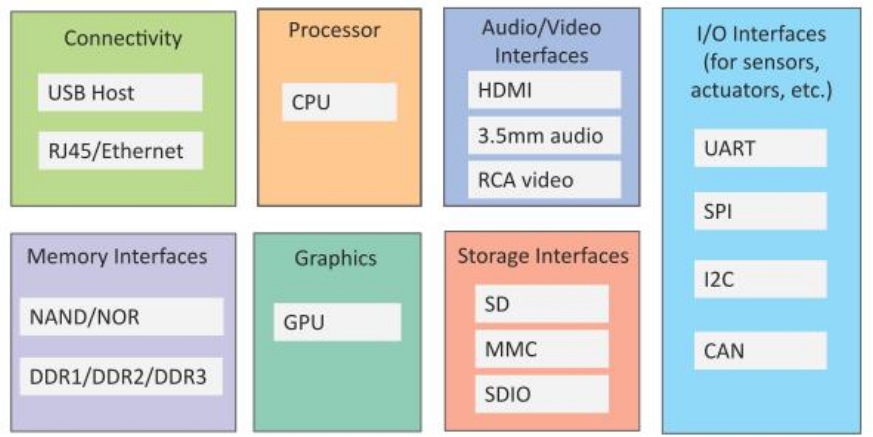
\includegraphics[width=12cm, height=7cm]{IoT/IOT1.jpg}
	\caption{Generic block diagram of an IoT Device}
\end{figure} 
}
\justify{
\\{\textbf{IoT Protocols of IoT}}\\
An IoT device may consist of several interfaces for connections to other devices, both wired and wireless\\
\\{\textbf{Link Layer}}
\begin{itemize}[noitemsep,nolistsep]
\item 802.3 – Ethernet
\item 802.11 – WiFi
\item 802.16 – WiMax
\item 802.15.4 – LR-WPAN
\item 2G/3G/4G
\end{itemize}}
\justify{
\\{\textbf{Network/Internet Layer}}
\begin{itemize}[noitemsep,nolistsep]
    \item IPv4
    \item IPv6
    \item 6LoWPAN
\end{itemize}}
\justify{
\\{\textbf{Transport Layer}}
\begin{itemize}[noitemsep,nolistsep]
    \item TCP   
    \item UDP
\end{itemize}}
\justify{
\\{\textbf{Application Layer}}
\begin{itemize}[noitemsep,nolistsep]
    \item HTTP
    \item CoAP
    \item WebSocket
    \item MQTT
    \item XMPP
    \item DDS
    \item AMQP 
\end{itemize}
\\
}
\begin{figure}[h!]
    \centering
	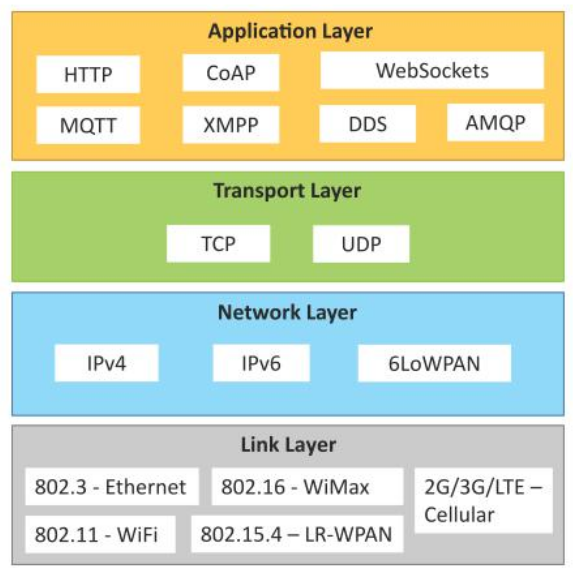
\includegraphics[width=12cm, height=10cm]{IoT/IOT2.jpg}
	\caption{Protocols of IoT}
\end{figure} 

\justify{
\\{\textbf{Logical Design of IoT}}
\begin{itemize}[noitemsep,nolistsep]
\item Logical design of an IoT system refers to an abstract representation of the entities and processes with out going into the low-level specifics of the implementation.
\end{itemize}
\vspace{5mm}
\\{\textbf{Functional Blocks of IoT}}

\begin{itemize}[noitemsep,nolistsep]
\item An IoT system comprises of a number of functional blocks that provide the system the capabilities for identification, sensing, actuation, communication, and management\end{itemize}}
\begin{figure}[h!]
    \centering
	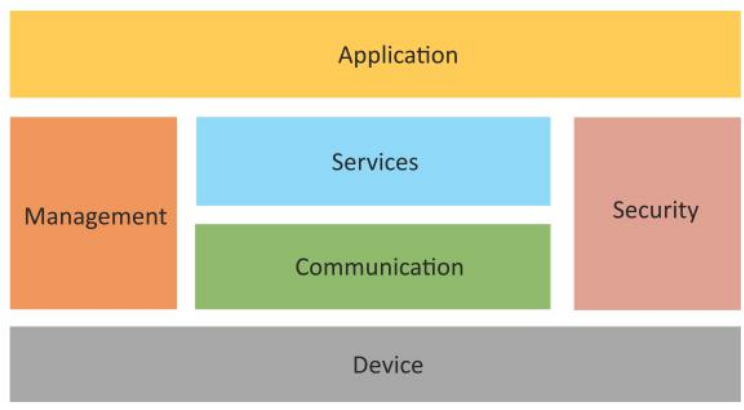
\includegraphics[width=12cm, height=8cm]{IoT/IOT3.jpg}
	\caption{Functional Blocks of IoT}
\end{figure} 
\vspace{5mm}
\justify{
\\{\textbf{Communication Blocks of IoT}}\\
\\{\textbf{Request-Response communication model}}\\
\begin{itemize}[noitemsep,nolistsep]
\item Request-Response is a communication model in which the client sends requests to the server and the server responds to the requests.
\item When the server receives a request, it decides how to respond, fetches the data, retrieves resource representations, prepares the response, and then sends the response to the client.
\end{itemize}}
\justify{
\\{\textbf{Publish-Subscribe Communication Model}}
\newline
Publish-Subscribe is a communication model that involves publishers, brokers and consumers. \\
\begin{itemize}[noitemsep,nolistsep]
\item Publishers are the source of data. Publishers send the data to the topics which are managed by the broker. Publishers are not aware of the consumers.
\item Consumers subscribe to the topics which are managed by the broker.
\item When the broker receives data for a topic from the publisher, it sends the data to all the subscribed consumers.\\
\end{itemize}}
\justify{
\\{\textbf{Exclusive Pair communication model}\\
Exclusive Pair is a bidirectional, fully duplex communication model that uses a persistent connection between the client and server.
}}

\justify{
\\{\textbf{REST-based Communication APIs}}\\
Representational State Transfer (REST) is a set of architectural principles by which you can design web services and web APIs that focus on a system’s resources and how resource states are addressed and transferred.
}

\justify{
\\{\textbf{WebSocket-based Communication APIs}}\\
WebSocket APIs allow bi-directional, full duplex communication between clients and servers.
}

\justify{
\\{\textbf{Exclusive Pair communication model}}\\
Exclusive Pair is a bidirectional, fully duplex communication model that uses a persistent connection between the client and server.}

\justify{
\\{\textbf{Levels and Deployment Templates in IoT}}
\\
An IoT system comprises of the following components:
\begin{itemize}[noitemsep,nolistsep]
\item {\textbf{Device:}} An IoT device allows identification, remote sensing, actuating and remote monitoring capabilities.
\item {\textbf{Resource:}} Resources are software components on the IoT device for accessing, processing, and storing sensor information, or controlling actuators connected to the device. Resources also include the software components that enable network access for the device.
\item {\textbf{Controller Service:}} Controller service is a native service that runs on the device and interacts with the web services. Controller service sends data from the device to the web service and receives commands from the application (via web services) for controlling the device.
\item {\textbf{Database:}} Database can be either local or in the cloud and stores the data generated by the IoT device.
\item {\textbf{Web Service:}} Web services serve as a link between the IoT device, application, database and analysis components. Web service can be either implemented using HTTP and REST principles (REST service) or using WebSocket protocol (WebSocket service). 
\item {\textbf{Analysis Component:}} The Analysis Component is responsible for analyzing the IoT data and generate results in a form which are easy for the user to understand.
\item {\textbf{Application:}} IoT applications provide an interface that the users can use to control and monitor various aspects of the IoT system. Applications also allow users to view the system status and view the processed data
\end{itemize}}

\justify{
\\{\textbf{IoT Level-1}}\\
\begin{itemize}[noitemsep,nolistsep]
\item A level-1 IoT system has a single node/device that performs sensing and/or
actuation, stores data, performs analysis and hosts the application
\item Level-1 IoT systems are suitable for modeling low- cost and low-complexity
solutions where the data involved is not big and the analysis requirements are 
not computationally intensive.
\end{itemize}
}
\justify{
\\{\textbf{IoT Level-2}}\\
\begin{itemize}[noitemsep,nolistsep] 
\item A level-2 IoT system has a single node that performs sensing and/or actuation and local analysis.
\item Data is stored in the cloud and application is usually cloud-based.
\item Level-2 IoT systems are suitable for solutions where the data involved is big,
however, the primary analysis requirement is not computationally intensive and can be done locally itself.
\end{itemize}
}
\justify{
\\{\textbf{IoT Level-3}}\\
\begin{itemize}[noitemsep,nolistsep] 
\item A level-3 IoT system has a single node. Data is stored and analyzed in the cloud and application is cloud- based.
\item Level-3 IoT systems are suitable for solutions where the data involved is big and the analysis requirements are computationally intensive. 
\end{itemize}
}
\justify{
\\{\textbf{IoT Level-4}}\\
\begin{itemize}[noitemsep,nolistsep] 
\item A level-4 IoT system has multiple nodes that perform local analysis. Data is stored in the cloud and application is cloud-based.
\item Level-4 contains local and cloud-based observer nodes which can subscribe to and receive information collected in the cloud from IoT devices.
\item Level-4 IoT systems are suitable for solutions where multiple nodes are required, the data involved is big and the analysis requirements are computationally intensive.
\end{itemize}}
\clearpage
\justify{
\\{\textbf{IoT Level-5}}\\
\begin{itemize}[noitemsep,nolistsep]
\item A level-5 IoT system has multiple end nodes and one coordinator node. 
\item The end nodes that perform sensing and/or actuation.
\item Coordinator node collects data from the end nodes and sends to the cloud.
\item Data is stored and analyzed in the cloud and application is cloud-based.
\item Level-5 IoT systems are suitable for solutions based on wireless sensor networks, in which the data involved is big and the analysis requirements are computationally intensive.
\end{itemize}}
\justify{
\\{\textbf{IoT Level-6}}\\
\begin{itemize}[noitemsep,nolistsep]
\item A level-6 IoT system has multiple independent end nodes that perform sensing and/or actuation and send data to the cloud.
\item Data is stored in the cloud and application is cloud-based.
\item The analytics component analyzes the data and stores the results in the cloud database.
\item The results are visualized with the cloud-based application.
\item The centralized controller is aware of the status of all the end nodes and ends control commands to the nodes.
\end{itemize}}

\begin{figure}[h!]
    \centering
	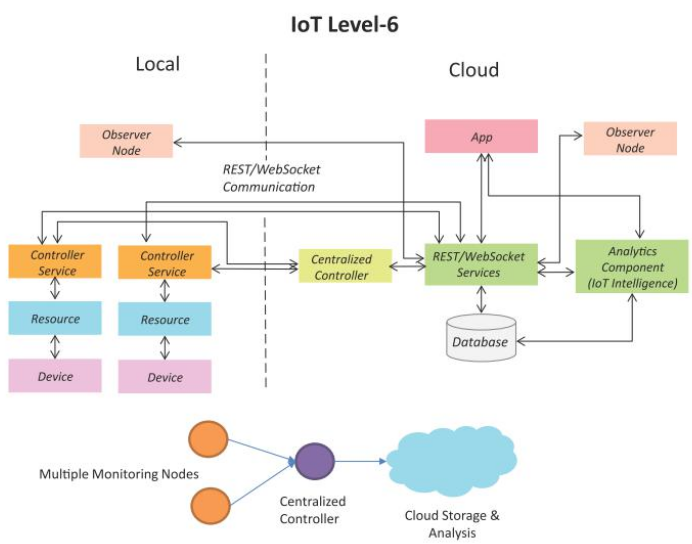
\includegraphics[width=15cm, height=12cm]{IoT/IOT6.jpg}
	\caption{IoT Level-6}
\end{figure} 

\centering{\textbf{Reference:} Bahga, A., & Madisetti, V. (2014). Internet of Things - A Hands-On Approach. Vijay Madisetti
Publishing/VPT. ISBN:978-0996025515.}
\clearpage
\begin{center}
{\large \textbf{Introduction to Arduino Uno}}
\end{center}
\justify{
\\{\textbf{Arduino Uno}} is a microcontroller board based on the ATmega328P (datasheet). It has 14 digital input/output pins (of which 6 can be used as PWM outputs), 6 analog inputs, a 16 MHz quartz crystal, a USB connection, a power jack, an ICSP header and a reset button. It contains everything needed to support the microcontroller.}
\\
\begin{figure}[h!]
    \centering
	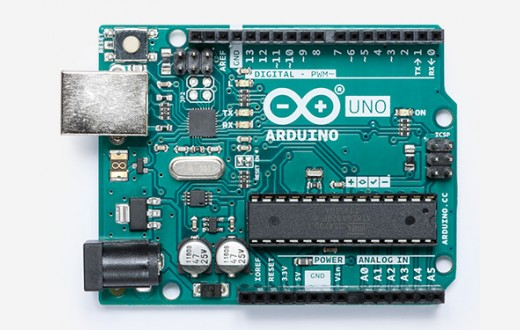
\includegraphics{Introduction/1.jpg}
	\caption{Arduino UNO Board}
	\caption*{\textbf{Source} - https://store.arduino.cc/usa/arduino-uno-rev3}
\end{figure}

\textbf{Detailed description of the Arduino UNO Board (Arduino Pinout Diagram)}\\

Arduino is open source hardware platform comes with Free and open source software IDE. Arduino is inexpensive, cross-platform, simple, has clear programming environment and extensible hardware and software platform.
\vspace{5mm}
\\
\textbf{Working with Arduino Uno} 
\begin{itemize}[noitemsep,nolistsep]
    \item Arduino Web Editor 
    \item Arduino IDEs
\end{itemize}
\vspace{5mm}
\textbf{Downloading the Arduino IDE}
\begin{itemize}[noitemsep,nolistsep]
	\item Choose the right distribution from the link -  https://www.arduino.cc/en/Main/Software
	\item To use Arduino IDE on Raspberry Pi3, download the arm distribution.
	\item On Ubuntu Installed PCs follow - https://www.arduino.cc/en/Guide/Linux
\end{itemize}
\vspace{5mm}
Before working on Arduino IDE and the Arduino uno, set necessary permissions for user preferred USB Ports. Make sure the Arduino is detected in the devices list through USB when connected to the USB port of Raspberry Pi/ Laptop/ Desktop Computers.
\begin{figure}[h!]
    \centering
	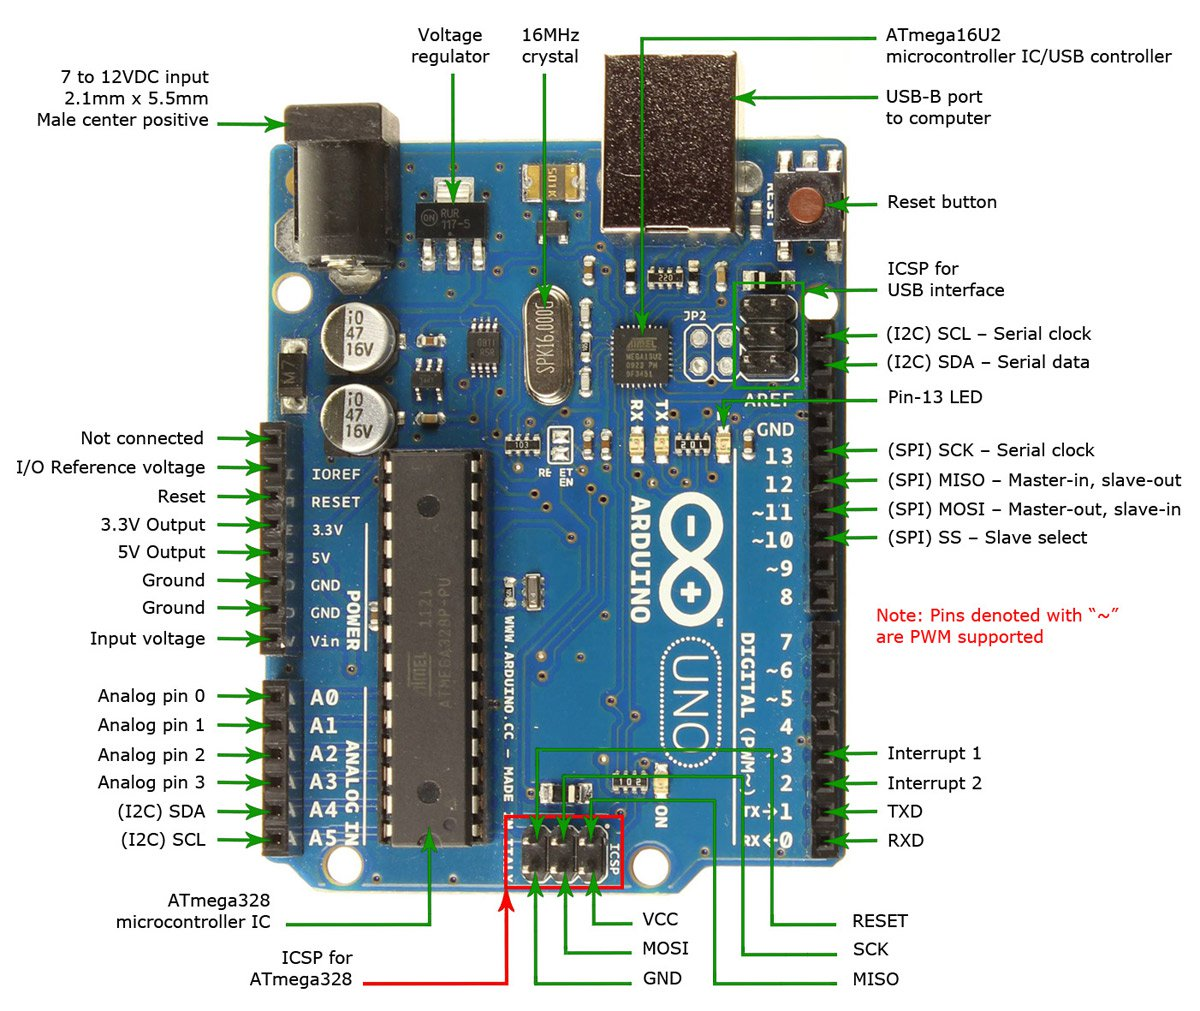
\includegraphics[width=12cm, height=11cm]{Introduction/2.jpg}
	\caption{Arduino Pinout Diagram}
	\caption*{\textbf{Source} - \url{https://www.jameco.com/}}
\end{figure}

\begin{table}[h!]
\begin{tabular}{|l|l|}
\hline
Microcontroller & ATMega328p \\ \hline
Operating Voltage & 5V \\ \hline
Input Voltage (recommended) & 7-12V \\ \hline
Input Voltage (limit) & 6-20V \\ \hline
Digital I/O Pins & 14 (of which 6 provide PWM output) \\ \hline
PWM Digital I/O Pins & 6 \\ \hline
Analog Input Pins & 6 \\ \hline
DC Current per I/O Pin & 20 mA \\ \hline
DC Current for 3.3V Pin & 50 mA \\ \hline
Flash Memory & 32 KB (ATmega328P) of which 0.5 KB used by bootloader \\ \hline
SRAM & 2 KB (ATmega328P) \\ \hline
EEPROM & 1 KB (ATmega328P) \\ \hline
Clock Speed & 16 MHz \\ \hline
LED\_BUILTIN & 13 \\ \hline
Length and width & 68.6 mm and 53.4 mm \\ \hline
Weight & 25 g \\ \hline
\end{tabular}
\end{table}
\\
\textbf{Arduino IDE with Arduino UNO Board}\\
Open the Arduino IDE and the Terminal 
\begin{figure}[h!]
    \centering
	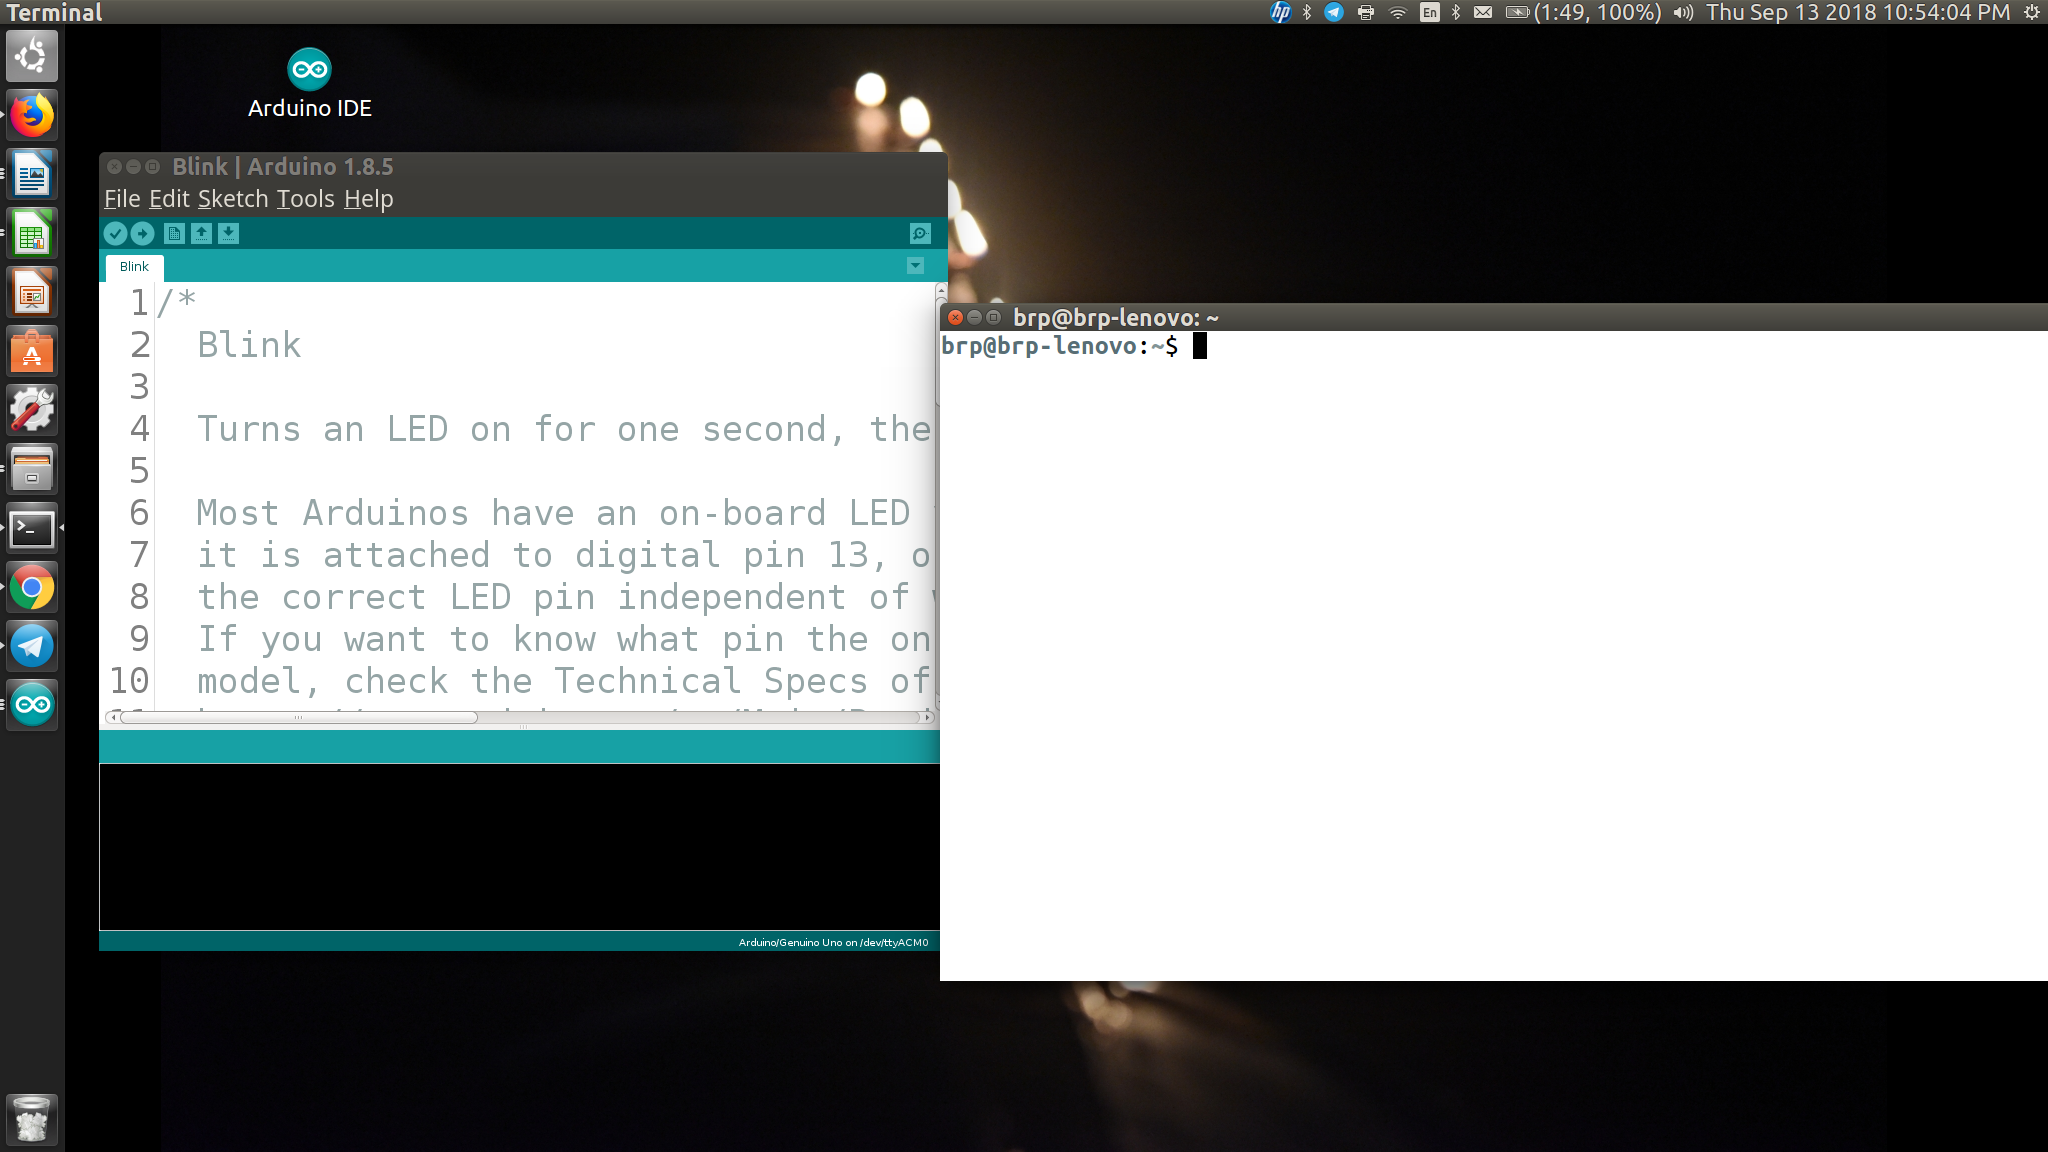
\includegraphics[width=15cm, height=10cm]{Introduction/3.png}
\end{figure}
\\
If previously worked on IDE and a UNO was used that can be seen being listed on the IDE (bottom right corner) 
\begin{figure}[h!]
    \centering
	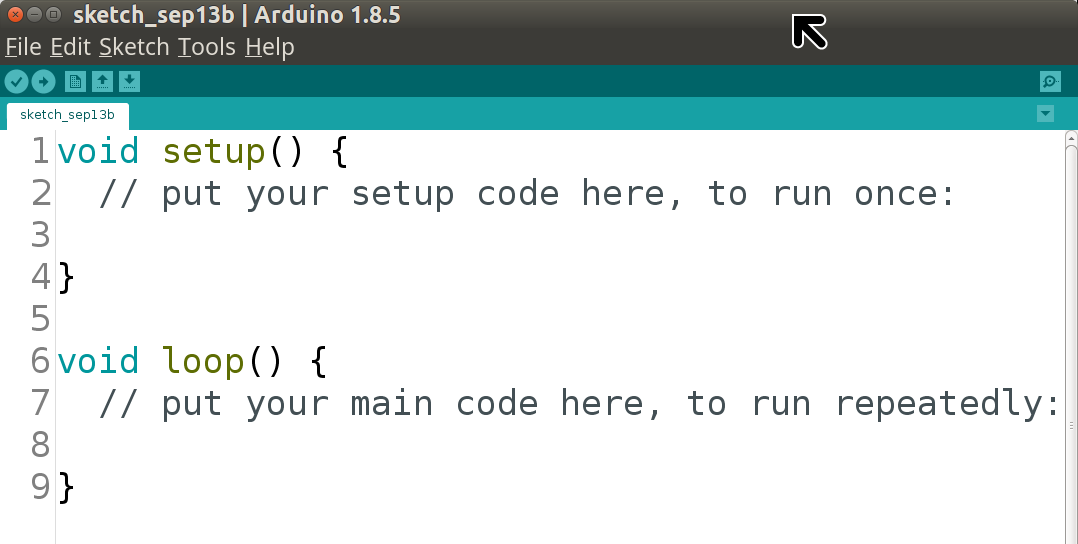
\includegraphics[width=15cm, height=8cm]{Introduction/4.png}
\end{figure}
\clearpage
\textbf{Procedure to check the Arduino Device Connection from the Terminal and through IDE}
\begin{figure}[h!]
    \centering
	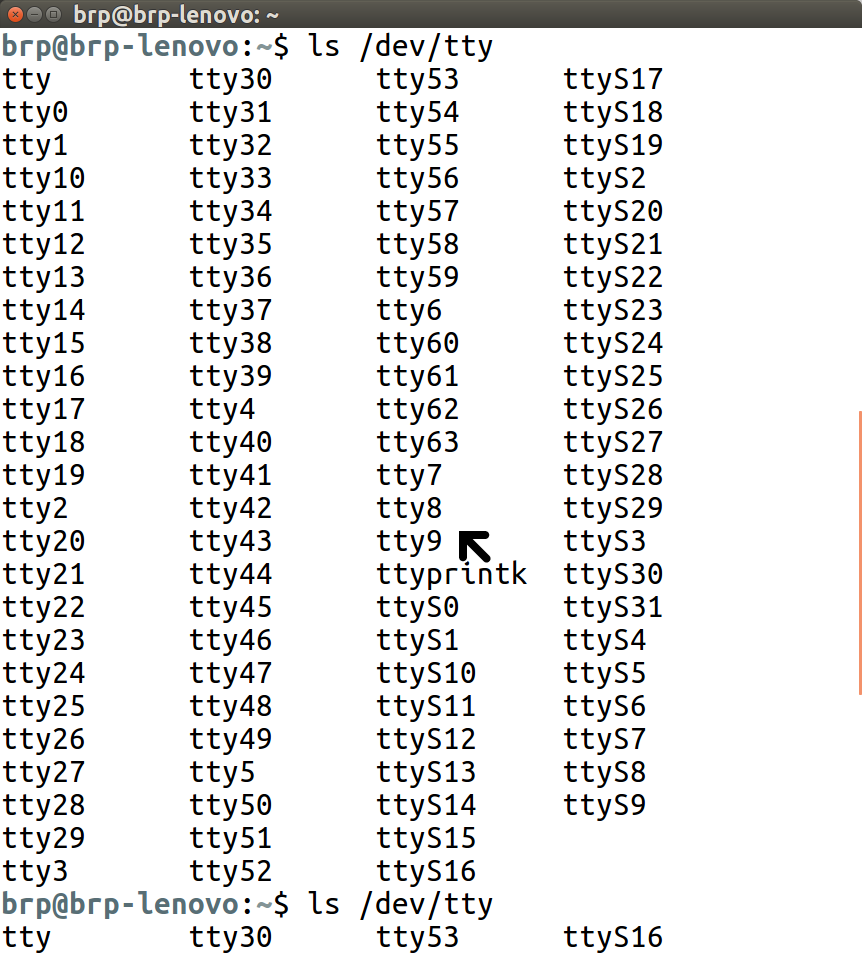
\includegraphics[width=15cm, height=13cm]{Introduction/5.png}
\end{figure}
\begin{figure}[h!]
    \centering
	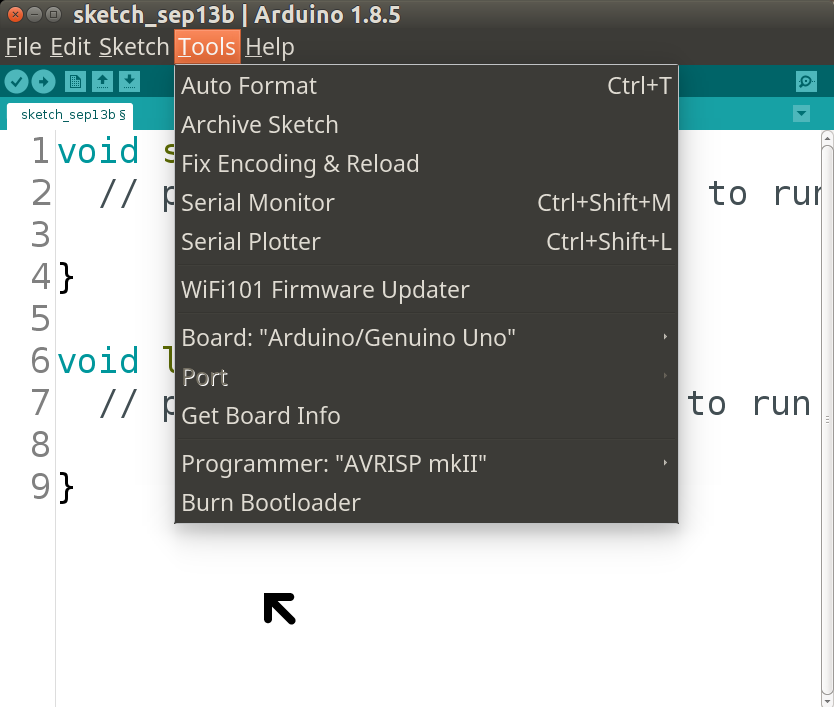
\includegraphics[width=15cm, height=9cm]{Introduction/6.png}
\end{figure}
\clearpage
\textbf{Now connect the Arduino through USB port and confirm the port \& the Board information are correlated in the IDE from the Tools Menu}\\
\begin{figure}[h!]
    \centering
	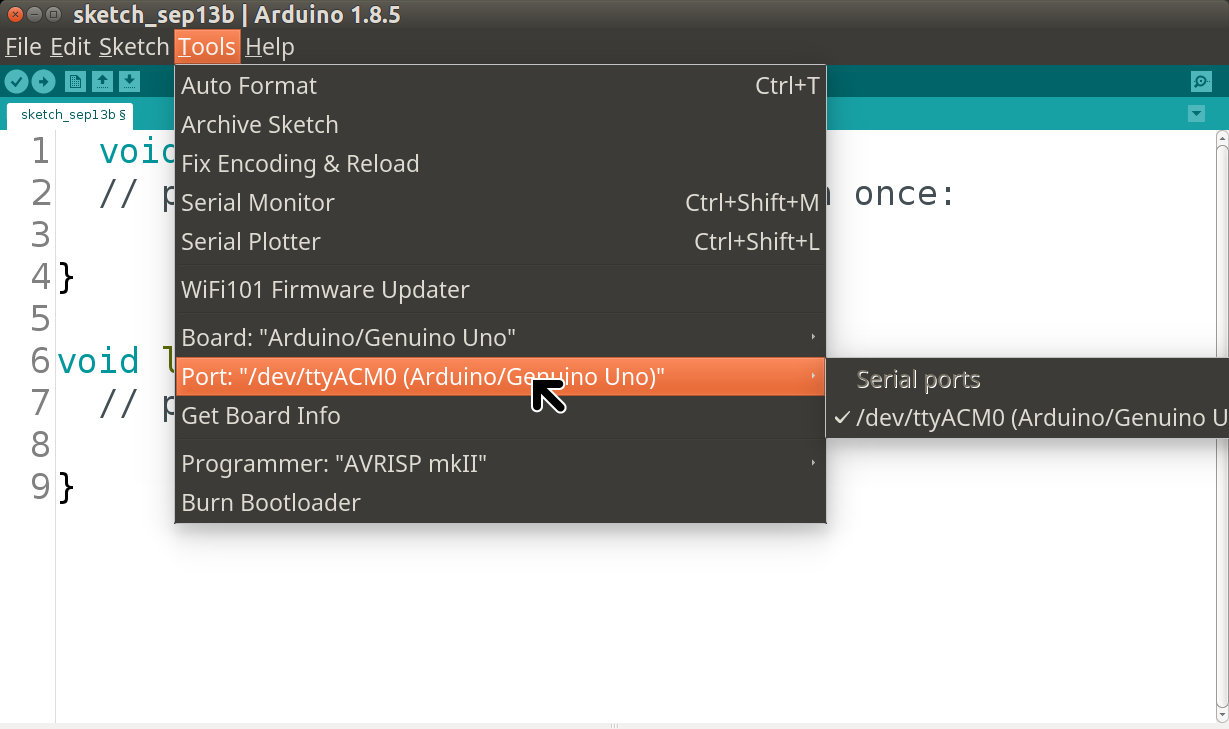
\includegraphics[width=15cm, height=9cm]{Introduction/7.png}
\end{figure}
\begin{figure}[h!]
    \centering
	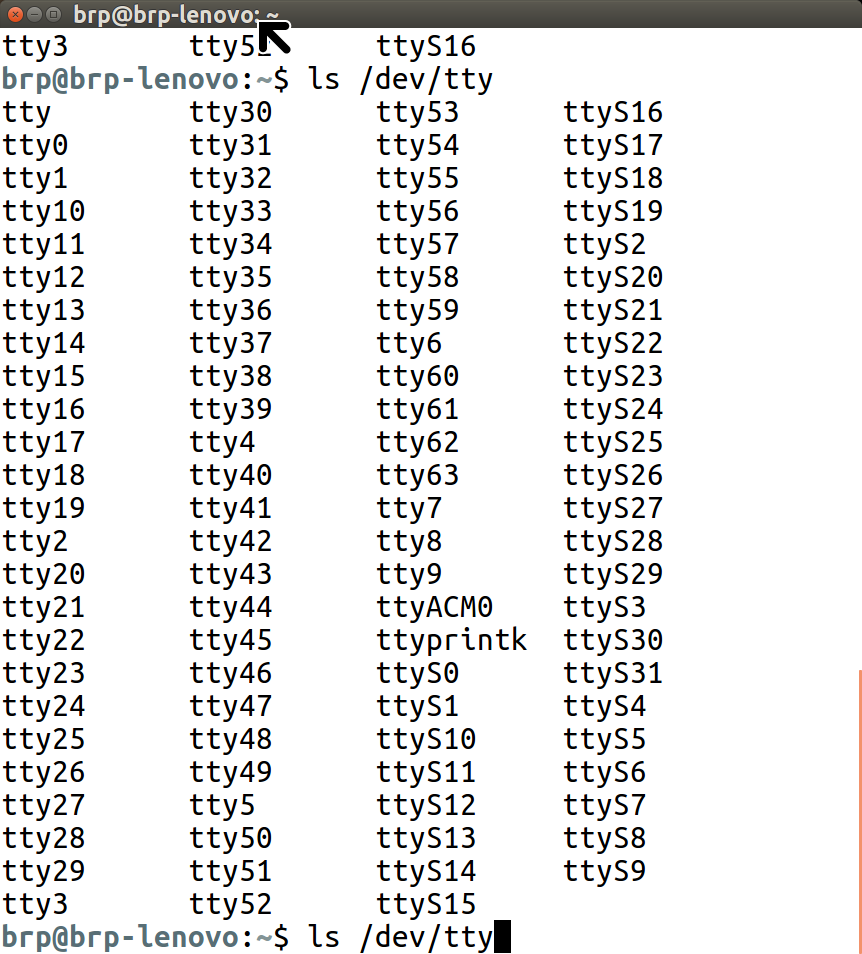
\includegraphics[width=15cm, height=13cm]{Introduction/8.png}
\end{figure}
\vspace{2mm}

\textbf{Working with default Example Sketches and Upload Procedure}\\
\begin{figure}[h!]
    \centering
	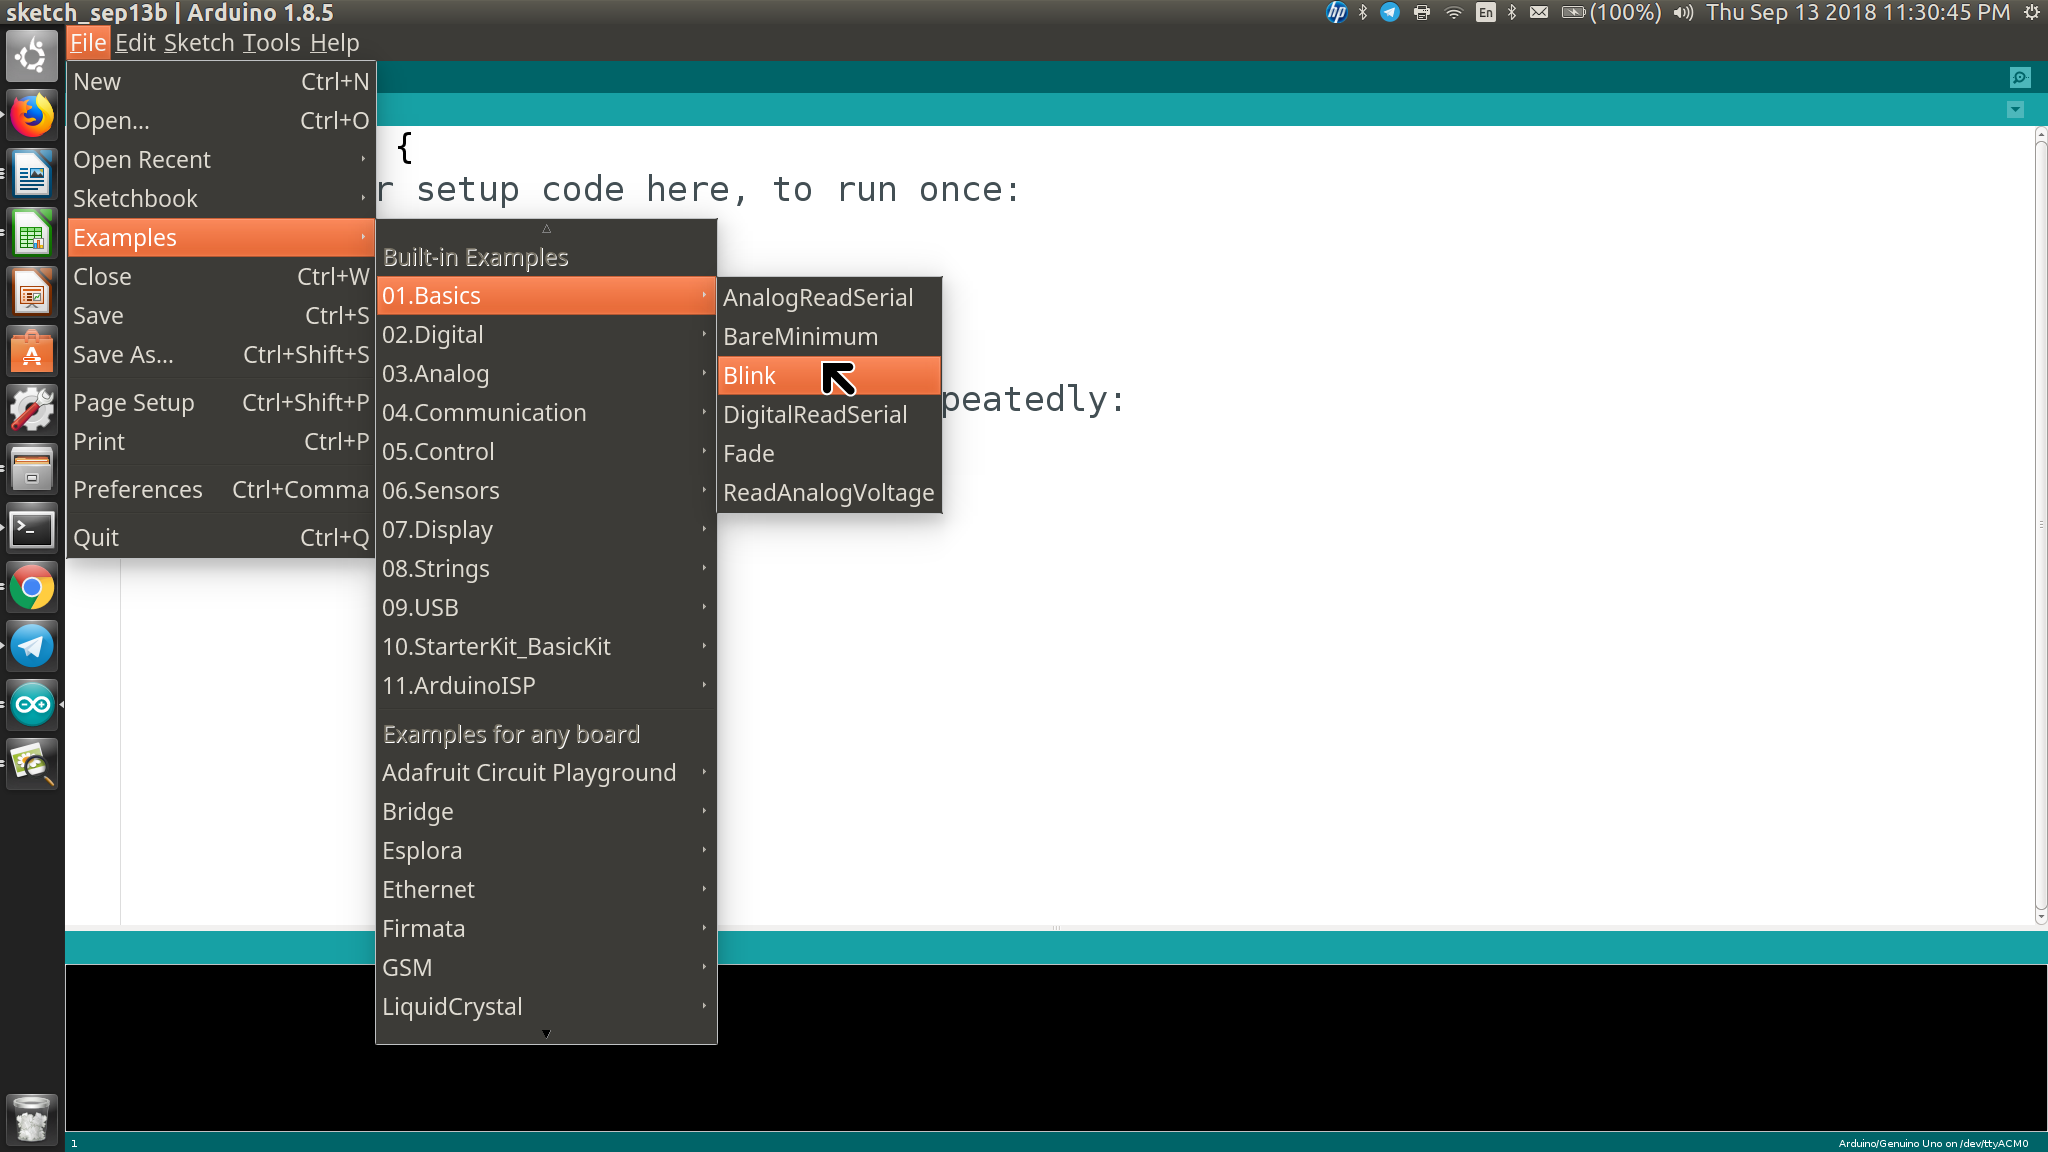
\includegraphics[width=15cm, height=10cm]{Introduction/9.png}
\end{figure}
\vspace{2mm}
\\
\textbf{Verify + Compile + Upload Sketch on to Arduino UNO}
\begin{figure}[h!]
    \centering
	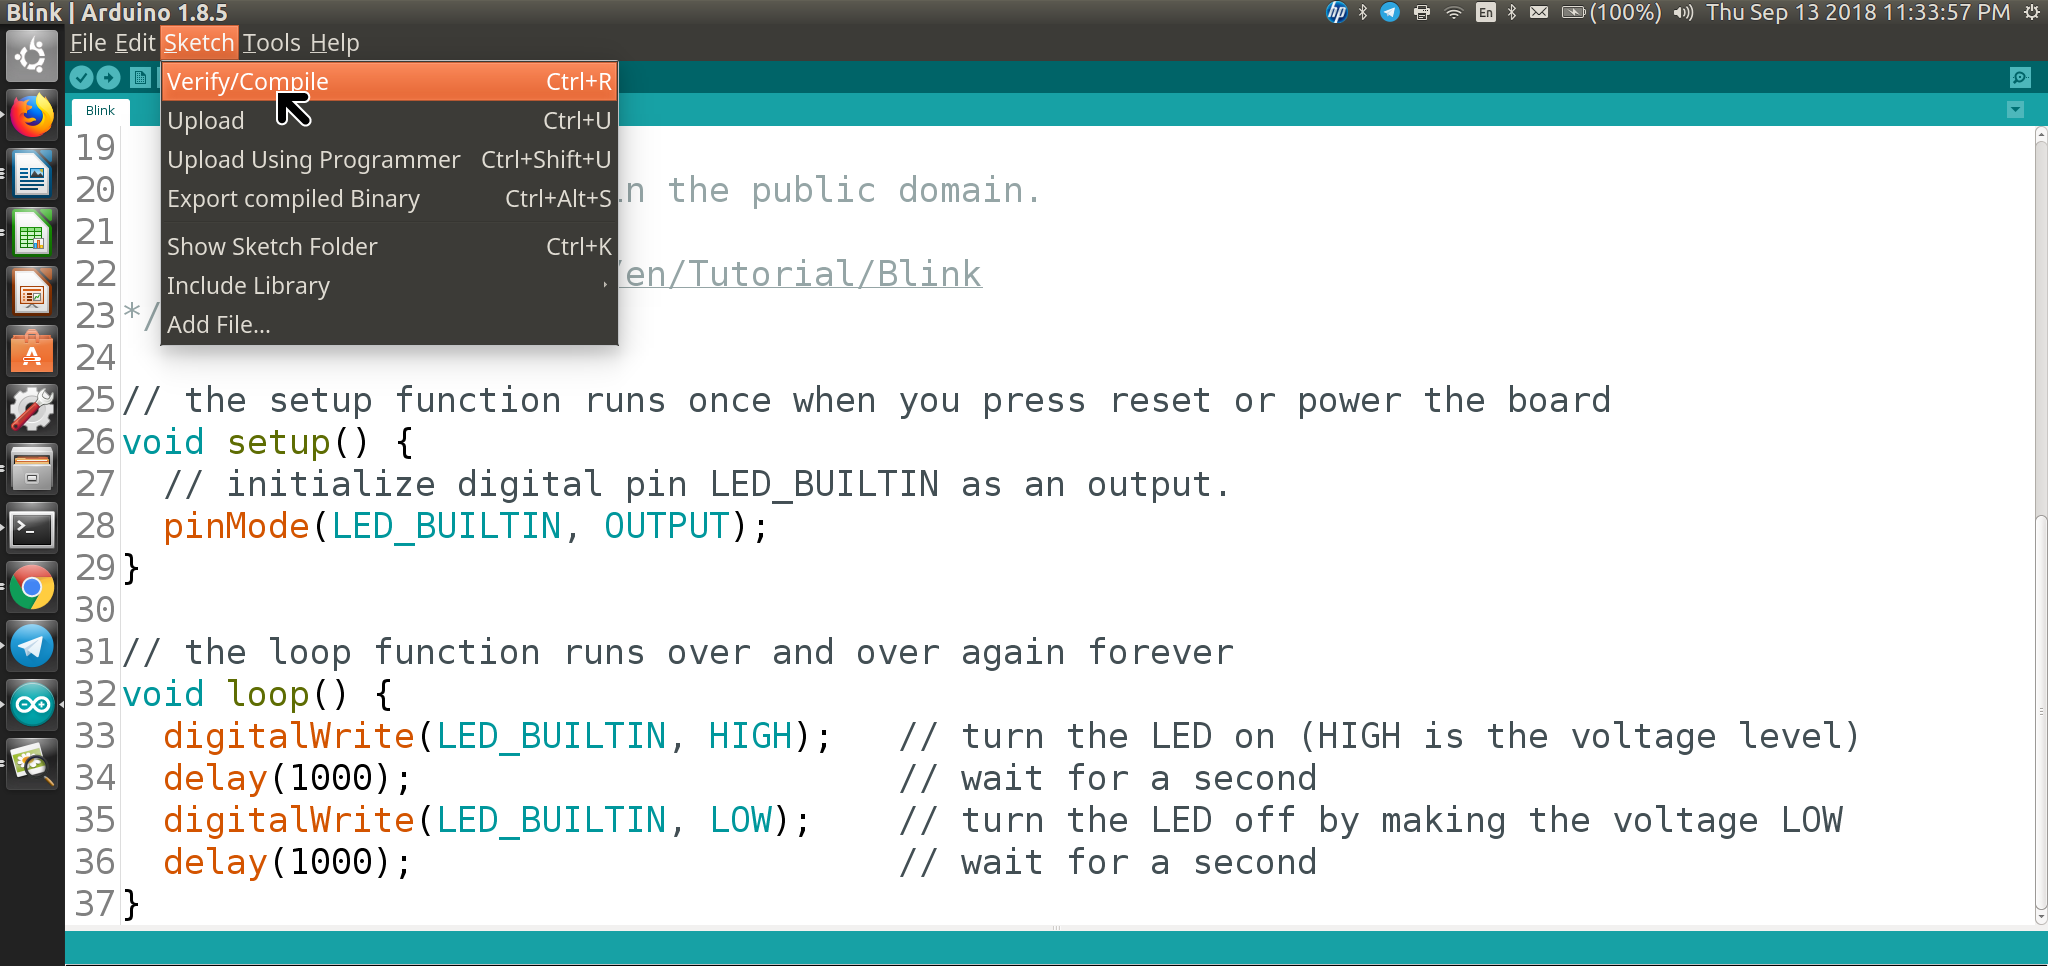
\includegraphics[width=15cm, height=10cm]{Introduction/10.png}
\end{figure}
\clearpage
\begin{center}
\large \textbf{Introduction to Raspberry Pi}
\end{center}
\justify{
\\{\textbf{Raspberry Pi}} is a low cost, credit-card sized computer that plugs into a computer monitor or TV, and uses a standard keyboard and mouse. It is a capable little device that enables people of all ages to explore computing, and to learn how to program in languages like Scratch and Python. It’s capable of doing everything you’d expect a desktop computer to do, from browsing the internet and playing high-definition video, to making spreadsheets, word-processing, and playing games.}
\begin{figure}[h!]
    \centering
	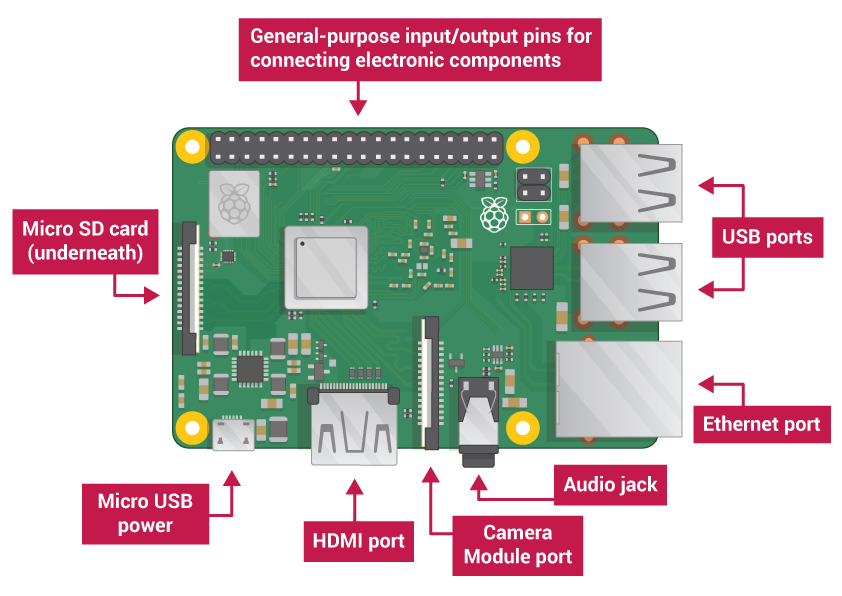
\includegraphics[width=12cm, height=7cm]{Introduction/11.png}
	\caption{Raspberry Pi3 B Board Specification}
	\caption*{\textbf{Source:}https://projects.raspberrypi.org/en/projects/raspberry-pi-getting-started/3}
\end{figure}
\begin{figure}[h!]
    \centering
	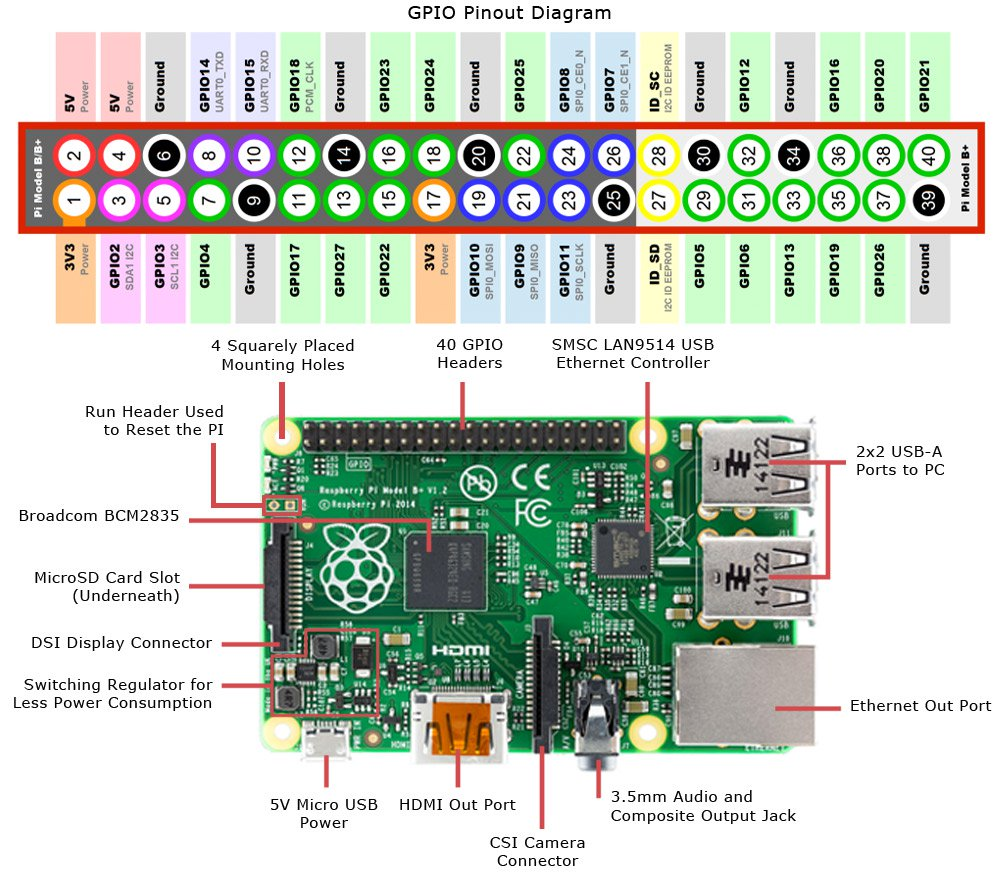
\includegraphics[width=12cm, height=10cm]{Introduction/13.jpg}
	\caption{GPIO Pinout Diagram of RaspberryPi3 B+}
\end{figure}
\begin{figure}[p]
\centering
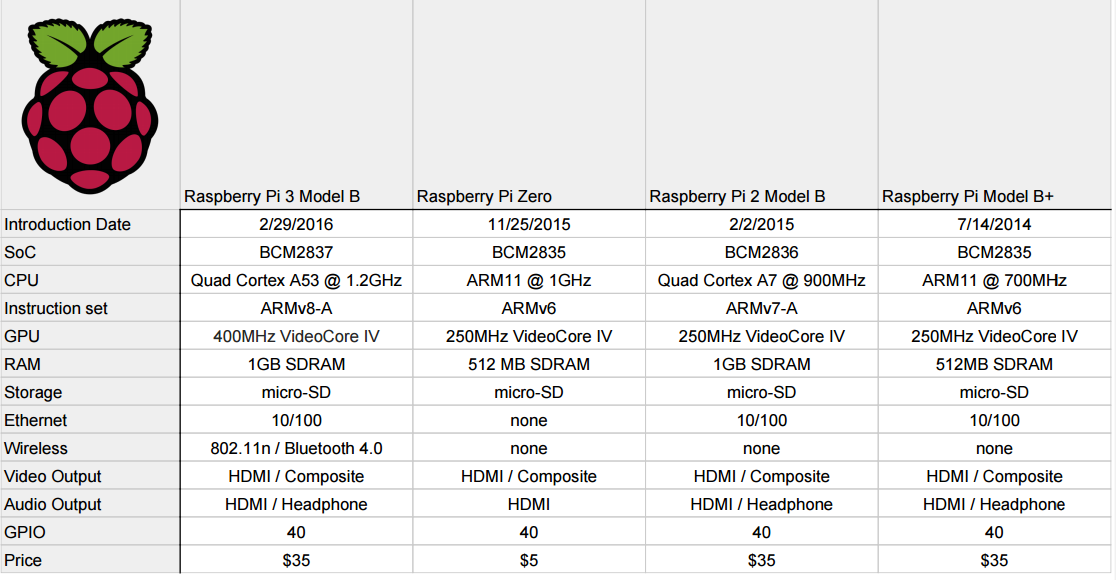
\includegraphics[width=1.3\textwidth, angle=90 ]{Introduction/12.png}
\caption{Raspberry Pi 3 and other board’s technical specification}
\caption*{\textbf{Source:} https://hackaday.com/2016/02/28/introducing-the-raspberry-pi-3/}
\end{figure}
\begin{figure}[h!]
    \centering
	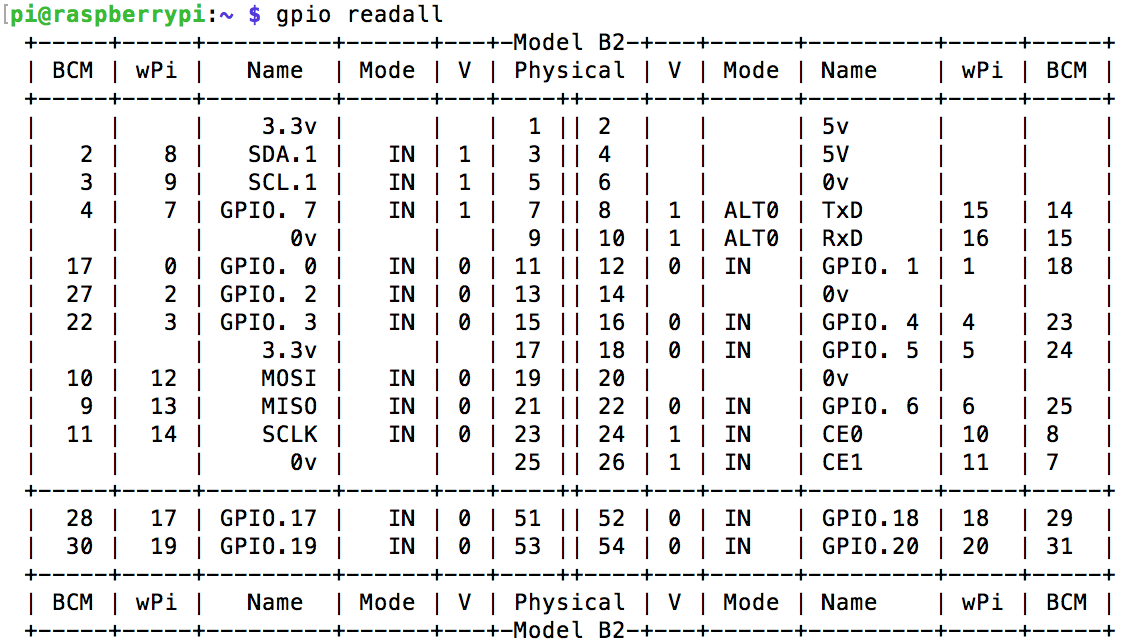
\includegraphics[width=15cm, height=12cm]{Introduction/14.png}
	\caption{GPIO Pinout Specifications of Raspberry Pi3 B+}
\end{figure}
\begin{figure}[h!]
    \centering
	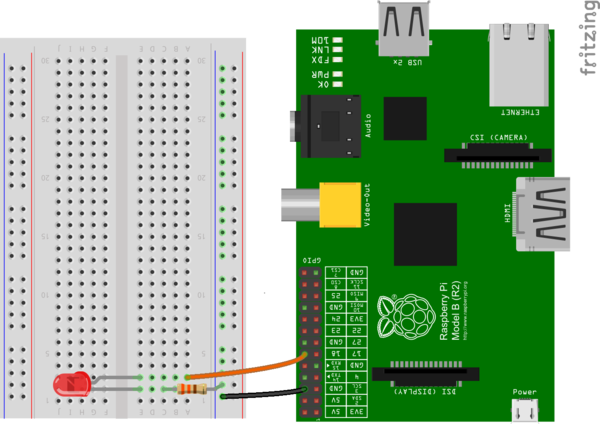
\includegraphics[width=12cm, height=8cm]{Introduction/15.png}
	\caption{Sample Program on Raspberry Pi2}
\end{figure}
\begin{lstlisting}
$nano LED.py

import RPi.GPIO as GPIO
import time
GPIO.setmode(GPIO.BCM)
GPIO.setwarnings(False)
GPIO.setup(18,GPIO.OUT)
print "LED on"
GPIO.output(18,GPIO.HIGH)
time.sleep(1)
print "LED off"
GPIO.output(18,GPIO.LOW)

$sudo python LED.py

\end{lstlisting}

\begin{center}
\large \textbf{Introduction to NodeMCU}
\end{center}
\justify{
\\{\textbf{NodeMCU}} is an open source firmware and development kit that helps you to prototype your IoT product with Arduino IDE or in few Lau script lines.
It includes firmware which runs on the ESP8266 Wi-Fi SoC. And hardware which is based on the ESP-12 module.
}
\begin{figure}[h!]
    \centering
	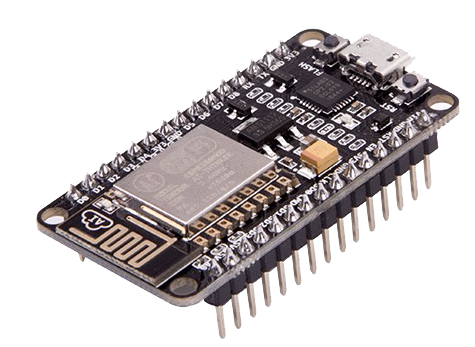
\includegraphics[width=15cm, height=8cm]{Introduction/16.png}
	\caption{Representation of NodeMCU}
\end{figure}

\textbf{NodeMCU Specifications} 
\begin{itemize}[noitemsep,nolistsep]
    \item Voltage:3.3V
    \item Current consumption: 10uA~170mA.
    \item Flash memory attachable: 16MB max (512K normal).
    \item Integrated TCP/IP protocol stack.
    \item Processor: Tensilica L106 32-bit.
    \item Processor speed: 80~160MHz.
    \item 4MB Flash Memory (default)
    \item GPIOs: 13 (multiplexed with other functions).
    \item Analog to Digital: 1 input with 1024 step resolution.
    \item Maximum concurrent TCP connections: 5
\end{itemize}
\vspace{5mm}

\justify{\textbf{Instructions related to the Power supply:}
\\
The ESP8266 chip requires 3.3V power supply voltage. It should not be powered with 5 volts like other Arduino boards.}
\\
\begin{itemize}[noitemsep,nolistsep]
    \item NodeMCU ESP-12E dev board can be connected to 5V using micro USB connector or Vin pin available on board.
    \item The I/O pins of ESP8266 communicate or input/output max 3.3V only. i.e. the pins are NOT 5V tolerant inputs. 
\end{itemize}
\\
To interface with 5V I/O pins, use level conversion system. 
\begin{figure}[h!]
    \centering
	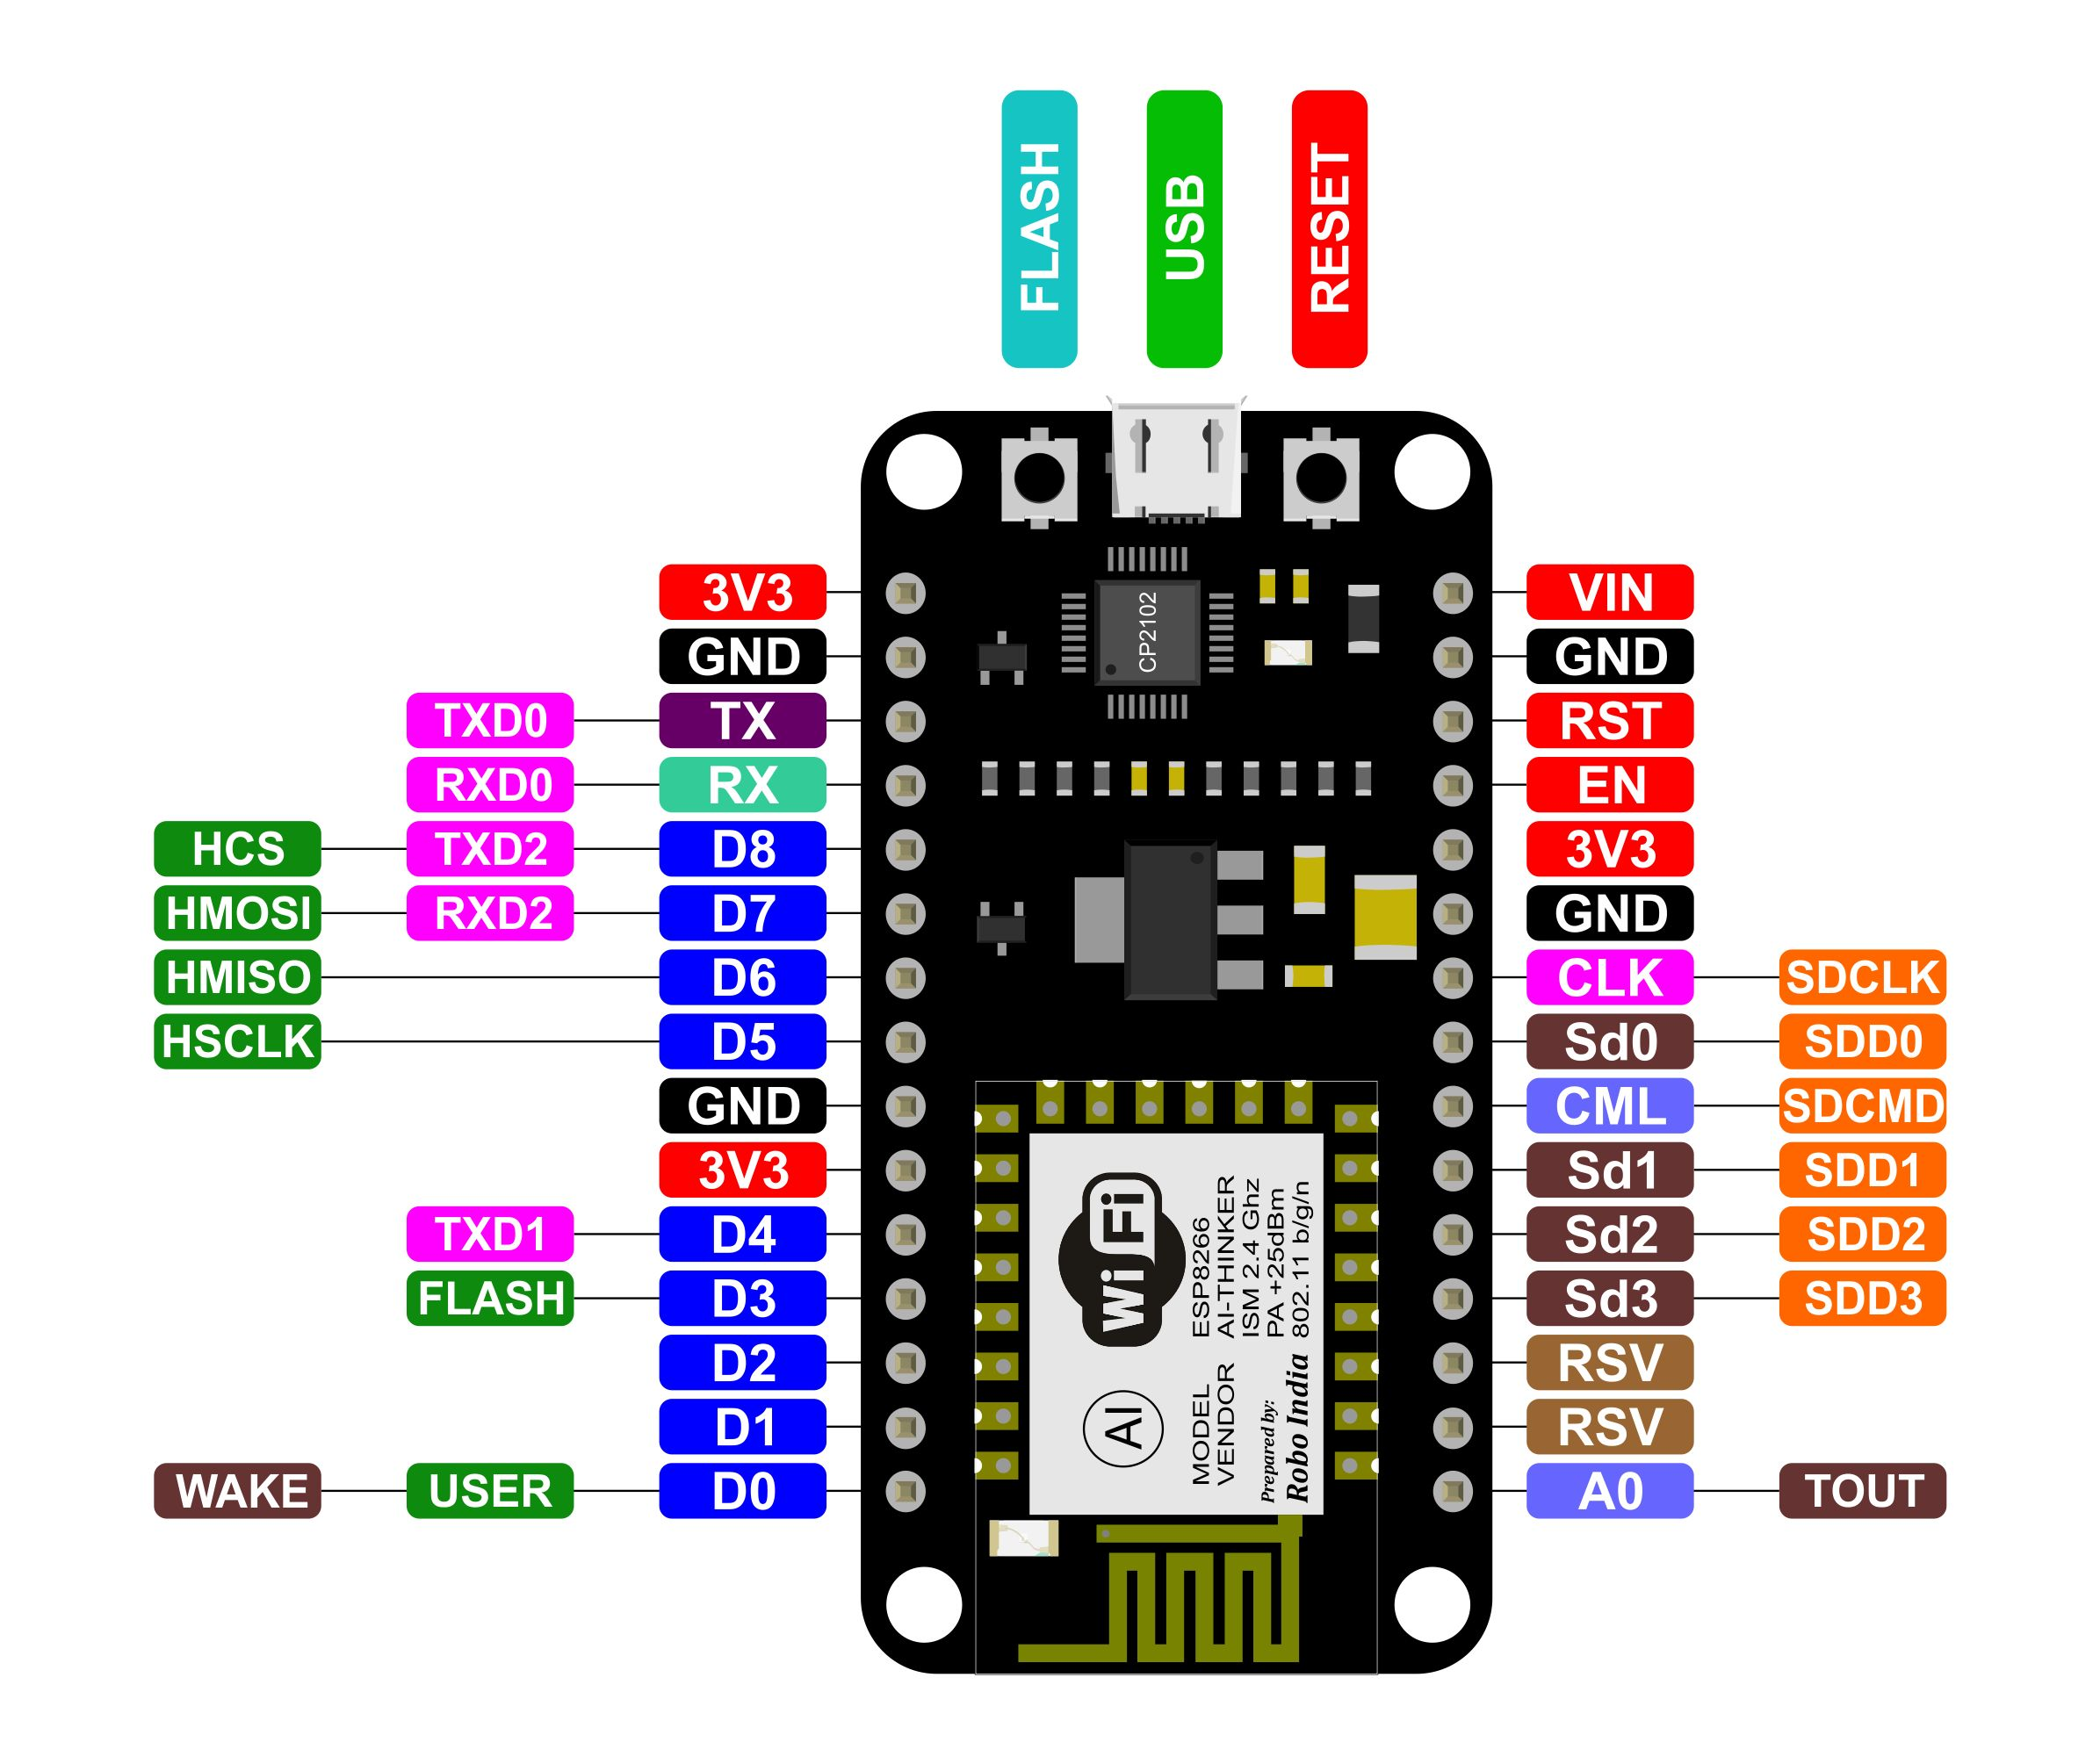
\includegraphics[width=15cm, height=10cm]{Introduction/17.jpg}
	\caption{Pinout Specifications of NodeMCU}
\end{figure}

\textbf{Installation of Micro Python Firmware}\\

Download the latest MicroPython firmware .bin file to load onto your ESP8266 device. Choose the files that are stable firmware from http://micropython.org/download#esp8266
\\
To configure and work with esp8266 using Micro Python -
Refer the following link \\
https://docs.micropython.org/en/latest/esp8266/esp8266/tutorial/index.html \\
\clearpage
\textbf{Example of working with NodeMCU and LED}
\\
Components Required:
\begin{itemize}
    \item NodeMCU
    \item LED
    \item Jumper wires
\end{itemize} 
\textbf{Source:} https://micropython-on-esp8266-workshop.readthedocs.io/en/latest/basics.html
\begin{figure}[h!]
    \centering
	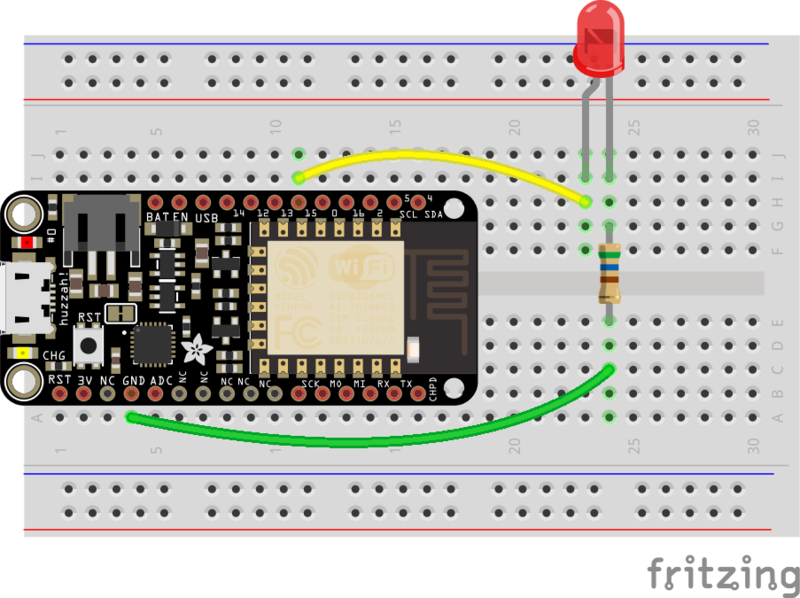
\includegraphics[width=11cm, height=8cm]{Introduction/18.png}
\end{figure}
\justify{Demonstrating the LED with NodeMCU using the digital pin D7 on board (GPIO-13) as a signal. The circuit for connecting LED to NodeMCU is as shown in the diagram above. LED has a slightly longer led to know it as a cathode and shorter leg as a anode. Anode of LED is connected to GND and Cathode is connected to the D7 on board (GPIO-13).}\\
\begin{figure}[h!]
    \centering
	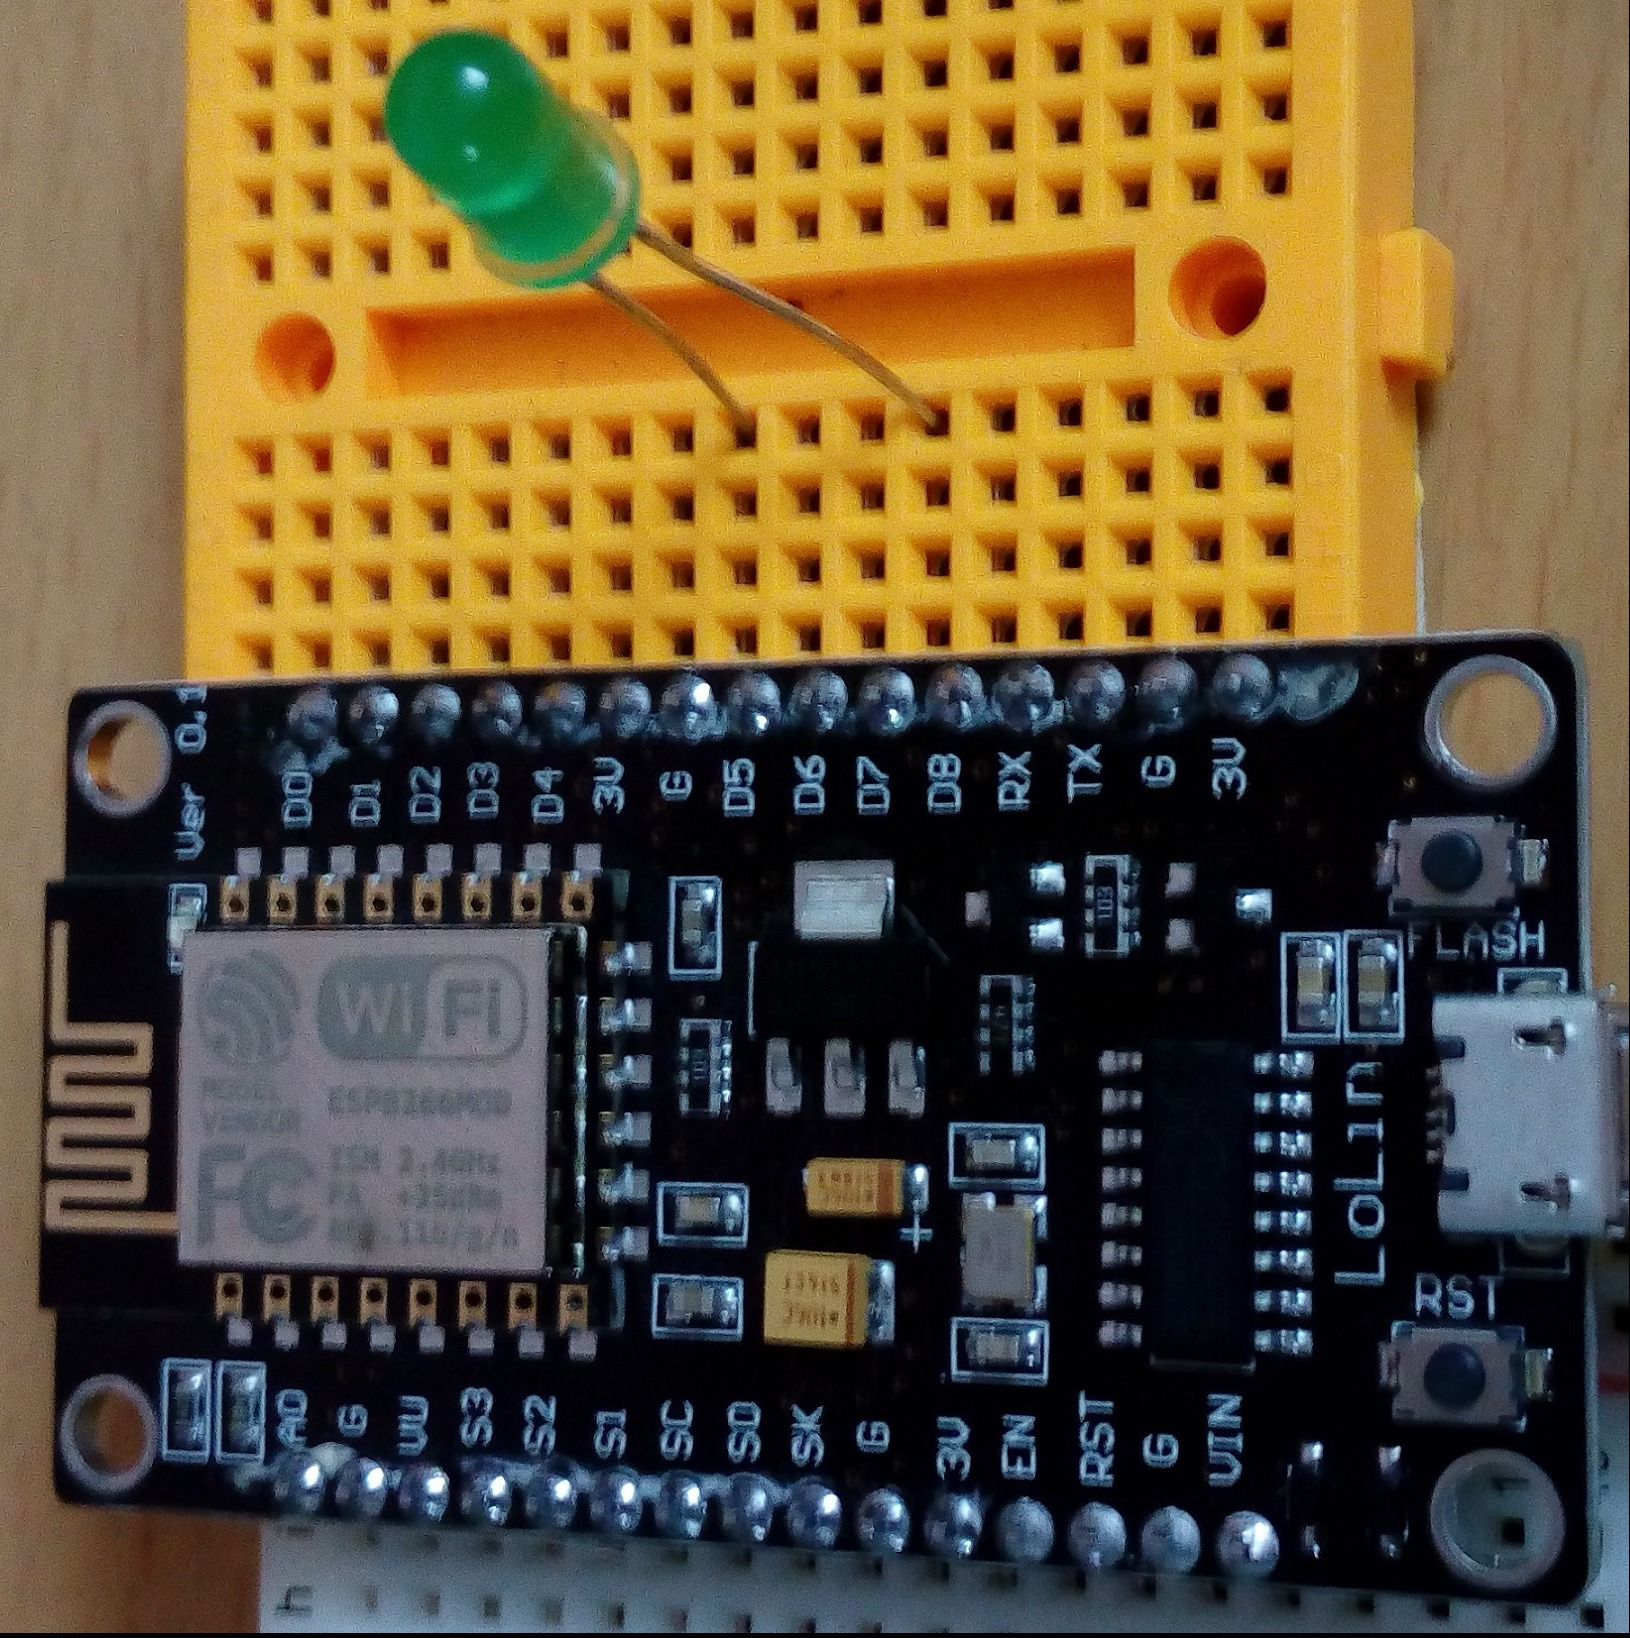
\includegraphics[width=10cm, height=9cm]{Introduction/19.jpg}
	\caption{Connection Screen Shot for LED}
\end{figure}

\textbf{Code for LED Connection}\\

\begin{lstlisting}
    >>> import machine, time
    >>> pin=machine.Pin(13,machine.Pin.OUT)
    >>> while(True):
    ...     if(pin.value()==0):
    ...         pin.on()
    ...         time.sleep(1)
    ...     else:
    ...         pin.off()
    ...         time.sleep(1)
\end{lstlisting}
\begin{figure}[h!]
\centerline{%
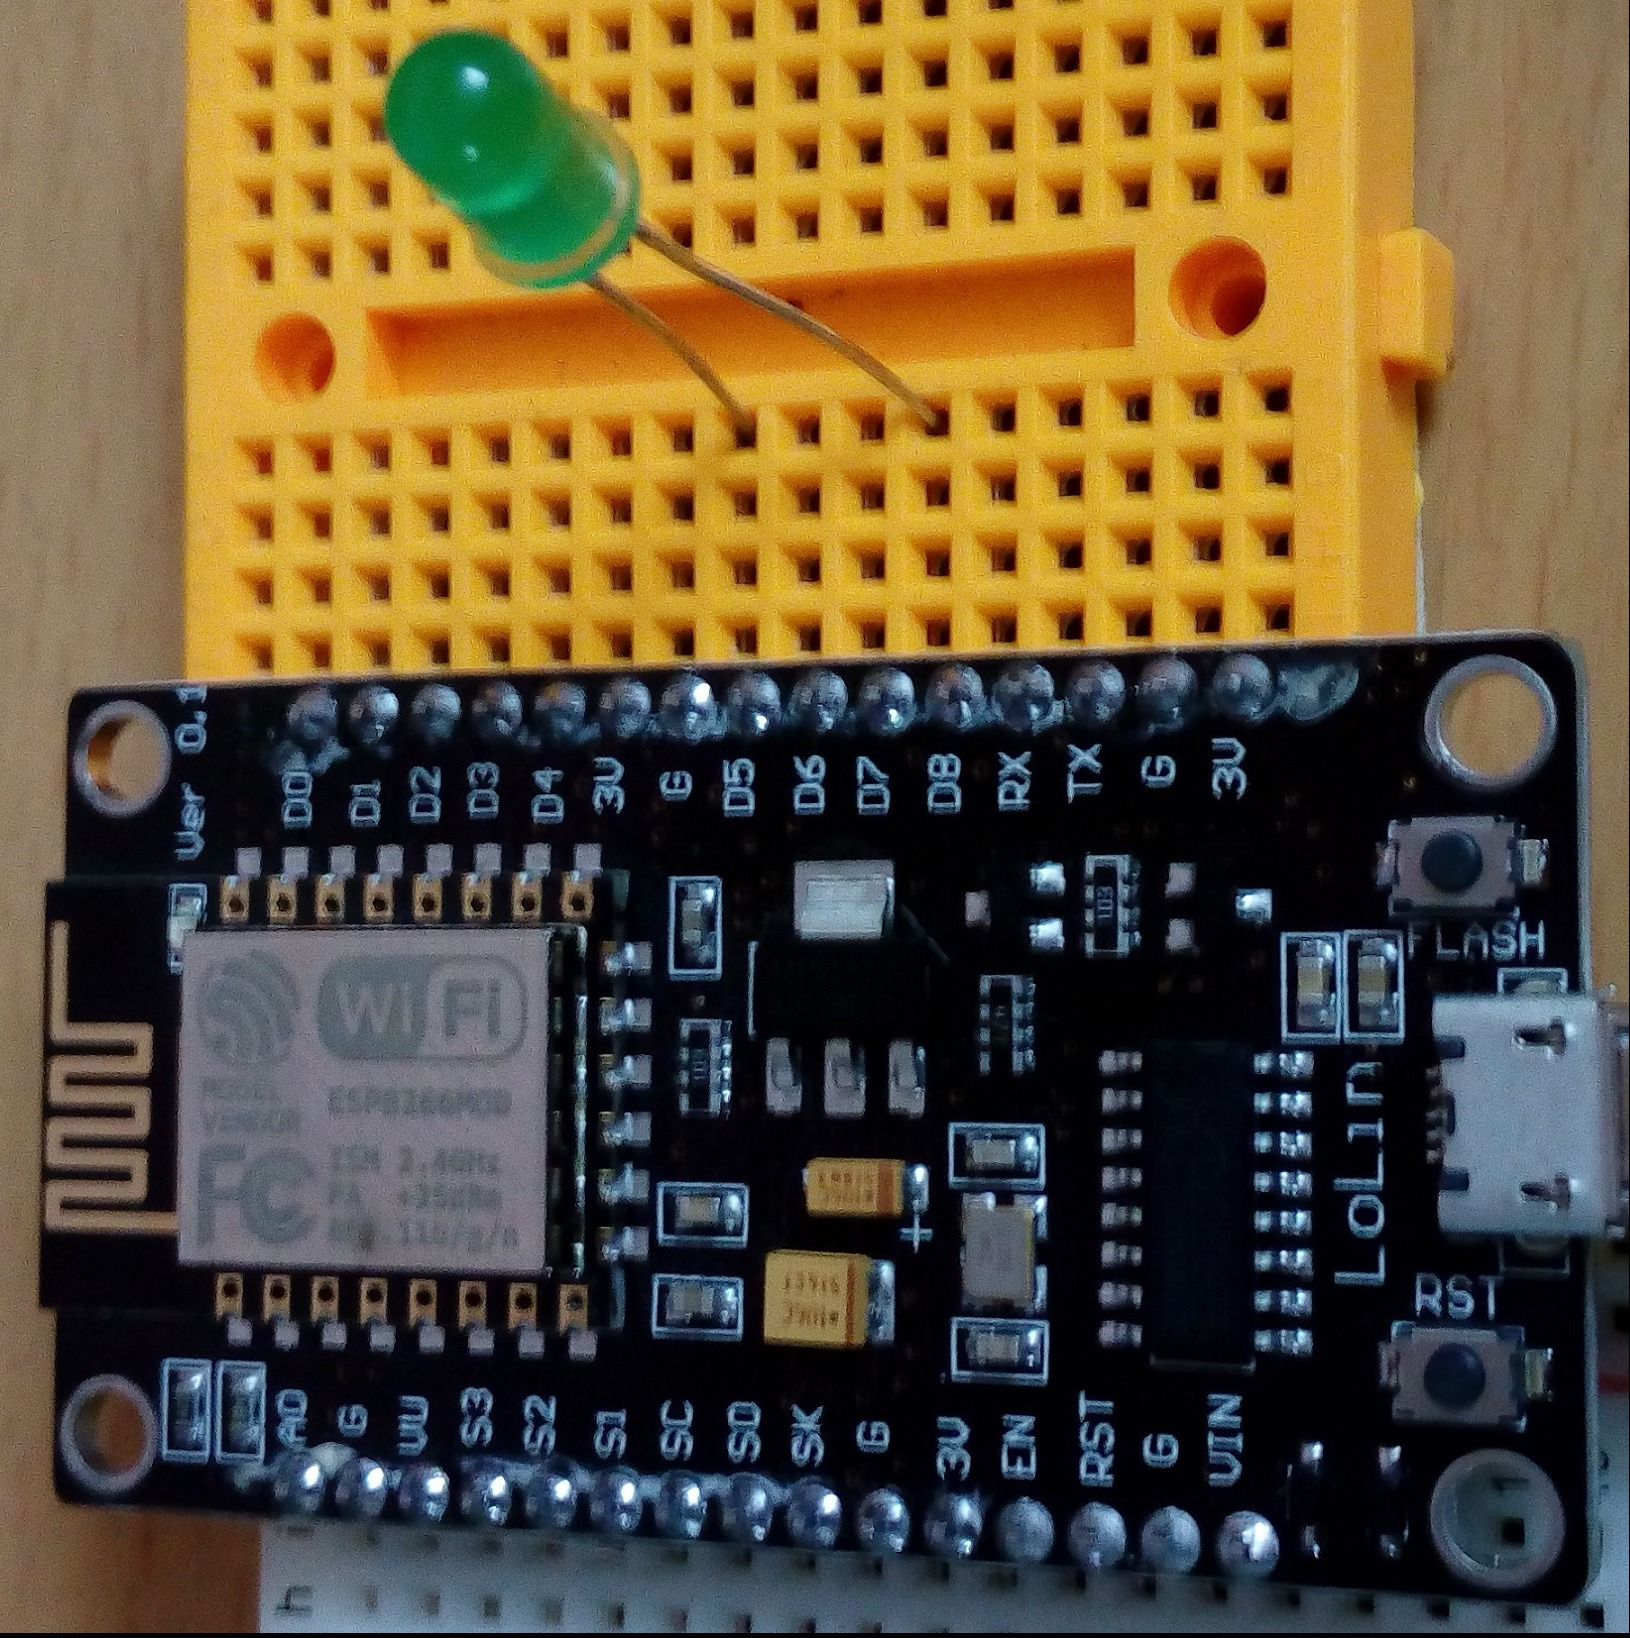
\includegraphics[width=8cm,height=8cm]{Introduction/20a.jpg}
\vspace{0.5mm}
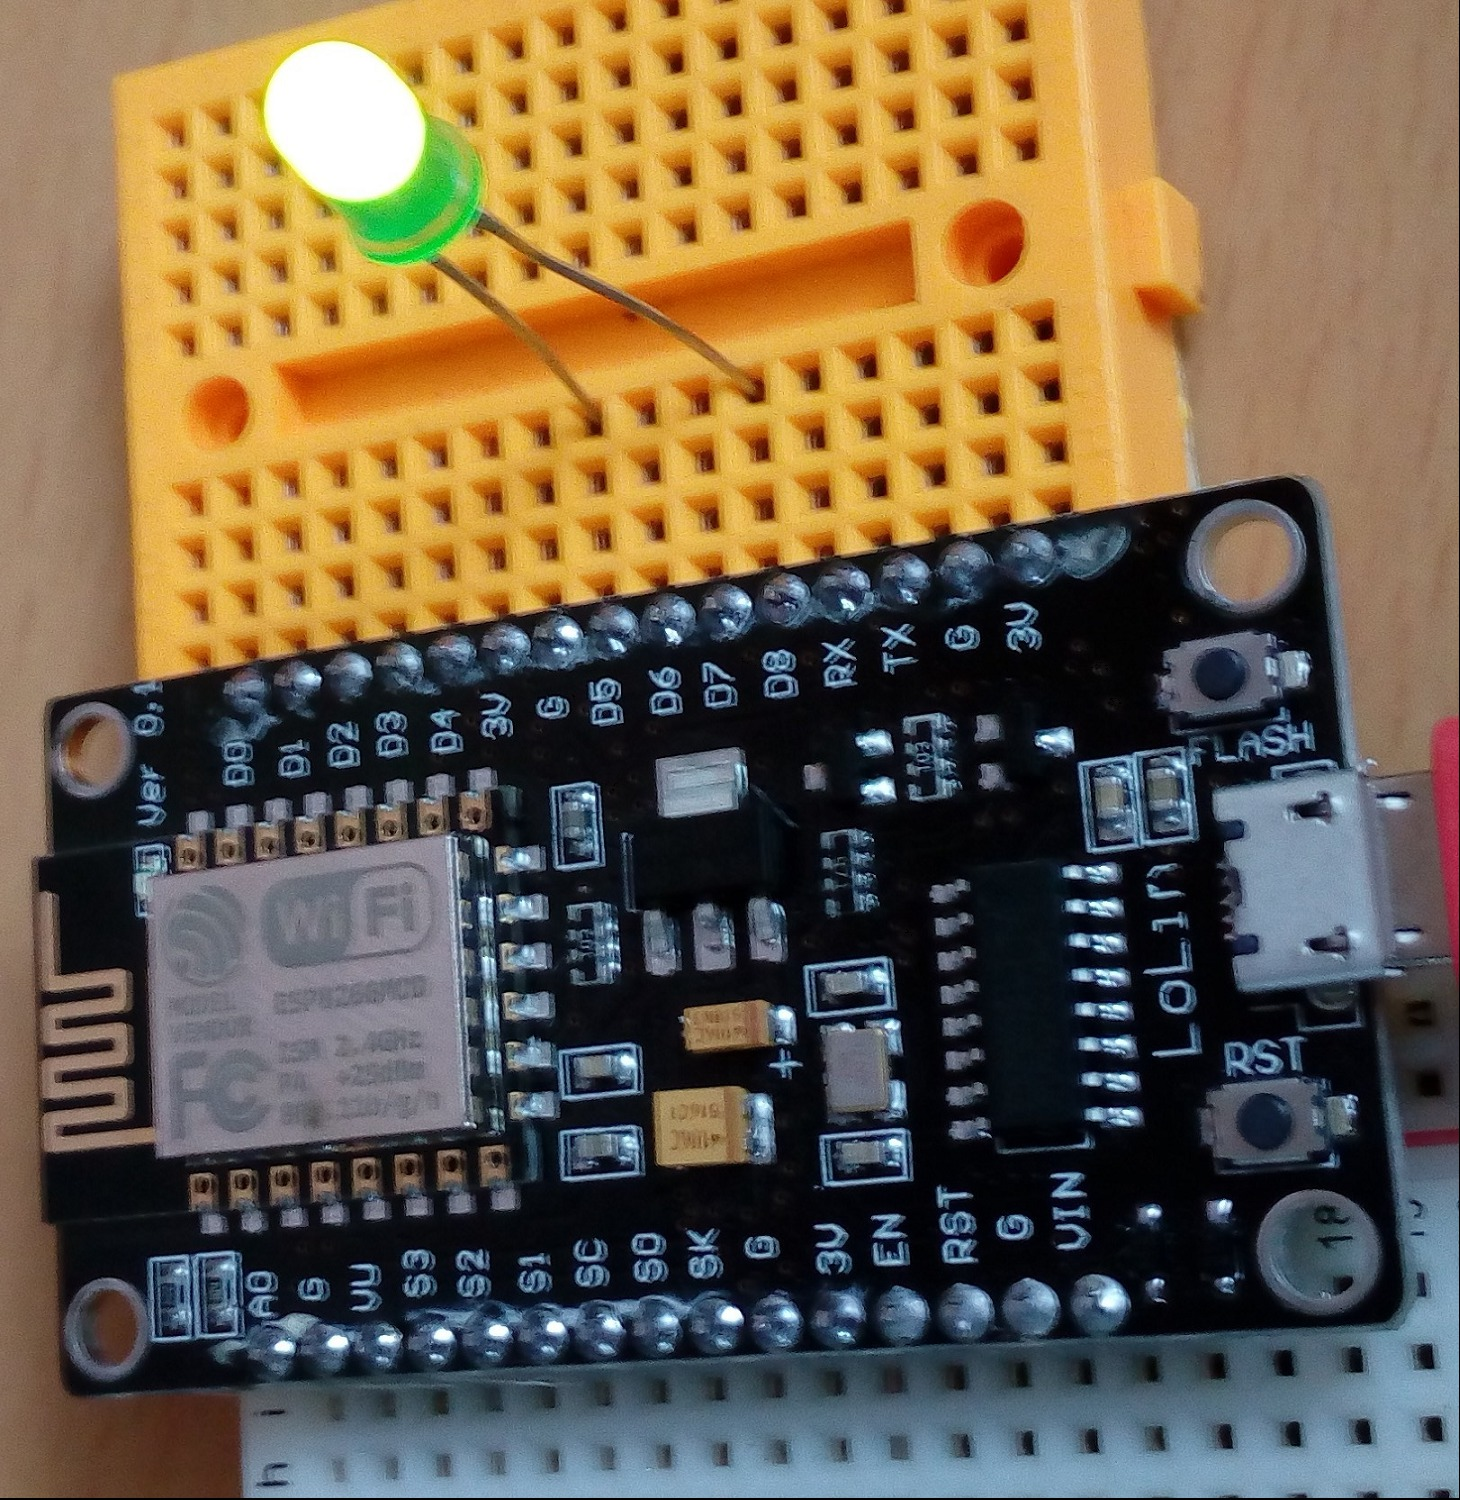
\includegraphics[width=8cm,height=8cm]{Introduction/20b.jpg}
}%
\caption{Screen Shot for LED ON and OFF}
\end{figure}
\clearpage % Start a new page
%-----------------------------------------------------------------------------------------------------
\begin{center}
\large {\textbf{Program - 1}}\\
Write a program with Arduino UNO board to calculate the distance of a obstacle based on the
Ultrasonic sensor inputs. If the distance calculated is less than a certain value turn on a buzzer / beeper with a LED in ON state and display the distance in LCD / OLED
\end{center}
\begin{flushleft}
\textbf{\textit{Components Required}}
\begin{itemize}[noitemsep,nolistsep]
\item 1 x Arduino UNO
\item 1 x Piezo Buzzer
\item 1 x LED
\item 1 x Ultrasonic Sensor HC-SR04
\item 1 x OLED (4 - Pin I2C SSD 1306)
\item 1 x Bread board
\item Jumper wires
\end{itemize}
\vspace{5mm}

\textbf{Step 1:} Download the OLED libraries from the following link and install through Arduino IDE \\
\vspace{5mm}

\textbf{\textit{Library Files}}\\ \begin{itemize}[noitemsep,nolistsep]
\item https://github.com/adafruit/Adafruit-GFX-Library
\item https://github.com/adafruit/Adafruit\_SSD1306
\end{itemize}
\vspace{5mm}

\textbf{Step 2:} Connect the components to the Arduino Uno pins as specified below  \\
Note: Refer the Fritzing for more information on connecting the components \\
\vspace{5mm}
\begin{itemize}[noitemsep,nolistsep]
    \item LED pin - 7
    \item Buzzer - 6 
    \item TRIG PIN - 13 
    \item ECHO PIN - 12 
    \item VCC (Ultrasonic) - 5V 
    \item VCC (OLED) - 5V 
    \item Ground (Common for all) - Ground above Digital pin 13
    \item SCL - A5 
    \item SDA -  A4 
\end{itemize}
\vspace{5mm}

\textbf{Step 3:} Upload the following code to the Arduino Uno using Arduino IDE \\
\vspace{5mm}

\textbf{\textit{Code}}
\begin{lstlisting}

#include <SPI.h>
#include <Wire.h>
#include <Adafruit_GFX.h>
#include <Adafruit_SSD1306.h>

//Uncomment #define ImperialNonsenseSystem for inches and Comment #define CommonSenseMetricSystem
#define CommonSenseMetricSystem
//#define ImperialNonsenseSystem

#define threshhold 30 //Change this thresshold value
#define trigPin 13
#define echoPin 12
#define buzzerPin 6
#define ledPin 7
#define OLED_RESET 4

Adafruit_SSD1306 display(OLED_RESET);

void setup() {
  Serial.begin (9600);
  pinMode(trigPin, OUTPUT);
  pinMode(echoPin, INPUT);
  pinMode(buzzerPin, OUTPUT);
  pinMode(ledPin, OUTPUT);
  display.begin(SSD1306_SWITCHCAPVCC, 0x3C); //initialize with the I2C addr 0x3C (128x64)
  display.clearDisplay();//Clear any previous values
}

void loop() {
  long duration, distance;
  
  digitalWrite(trigPin, LOW);  //PULSE ___|---|___
  delayMicroseconds(2); 
  digitalWrite(trigPin, HIGH);
  delayMicroseconds(10); 
  digitalWrite(trigPin, LOW);
  duration = pulseIn(echoPin, HIGH);
  
  #ifdef CommonSenseMetricSystem
  distance = (duration/2) / 29.1;//Conversion to centimeters
  #endif
  #ifdef ImperialNonsenseSystem
  distance = (duration/2) / 73.914;//Conversion to inches
  #endif
  
  display.setCursor(22,20);  //oled display
  display.setTextSize(3);
  display.setTextColor(WHITE);
  display.println(distance);
  display.setCursor(85,20);
  display.setTextSize(3);
  
  #ifdef CommonSenseMetricSystem
  display.println("cm");
  #endif
  #ifdef ImperialNonsenseSystem
  display.println("in");
  #endif
  
  display.display();
  if (distance>threshhold){
    digitalWrite(ledPin,HIGH);//turn on LED
    tone(buzzerPin,1000);//Send 1KHz sound signal
    delay(1000);        // ...for 1 sec
    noTone(buzzerPin);     // Stop sound...
    delay(1000);        // ...for 1sec
  }
  else{
  noTone(buzzerPin);//Stop sound
  digitalWrite(ledPin,LOW);//Turn off LED
  }
  delay(500);
  display.clearDisplay();
  Serial.println(distance);//debug
}

\end{lstlisting}
\vspace{5mm}

\textbf{\textit{Fritzing}} \\

\textbf{NOTE: Students should work on SPI with 7 pin OLED - more information on OLED with SPI. Please refer} \url{https://circuitdigest.com/article/ssd1306-oled-display}

\begin{figure}[h!]
    \centering
	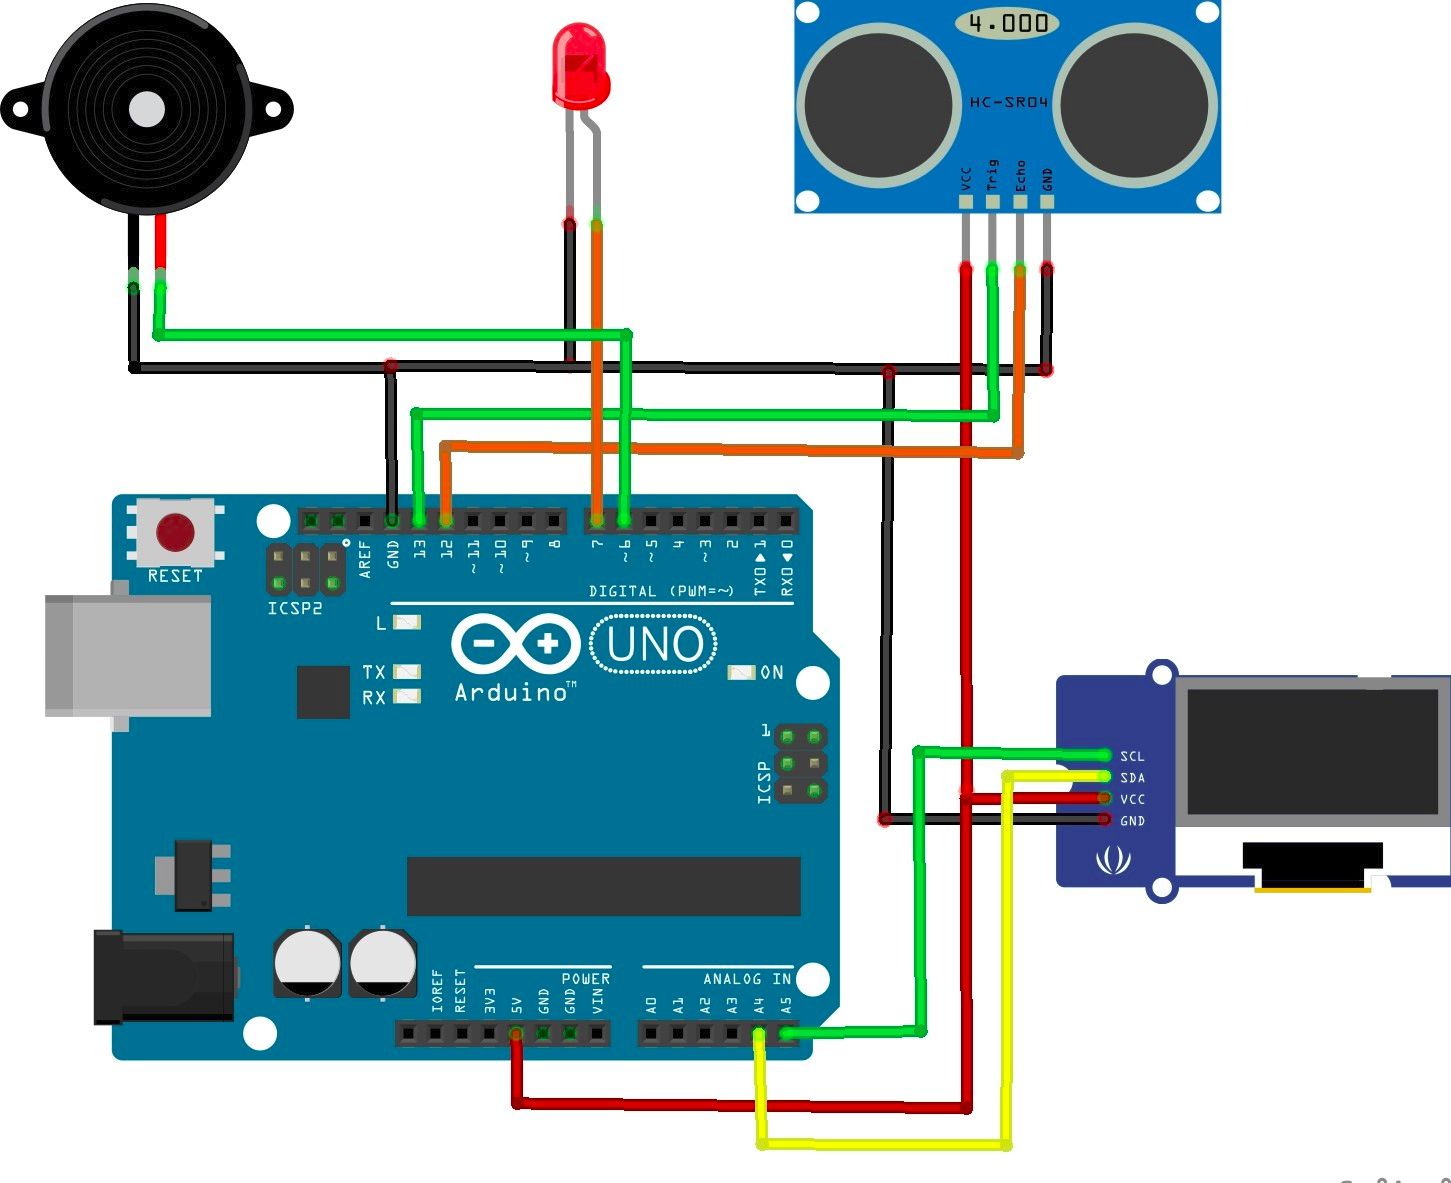
\includegraphics[width=12cm, height=10cm]{Prog1.png}
	\caption{Fritzing for Program 1}
\end{figure}
\end{flushleft}
\newpage
\begin{table}[!b]
\centering
\begin{tabular}{| >{\centering\arraybackslash}m{0.5in}| >{\arraybackslash}m{3.5in}| >{\centering\arraybackslash}m{0.8in}| >{\centering\arraybackslash}m{0.9in}|}
\hline \hline
& & &\\
\textbf{S.No}  & \hspace{1.7cm}\textbf{Rubrics for Practice Sessions} & \textbf{Max Marks} & \textbf{Marks Obtained} \\
& & &\\ \hline
1 & Physical design of circuits with devices & 2 &\\ \hline
2 & Development of Sketch/Script & 1 &\\ \hline
3 & Results & 2 &\\ \hline
4 & Clarity about the method/procedure adoption & 2 &\\ \hline
5 & Diagrams depicting connections between development boards, breadboards \& devices with Viva Voce & 3 &\\\hline
\multicolumn{2}{|c|}{} &  &\\
\multicolumn{2}{|c|}{\raggedright \textbf{\large{Total}} } & 10 &\\\hline
\multicolumn{2}{|c|}{} &  \multicolumn{2}{c|}{}\\
\multicolumn{2}{|c|}{\raggedright \textbf{\large{Signature of Faculty}} } &  \multicolumn{2}{c|}{}\\
\hline\hline
\end{tabular}
\end{table}


\clearpage
\center \textbf{Program No. 1}\vspace{11cm}

Paste your DATA SHEET here\\
\textit{[Page intentionally left blank, student to paste his/her data sheet after evaluated by the faculty in-charge] }

\clearpage
%----------------------------------------------------------------------------------------------------
\begin{center}
\large {\textbf{Program - 2}}\\
Write a program with Arduino UNO to indicate the level of temperature using the LEDs
indicating the Low, Medium \& High values of temperature (Red, Blue \& Green)
\end{center}
\begin{flushleft}

\textbf{\textit{Components Required}}
\begin{itemize}[noitemsep,nolistsep]
\item 1 x Arduino UNO
\item 1 x Blue LED
\item 1 x Red LED
\item 1 x Green LED
\item 3 x  220E Resistor (red-red-brown-gold)
\item 1 x DHT11 Temperature Sensor
\item 1 x Breadboard
\item Jumper Wires
\end{itemize}
\vspace{5mm}

\textbf{Step 1:} Download and install the Libraries for Temperature and Humidity Sensor from the following link\\
\vspace{5mm}

\textbf{\textit{Library Files}}\\ \begin{itemize}[noitemsep,nolistsep]
https://github.com/RobTillaart/Arduino/tree/master/libraries/DHTlib
\end{itemize}
\vspace{5mm}

\textbf{Step 2:} Connect the Jumper Wires as specified below \\
Note: Refer the Fritzing for more information on connecting the components \\
\vspace{5mm}

\begin{itemize}[noitemsep,nolistsep]
\item DHT DATA PIN - A0
\item Red LED - D2 
\item Blue LED - D3
\item Green LED - D4

\item Connection from the long leg of the Red LED goes to Digital Pin 2 of the Arduino Board through resistor, and another leg to the ground

\item Connection from the long leg of the Blue LED goes to Digital Pin 3 of the Arduino Board through resistor, and another leg to the ground

\item Connection from the long leg of the Green LED goes to Digital Pin 4 of the Arduino Board through resistor, and another leg to the ground

\item The VCC pin of the temperature sensor goes to 3.3v Pin of the Arduino

\item The DATA pin of the temperature sensor goes to Analog Pin A0

\item The GND of the temperature sensor goes to ground
\end{itemize}
\vspace{5mm}
\\

\textbf{Step 4:} Upload the following code to the Arduino Uno using Arduino IDE \\
\vspace{5mm}
\textbf{\textit{Code}}
\begin{lstlisting}
#include <dht.h>
dht DHT;

#define DHT11_PIN A0  //what pin we're connected to

//Variables
const int hot = 30; //set hot parameter
const int cold = 23; //set cold parameter
float hum;  //Stores humidity value
float temp; //Stores temperature value

void setup()
{
    Serial.begin(9600);
}

void loop()
{
    int chk = DHT.read11(DHT11_PIN);
    //Read data and store it to variables hum and temp
    hum = DHT.humidity;
    temp= DHT.temperature;
    //Print temp and humidity values to serial monitor
    Serial.print("Humidity: ");
    Serial.print(hum);
    Serial.print(" %");
    Serial.println("Temp: ");
    Serial.print(temp);
    Serial.println(" Celsius");
    Serial.print(temp * 1.8 + 32);// Converting to Fahrenheit
    Serial.print("  Fahrenheit");
    Serial.println("");
    if (temp < cold) { //cold
      digitalWrite(2, LOW);
      digitalWrite(3, HIGH);
      digitalWrite(4, LOW);
      Serial.println("It's Cold.");
    }
    else if (temp >= hot) { //hot
      digitalWrite(2, HIGH);
      digitalWrite(3, LOW);
      digitalWrite(4, LOW);
      Serial.println("It's Hot.");
    }
    else { //fine
    digitalWrite(2, LOW);
    digitalWrite(3, LOW);
    digitalWrite(4, HIGH);
    Serial.println("It's Fine.");
    }
    delay(10000); //Delay 10 seconds.
}
\end{lstlisting}
\textbf{\textit{Fritzing}} \\
\begin{figure}[h!]
    \centering
	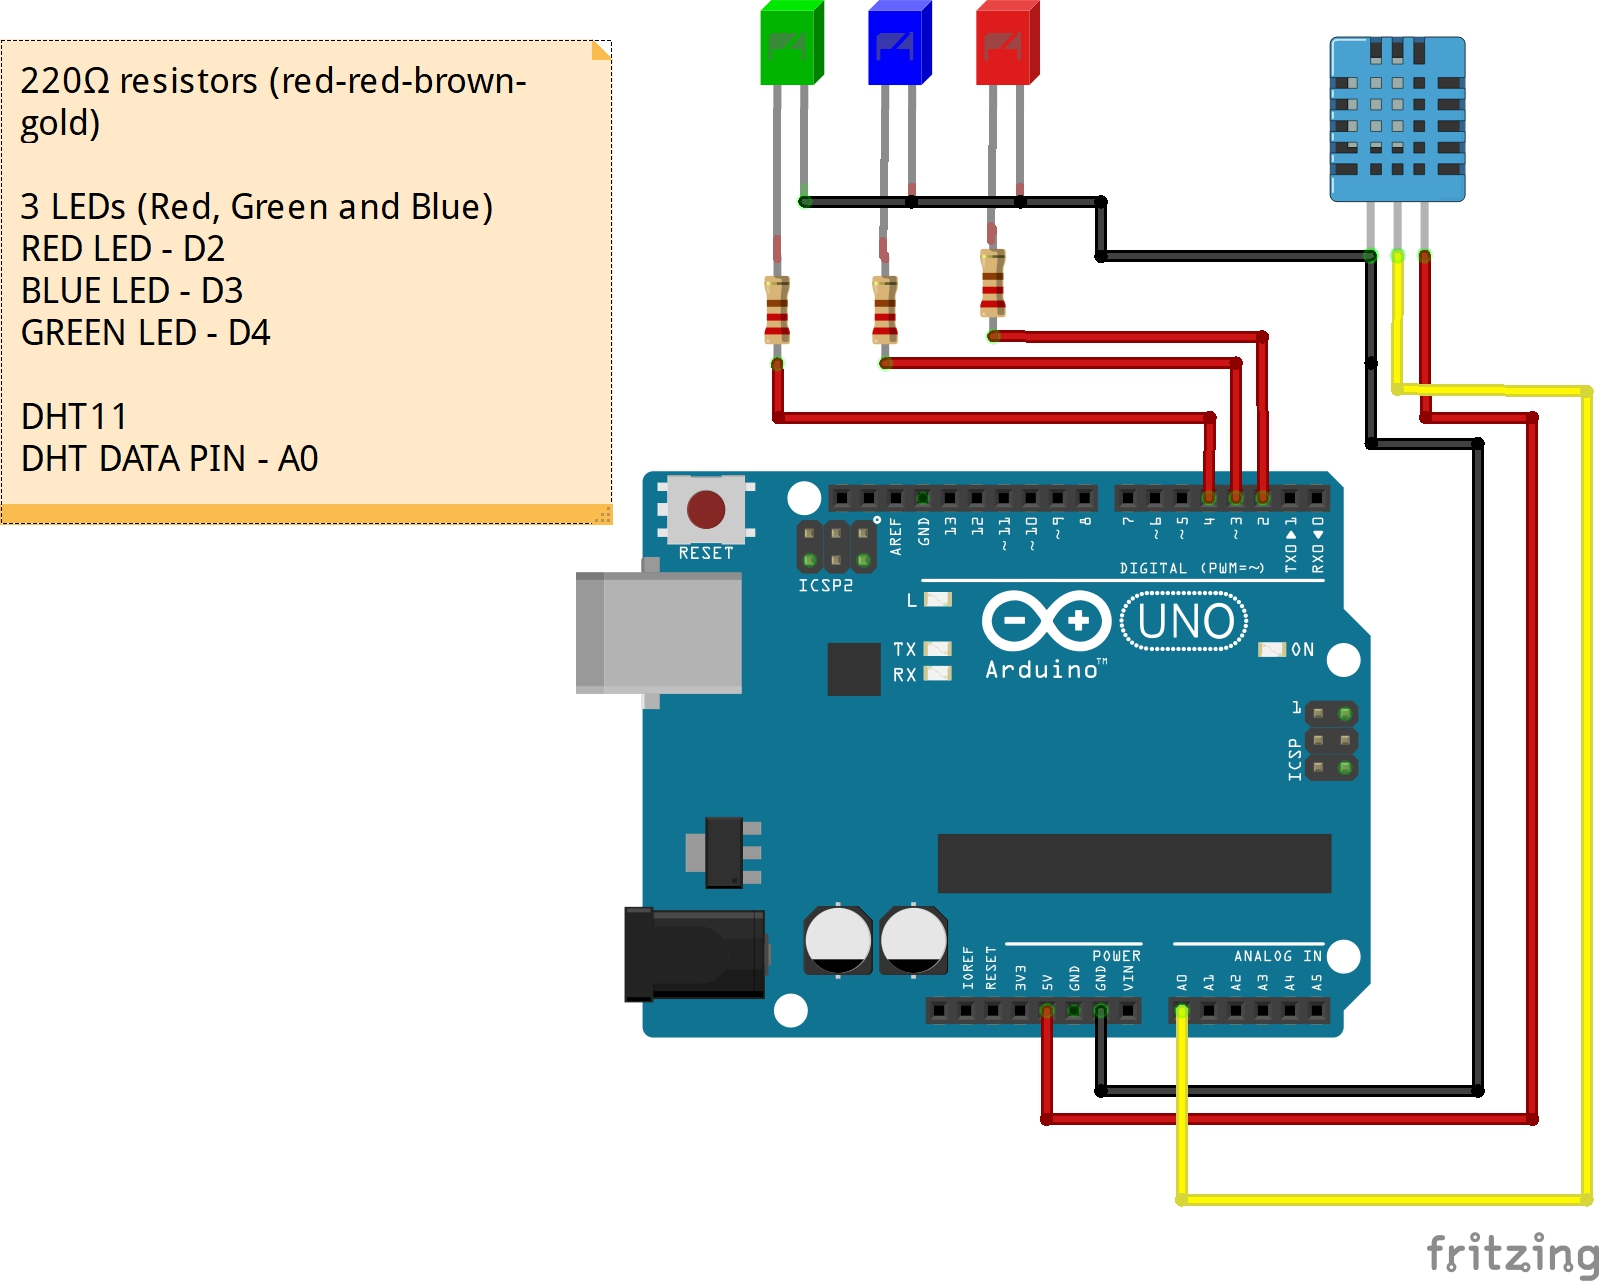
\includegraphics[width=12cm, height=10cm]{Prog2.jpg}
	\caption{Fritzing for Program 2}
\end{figure}

\textbf{\textit{Sample Output}} \\

\begin{figure}[h!]
    \centering
	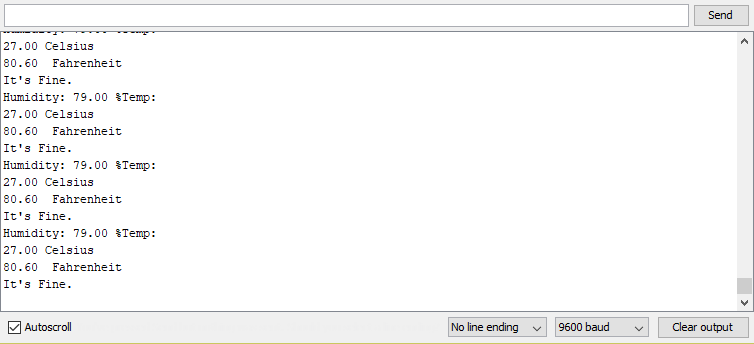
\includegraphics[width=12cm, height=6cm]{Lab2_Output.png}
	\caption{Sample Output of Program 2}
\end{figure}
\end{flushleft}\vspace{6.5cm}
\begin{table}[!b]
\centering
\begin{tabular}{| >{\centering\arraybackslash}m{0.5in}| >{\arraybackslash}m{3.5in}| >{\centering\arraybackslash}m{0.8in}| >{\centering\arraybackslash}m{0.9in}|}
\hline \hline
& & &\\
\textbf{S.No}  & \hspace{1.7cm}\textbf{Rubrics for Practice Sessions} & \textbf{Max Marks} & \textbf{Marks Obtained} \\
& & &\\ \hline
1 & Physical design of circuits with devices & 2 &\\ \hline
2 & Development of Sketch/Script & 1 &\\ \hline
3 & Results & 2 &\\ \hline
4 & Clarity about the method/procedure adoption & 2 &\\ \hline
5 & Diagrams depicting connections between development boards, breadboards \& devices with Viva Voce & 3 &\\\hline
\multicolumn{2}{|c|}{} &  &\\
\multicolumn{2}{|c|}{\raggedright \textbf{\large{Total}} } & 10 &\\\hline
\multicolumn{2}{|c|}{} &  \multicolumn{2}{c|}{}\\
\multicolumn{2}{|c|}{\raggedright \textbf{\large{Signature of Faculty}} } &  \multicolumn{2}{c|}{}\\
\hline\hline
\end{tabular}
\end{table}


\clearpage
\center \textbf{Program No. 2}\vspace{11cm}

Paste your DATA SHEET here\\
\textit{[Page intentionally left blank, student to paste his/her data sheet after evaluated by the faculty in-charge] }

\clearpage
%---------------------------------------------------------------------------------------%---------------------------------------------------------------------------------------------------------
\begin{center}
{\large {\textbf{Program - 3}}\\
Write a interactive Python Script on Raspberry Pi3 to implement the serial communication
from Raspberry Pi to Arduino and vice versa with the following components }\end{center}
{\large\begin{flushleft}{ 
a) LED \\
b) Buzzer \\
c) Temperature and Humidity Sensor  \\
d) Four Channel Relay} \\
\end{flushleft}}
\begin{flushleft}
\textbf{\textit{Components Required}}
\begin{itemize}[noitemsep,nolistsep]
\item 1 x Buzzer
\item 1 x 100 OHM Resistor for Buzzer
\item 1 x DHT11 - 3 Pin
\item 1 x Relay Switch
\item 1 x LED
\item 1 x Raspberry Pi
\item 1 x Arduino Uno
\item 1 x Breadboard
\item Jumper Wires
\end{itemize}
\vspace{5mm}

\textbf{Step 1:} Ensure that Library File for DHT11 1.2.3 is installed in Arduino\\
\vspace{5mm}

\textbf{\textit{Library Files}}\\ \begin{itemize}[noitemsep,nolistsep]
https://github.com/RobTillaart/Arduino/tree/master/libraries/DHTlib
\end{itemize}
\vspace{5mm}

\textbf{Step 2:} Connect the Jumper Wires as specified below \\
Note: Refer the Fritzing for more information on connecting the components \\
\vspace{5mm}

\begin{itemize}[noitemsep,nolistsep]
\item DHT DATA PIN - D7
\item Buzzer Positive Pin - D8
\item Led Positive Pin - D13
\item Relay Data Pin - D6

\item Connect Raspberry To Arduino Uno To Communicate With Serial Monitor
\item Connect All Sensor And Actuators To Arduino According To Circuit Diagram
\item Create A Menu Driven Python Script To Communicate To Arduino Through Serial Monitor In Raspberry Pi
\item Open Arduino Ide And Create A New Sketch
\item In Arduino IDE
        \\ Set -> Tools->Board="Arduino Uno"
        \\ Set -> Tools-> Port
\item In Python Script
        Change  Serial.Serial('<Port\_value>',9600) To Port Value Set In Arduino IDE
        Change  Baud Rate - 9600
\item In Arduino IDE
         \\ Sketch-> Include Library->Manage Library - Download Dht Sensor Library Version 1.2.3
\item Write C Code To Control Sensor And Actuators Based On Serial Monitor Request

\end{itemize}
\vspace{5mm}
\\

\textbf{Step 4:} Upload the following code to the Arduino Uno using Arduino IDE \\
\vspace{5mm}
\textbf{\textit{Code - Raspberry Pi as a Python File}}
\begin{lstlisting}
import time
import serial
ser = serial.Serial('/dev/ttyACM0', 9600)# enable the serial port and specify baud rate. To check if raspberry has detected serial port ls/dev/tty*
while True:
    ch=raw_input("1.blink \n2.buzz \n3.temeprature and humidity \n4.switch on\n5.switch off\nenter your choice")
    print("\n")
    ser.flushInput() #flush previous output
    if(ch=='1'):
        ser.write("blink")
        print("Led on ...")
        print("Led off ...")
    elif(ch=='2'):  
        ser.write("buzz")
        print("Buzzer on ...")
        print("Buzzer off ...")
    elif(ch=='3'):
        ser.write("temphumid")
        print(ser.readline()) #read the serial data sent by the UNO and print       
    elif(ch=='4'):
        ser.write("switch_on")
        print("switch on")
    elif(ch=='5'):
        ser.write("switch_off")
        print("switch off")
    else:
        print("invalid choice")
    print("\n")
\end{lstlisting}

\textbf{\textit{Code - Arduino}}
\begin{lstlisting}
#include "DHT.h"// version 1.2.3
#define DHTPIN 7    // what digital pin we're connected to
#define DHTTYPE DHT11   // DHT 22  (AM2302), AM2321
DHT dht(DHTPIN, DHTTYPE); //set dht11 - pin 7 as input
void setup() {
  Serial.begin(9600);
  pinMode(8, OUTPUT); //Set buzzer - pin 9 as an output
  pinMode(6,OUTPUT); //set switch 1 - pin 6 as output
  dht.begin();
}
void loop() {
while (Serial.available()>0) {//check if data is present in serial monitor
String ch=Serial.readString();
    //Serial.print(ch);
  if (ch=="blink") {
    digitalWrite(13, HIGH);
    delay(1000);
    digitalWrite(13, LOW);
    delay(1000);
  }
  else if(ch=="buzz"){
    tone(8, 1000); // Send 1KHz sound signal...
    delay(3000);        // ...for 1 sec
    noTone(8);     // Stop sound...
    delay(1000);        // ...for 1sec
  }
  else if(ch=="switch_on"){
    digitalWrite(6,HIGH); //close the relay circuit
    delay(1000);          //wait for 3sec
  }
  else if(ch=="switch_off"){
    digitalWrite(6,LOW);  //open the relay circuit
    delay(1000);
  }
  else if(ch=="temphumid"){
    float h = dht.readHumidity();
    float t = dht.readTemperature(); //by default celsius
    // Check if any reads failed and exit early (to try again).
    if (isnan(h) || isnan(t)) {
    Serial.println("Failed to read from DHT sensor!");
      }else{
    Serial.print("Humidity:");//print temperature and humidity in serial monitor
    Serial.print(h);
    Serial.print(" %\t");
    Serial.print("Temperature: ");
    Serial.print(t);
    Serial.println(" *C ");
      }   
      }  
      }  
      }
\end{lstlisting}
\clearpage
\textbf{\textit{Fritzing}} \\
\begin{figure}[h!]
    \centering
    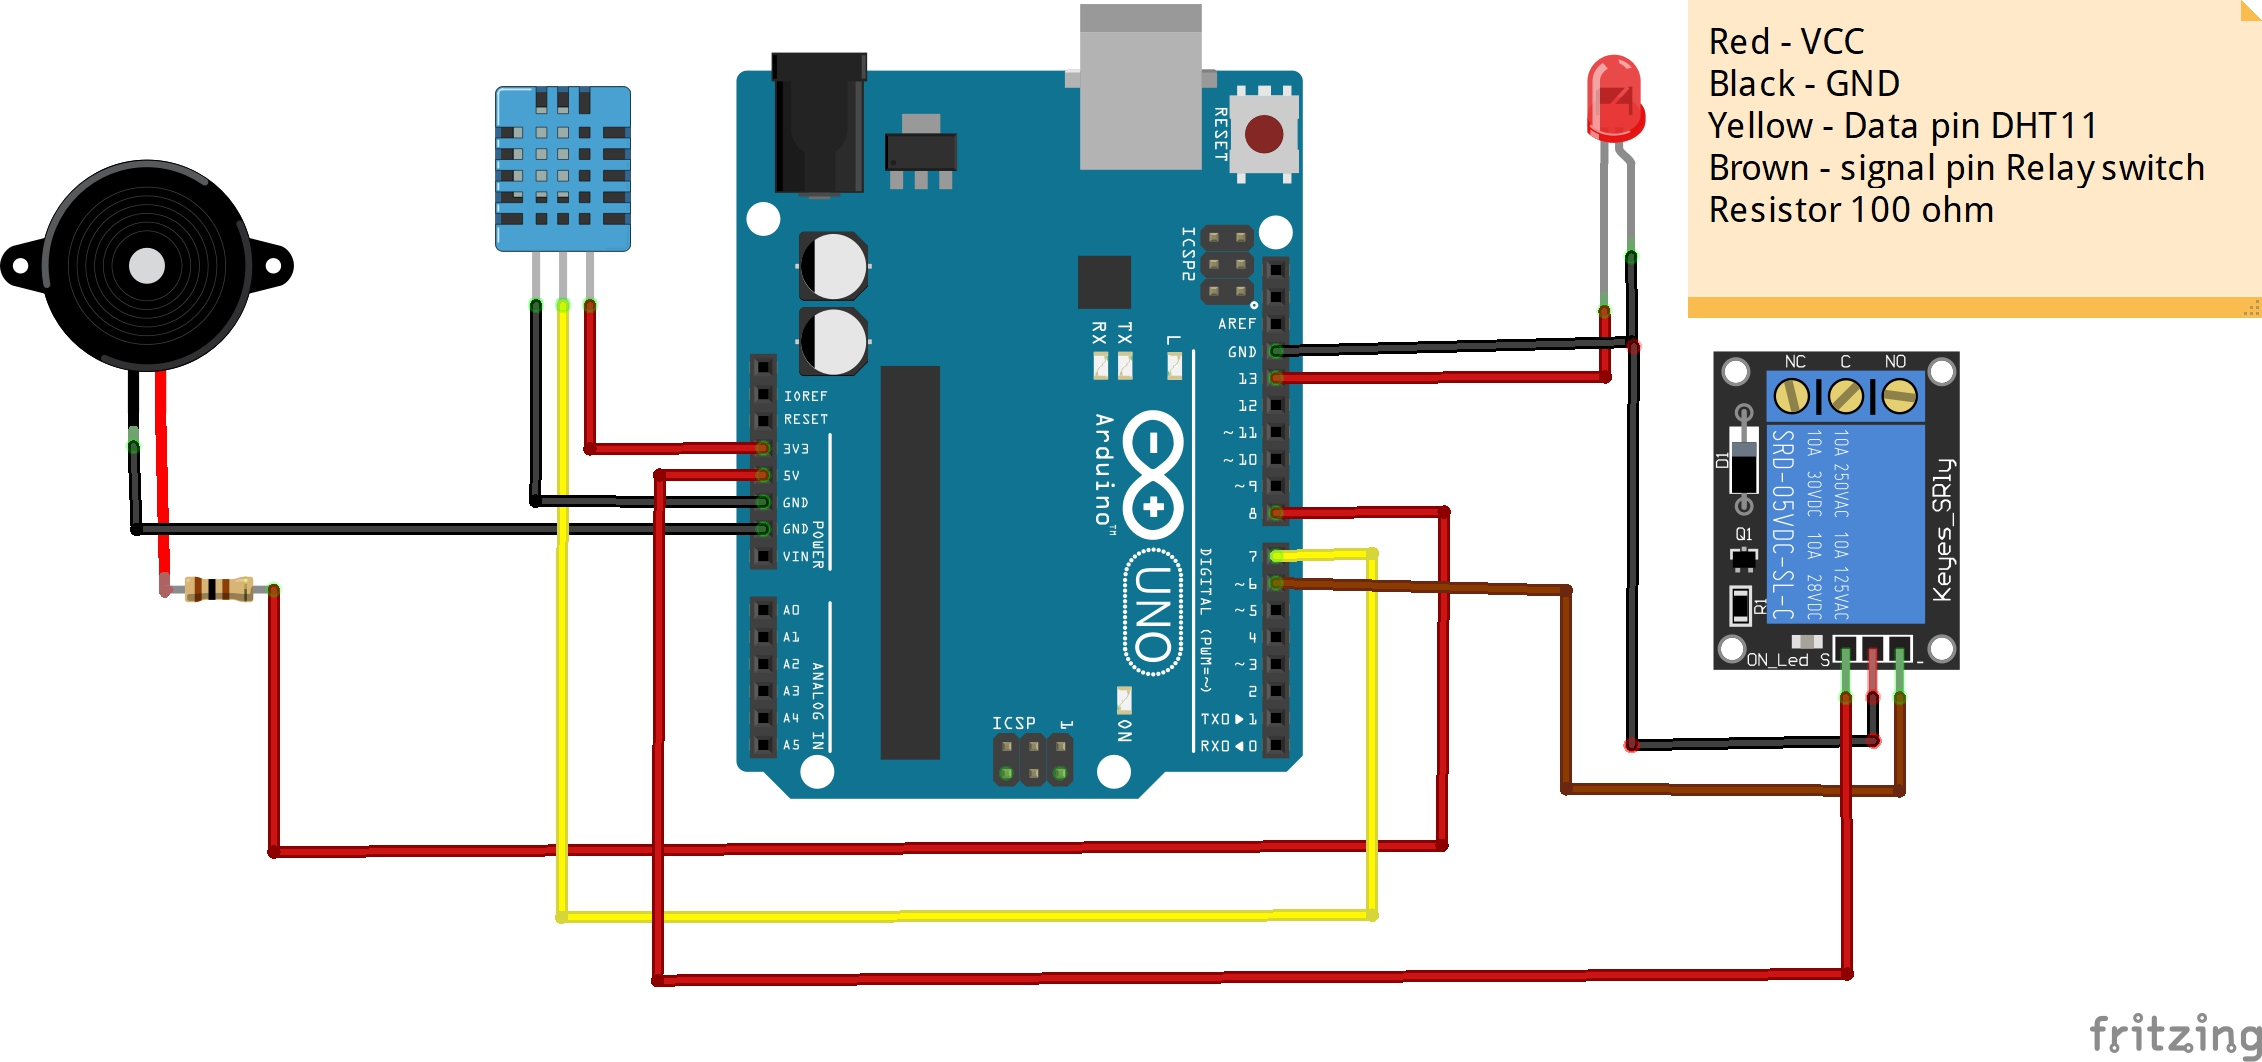
\includegraphics[width=15cm, height=8cm]{Prog3.jpg}
    \caption{Fritzing for Program 3}
\end{figure}

\textbf{\textit{Sample Output}} \\
\begin{figure}[h!]
    \centering
    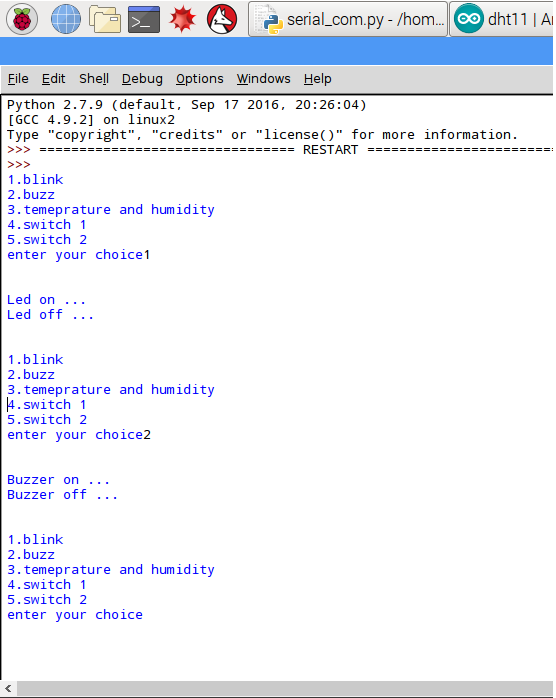
\includegraphics[width=12cm, height=9cm]{Lab3_Output_1.png}
    \caption{Sample Output of Program 3}
\end{figure}
\begin{figure}[h!]
    \centering
    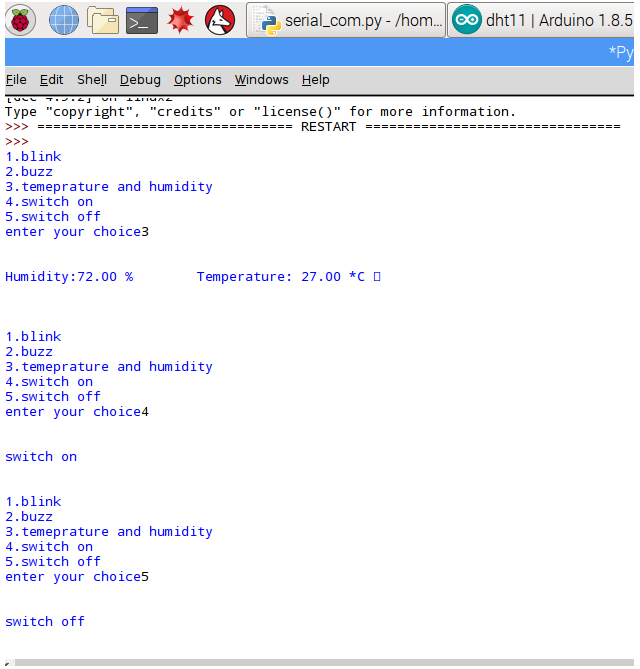
\includegraphics[width=12cm, height=9cm]{Lab3_Output_2.png}
    \caption{Sample Output of Program 3}
\end{figure}
\end{flushleft}\vspace{6.5cm}
\begin{table}[!b]
\centering
\begin{tabular}{| >{\centering\arraybackslash}m{0.5in}| >{\arraybackslash}m{3.5in}| >{\centering\arraybackslash}m{0.8in}| >{\centering\arraybackslash}m{0.9in}|}
\hline \hline
& & &\\
\textbf{S.No}  & \hspace{1.7cm}\textbf{Rubrics for Practice Sessions} & \textbf{Max Marks} & \textbf{Marks Obtained} \\
& & &\\ \hline
1 & Physical design of circuits with devices & 2 &\\ \hline
2 & Development of Sketch/Script & 1 &\\ \hline
3 & Results & 2 &\\ \hline
4 & Clarity about the method/procedure adoption & 2 &\\ \hline
5 & Diagrams depicting connections between development boards, breadboards \& devices with Viva Voce & 3 &\\\hline
\multicolumn{2}{|c|}{} &  &\\
\multicolumn{2}{|c|}{\raggedright \textbf{\large{Total}} } & 10 &\\\hline
\multicolumn{2}{|c|}{} &  \multicolumn{2}{c|}{}\\
\multicolumn{2}{|c|}{\raggedright \textbf{\large{Signature of Faculty}} } &  \multicolumn{2}{c|}{}\\
\hline\hline
\end{tabular}
\end{table}

\clearpage
\center \textbf{Program No. 3}\vspace{11cm}

Paste your DATA SHEET here\\
\textit{[Page intentionally left blank, student to paste his/her data sheet after evaluated by the faculty in-charge] }
\clearpage
%---------------------------------------------------------------------------------------%---------------------------------------------------------------------------------------------------------
\begin{center}
{\large {\textbf{Program - 4}}\\
Write a python script on Raspberry Pi to control servo motor and DC Motor based on the
potentiometer meter and button switch inputs. Also indicate the angle of the servo motor and change the color of RGB LED / Bulb}
\end{center}
\begin{flushleft}
\textbf{\textit{Components Required}}
\begin{itemize}[noitemsep,nolistsep]
\item 1 X Raspberry Pi3
\item 1 X  5v DC Motor
\item 1 X Push Button
\item 1 X  RGB LED (Common Cathode Version)
\item 1 X  100 Ohm Resistor For Red Pin
\item 1 X 120 Ohm For Green And Blue Pins
\item 1 X 10K Potentiometer
\item 1 X MCP 3008 - Analog To Digital Converter
\item 1 X 5V Servo Motor
\item 1 x Breadboard
\item Jumper Wires
\end{itemize}
\vspace{5mm}

\textbf{Step 1:} Connect the components to the Raspberry Pi3 board as specified below \\
\vspace{5mm}
\begin{itemize}[noitemsep,nolistsep]
\item Servo Motor Data Pin - Gpio 04
\item Push Button Pin - Gpio 06
\item Dc Motor Positive Pin - Gpio 13
\item LED Red Pin - GPIO 17
\item LED Green Pin - GPIO 27
\item LED Blue Pin - GPIO 22
\end{itemize}
\vspace{5mm}

\textbf{Step 2:} Connect the components to MCP3008
\begin{itemize}[noitemsep,nolistsep]
\item Clk To GPIO 16
\item DOUT To GPIO 19
\item DIN To GPIO 20
\item CS To GPIO 25
\item Potentiometer Data Pin to CH0 OG MCP3008
\end{itemize}
\vspace{5mm}

\textbf{Step 3:} Connect All Sensor And Actuators To Raspberry Pi\\
Note: Refer the Fritzing for more information on connecting the components \\\vspace{5mm}
\textbf{Step 4:} Write Python Script In Raspberry Pi To Control Sensor and Actuators \\\vspace{5mm}
\textbf{Step 5:} Run Python Script
\vspace{5mm}

\textbf{\textit{Code - Raspberry Pi as a Python File}}
\begin{lstlisting}
    from time import sleep
    import RPi.GPIO as GPIO
    GPIO.setmode(GPIO.BCM)#GPIO Numbers
    GPIO.setup(04, GPIO.OUT)#Servo motor Data pin
    GPIO.setup(06, GPIO.IN, pull_up_down=GPIO.PUD_UP)#button BOARD 31
    GPIO.setup(13, GPIO.OUT)  #DC MOTOR BOARD 33

    #RGB PIN Setup
    RED = 17 #BOARD 11
    GREEN = 27#BORAD 13
    BLUE = 22#BOARD 15

    GPIO.setup(RED,GPIO.OUT)
    GPIO.output(RED,0) #Set Default value
    GPIO.setup(GREEN,GPIO.OUT)
    GPIO.output(GREEN,0)#Set Default value
    GPIO.setup(BLUE,GPIO.OUT)
    GPIO.output(BLUE,0)#set Default value

    #MCP 8003 PINs
    CLK = 16  # BOARD 36
    DOUT = 19  # BOARD 35
    DIN = 20  # BOARD 38
    CS = 25  # BOARD 22

    #Set Up the SPI interface pins
    GPIO.setup([DIN, CLK, CS], GPIO.OUT)
    GPIO.setup(DOUT, GPIO.IN)

    # 10k trim pot connected to CH0
    potentiometer_adc = 0;
    def readadc(adcnum, clockpin, mosipin, misopin, cspin):
        if ((adcnum > 7) or (adcnum < 0)):
                return -1
        GPIO.output(cspin, True)
        GPIO.output(clockpin, False)  # start clock low
        GPIO.output(cspin, False)     # bring CS low
        commandout = adcnum
        commandout |= 0x18  # start bit + single-ended bit
        commandout <<= 3    # we only need to send 5 bits here
        for i in range(5):
                if (commandout & 0x80):
                       GPIO.output(mosipin, True)
                else:  GPIO.output(mosipin, False)
                commandout <<= 1
                GPIO.output(clockpin, True)
                GPIO.output(clockpin, False)
        adcout = 0
        # read in one empty bit, one null bit and 10 ADC bits
        for i in range(12):
                GPIO.output(clockpin, True)
                GPIO.output(clockpin, False)
                adcout <<= 1
                if (GPIO.input(misopin)):
                        adcout |= 0x1
        GPIO.output(cspin, True)
        adcout >>= 1    # first bit is 'null' so drop it
        return adcout

    def read_potentiometer():
    trim_pot = readadc(potentiometer_adc, CLK, DIN, DOUT, CS)
    #MAX Value is 1024,divide to get percentage value and Round of for 2 places
    return round(trim_pot / 1024.0, 2)

    val=[]#to store RGB values
    while True:
        #DC MOTOR BUTTON CODE
        button_state = GPIO.input(06)
        if button_state == False:#Buttom pressed
                GPIO.output(13, True)
                print('Button Pressed...')
        #       sleep(0.1)
        else:   GPIO.output(13, False)
 \end{lstlisting}
 
\textbf{Code for Potentiometer Code}
 \begin{lstlisting}
        sleep(.1)
        potentio_val=read_potentiometer()
        print(potentio_val)
        if(potentio_val<0.30):
                val=[1,0,0]     
        elif(potentio_val<0.60):
                val=[0,1,0]
        else:
                val=[0,0,1]
        GPIO.output(GREEN,val[0])
        GPIO.output(BLUE,val[1])
        GPIO.output(RED,val[2])
\end{lstlisting}

\textbf{Code for Servo Motor}

 \begin{lstlisting}
        p = GPIO.PWM(04, 50)#GPIO 4 50HZ cycle
        p.start(7.5) #duty cycle= length/period ((1.5/200)*100=7.5)
        try:
                while True:
                        p.ChangeDutyCycle(7.5)  # turn towards 90 degree
                        sleep(1) # sleep 1 second
                        p.ChangeDutyCycle(2.5)  # turn towards 0 degree
                        sleep(1) # sleep 1 second
                        p.ChangeDutyCycle(12.5) # turn towards 180 degree
                        sleep(1) # sleep 1 second
        except KeyboardInterrupt:
                p.stop()
        GPIO.cleanup()
\end{lstlisting}
\textbf{\textit{Fritzing}} \\
\begin{figure}[h!]
    \centering
	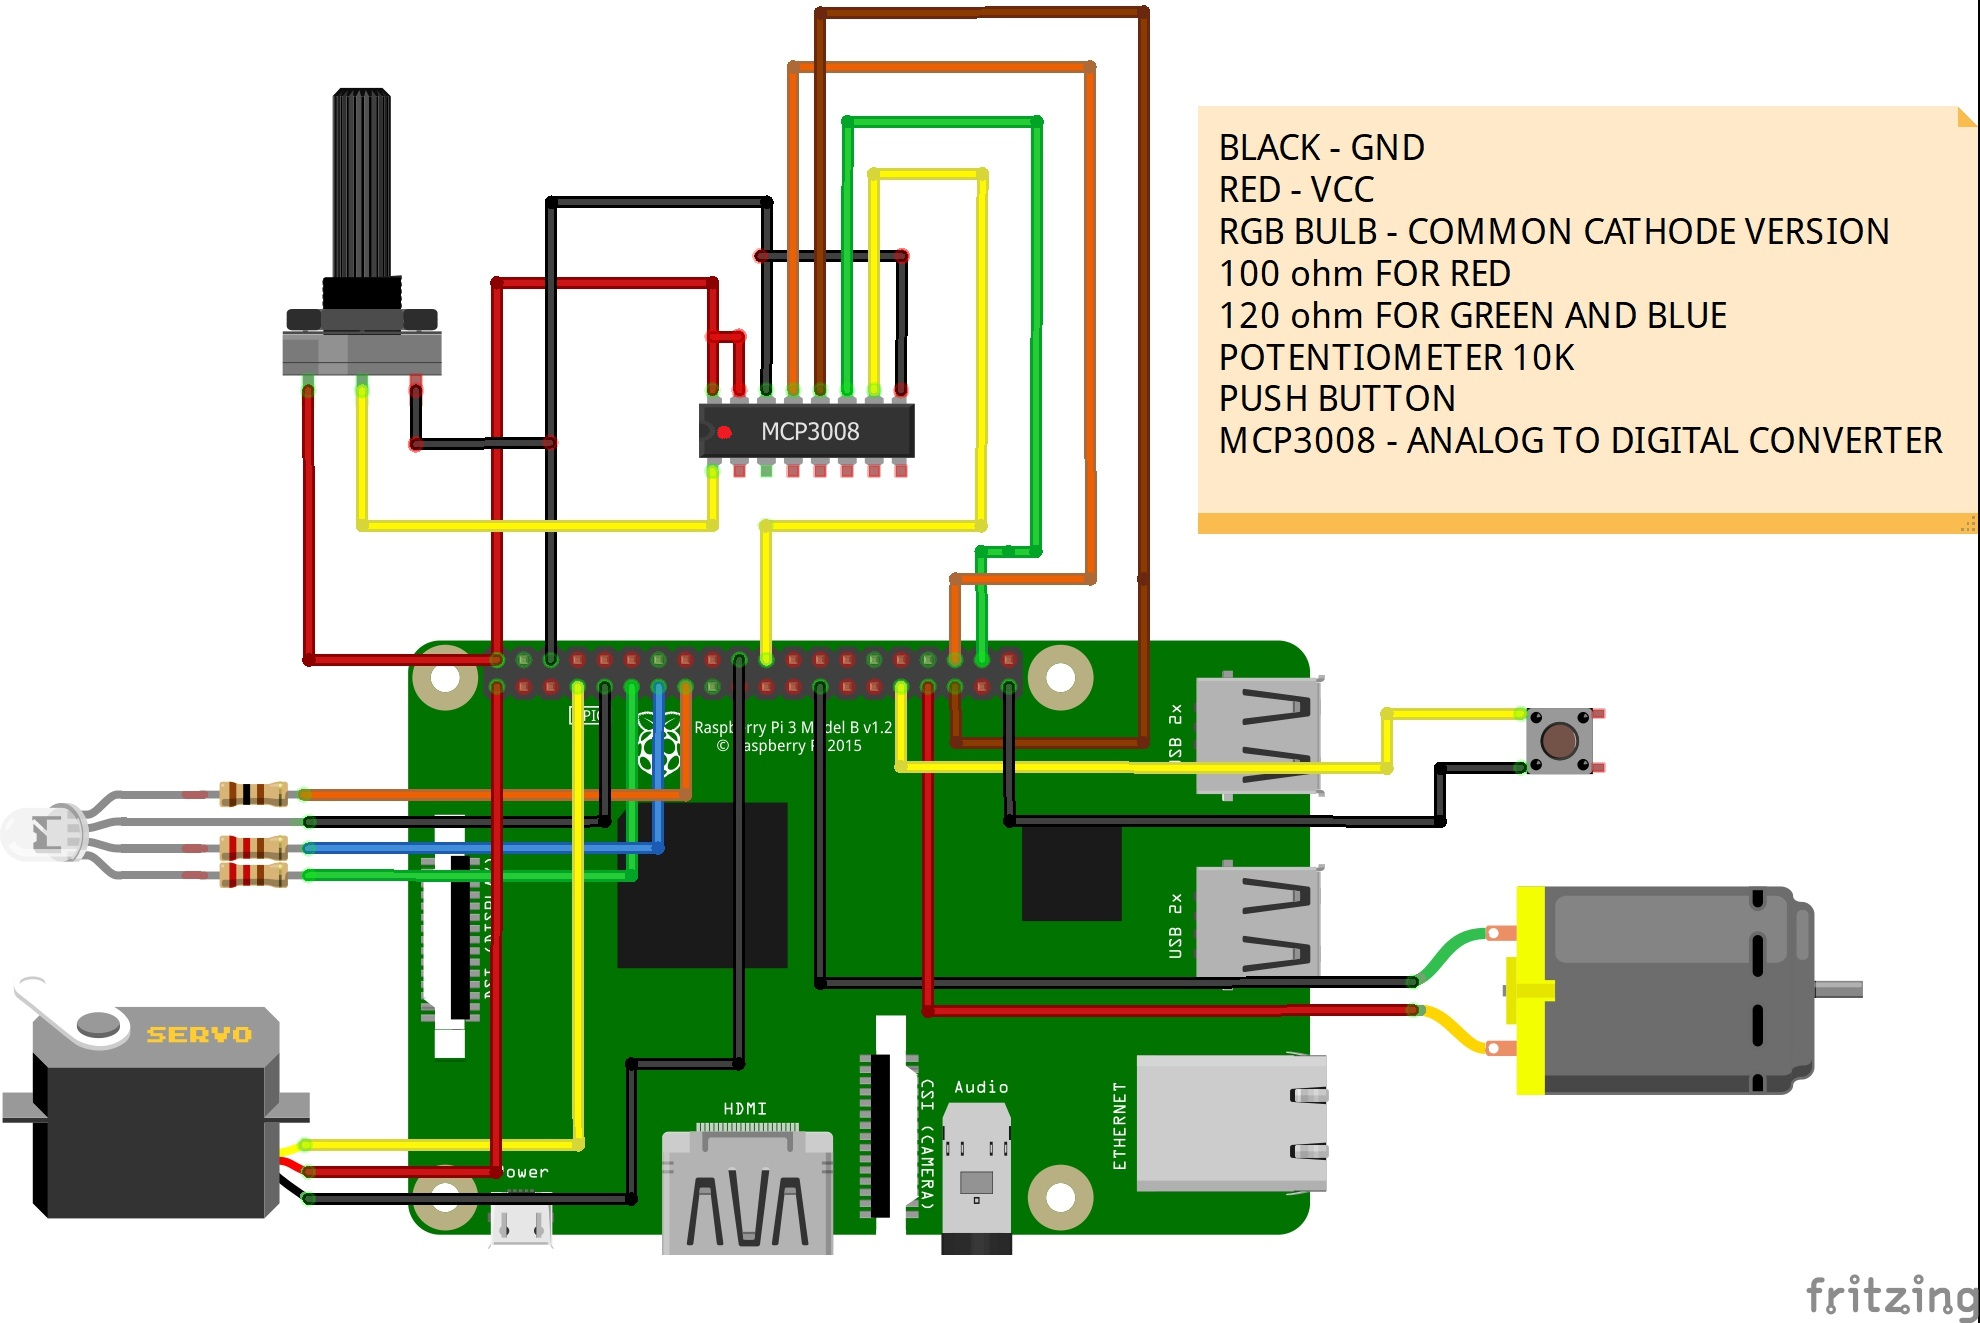
\includegraphics[width=15cm, height=8cm]{Prog4.jpg}
	\caption{Fritzing for Program 4}
\end{figure}
\textbf{\textit{ADC Converter}} \\
\begin{figure}[h!]
    \centering
	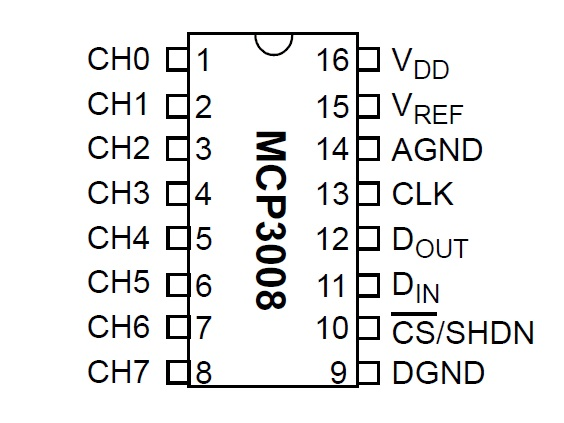
\includegraphics[width=10cm, height=6.5cm]{Lab4_ADC.jpg}
	\caption{Pin Out Diagram of ADC Converter}
\end{figure}
\end{flushleft}\vspace{6.5cm}
\begin{table}[!b]
\centering
\begin{tabular}{| >{\centering\arraybackslash}m{0.5in}| >{\arraybackslash}m{3.5in}| >{\centering\arraybackslash}m{0.8in}| >{\centering\arraybackslash}m{0.9in}|}
\hline \hline
& & &\\
\textbf{S.No}  & \hspace{1.7cm}\textbf{Rubrics for Practice Sessions} & \textbf{Max Marks} & \textbf{Marks Obtained} \\
& & &\\ \hline
1 & Physical design of circuits with devices & 2 &\\ \hline
2 & Development of Sketch/Script & 1 &\\ \hline
3 & Results & 2 &\\ \hline
4 & Clarity about the method/procedure adoption & 2 &\\ \hline
5 & Diagrams depicting connections between development boards, breadboards \& devices with Viva Voce & 3 &\\\hline
\multicolumn{2}{|c|}{} &  &\\
\multicolumn{2}{|c|}{\raggedright \textbf{\large{Total}} } & 10 &\\\hline
\multicolumn{2}{|c|}{} &  \multicolumn{2}{c|}{}\\
\multicolumn{2}{|c|}{\raggedright \textbf{\large{Signature of Faculty}} } &  \multicolumn{2}{c|}{}\\
\hline\hline
\end{tabular}
\end{table}


\clearpage
\center \textbf{Program No. 4}\vspace{11cm}

Paste your DATA SHEET here\\
\textit{[Page intentionally left blank, student to paste his/her data sheet after evaluated by the faculty in-charge] }
\clearpage
%--------------------------------------------------------------------------------------------------------------------------------------
\begin{center}
{\large {\textbf{Program - 5}}\\
Write a micro python script with esp8266 based NodeMCU board to calculate the distance of a obstacle based on the Ultrasonic sensor inputs. If the distance calculated is less than a certain value turn on a buzzer / beeper with a LED in ON state and Display the distance in LCD / OLED}
\end{center}
\begin{flushleft}
\textbf{\textit{Components Required}}
\begin{itemize}[noitemsep,nolistsep]
\item 1 x ESP8266 (Flashed with Micropython Firmware)
\item 1 x Piezo Buzzer
\item 1 x LED
\item 1 x Ultrasonic Sensor HC-SR04
\item 1 x OLED (4-pin I2C SSD 1306)
\item 1 x Breadboard with Power Supply Module
\end{itemize}
\vspace{5mm}

\textbf{Step 1:} Note: Procedure to get started with MicroPython on the ESP8266 can be found the following link \\
https://docs.micropython.org/en/latest/esp8266/esp8266/tutorial/intro.html
\vspace{5mm}

\textbf{Step 2:} Connect the components as specified below\\
Note: Refer the Fritzing for more information on connecting the components
\vspace{5mm}

\textbf{Breadboard Power Supply}
\begin{itemize}[noitemsep,nolistsep]
    \item GND of breadboard power supply to GND of ESP8266
\end{itemize}
\vspace{1mm}
\textbf{OLED}
\begin{itemize}[noitemsep,nolistsep]
    \item VCC - 3.3V(to 3V3 of ESP8266)
    \item GND - GND to common ground of Breadboard Power Supply
    \item SCL - D1(GPIO5)
    \item SDA - D2
\end{itemize}
\vspace{1mm}
\textbf{Ultrasonic Sensor}
\begin{itemize}[noitemsep,nolistsep]
    \item VCC - VCC to 5V + of Breadboard Power Supply
    \item GND - to common ground of Breadboard Power Supply
    \item Trig - D3(GPIO0)
    \item Echo - D4(GPIO2)
\end{itemize}

\textbf{Buzzer}
\begin{itemize}[noitemsep,nolistsep]
    \item + to D8(GPIO15)
    \item - to common ground of Breadboard Power Supply
\end{itemize}
\vspace{1mm}
\textbf{LED}
\begin{itemize}[noitemsep,nolistsep]
    \item + to D7(GPIO13)
    \item - to common ground of Breadboard Power Supply
\end{itemize}
\clearpage

\textbf{\textit{Code}}
\begin{lstlisting}
from machine import I2C,Pin
import time
import ssd1306
import sys
import machine
import utime
threshhold = 50
i2c = I2C(-1,Pin(5),Pin(4))
led = Pin(13,Pin.OUT)
led.off()
buzz = Pin(15,Pin.OUT)
buzz.off()
display = ssd1306.SSD1306_I2C(128,64,i2c)
display.fill(0)
display.text('Experiment',30,0)
display.text('Loading',50,10)
display.show()
utime.sleep(5)
while True:
	trig=machine.Pin(0, machine.Pin.OUT)
	trig.off()
	utime.sleep_us(2)
	trig.on()
	utime.sleep_us(10)
	trig.off()
	echo=machine.Pin(2, machine.Pin.IN)
	while echo.value() == 0:
		pass
	t1 = utime.ticks_us()
	while echo.value() == 1:
		pass
	t2 = utime.ticks_us()
	cm = (t2 - t1) / 58.0
	print(cm)
	display.fill(0)
	display.text(str(cm),30,0)
	if cm > threshhold:
		display.text('Threshhold Value',1,30)
		led.on()
		buzz.on()
	else:
		display.text('Value OK',1,30)
		led.off()
		buzz.off()
	display.show()
	utime.sleep(2)
\end{lstlisting}
\textbf{\textit{Fritzing}} \\
NOTE: Students should work on SPI with 7 pin OLED - more information on OLED with SPI.
Please refer https://circuitdigest.com/article/ssd1306-oled-display
\begin{figure}[h!]
    \centering
	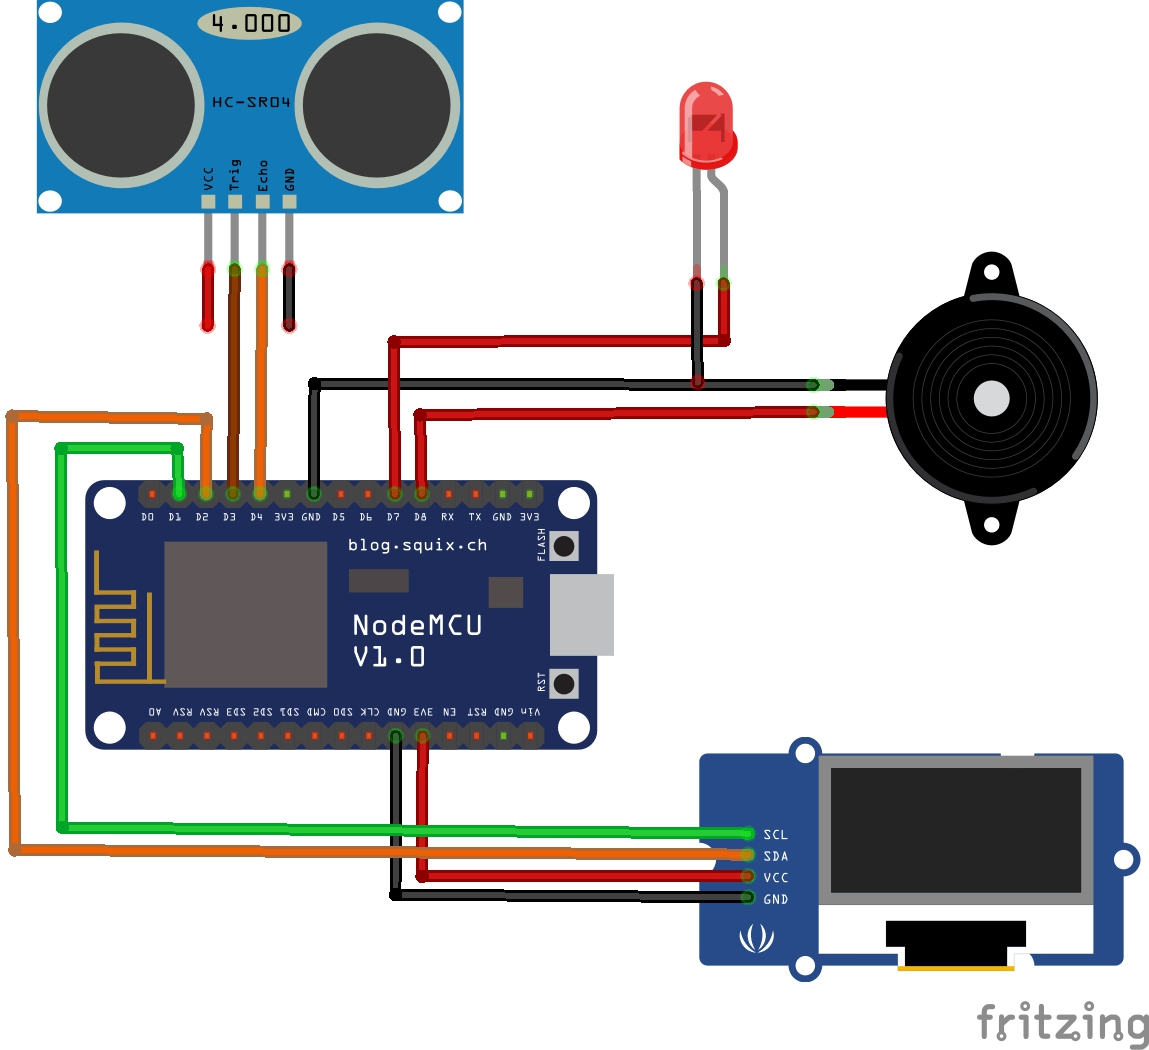
\includegraphics[width=10cm, height=7cm]{Prog5.jpg}
	\caption{Fritzing for Program 5}
\end{figure}
\vspace{3mm}

\textbf{\textit{ESP8266 - NodeMCU}} \\
\begin{figure}[h!]
    \centering
	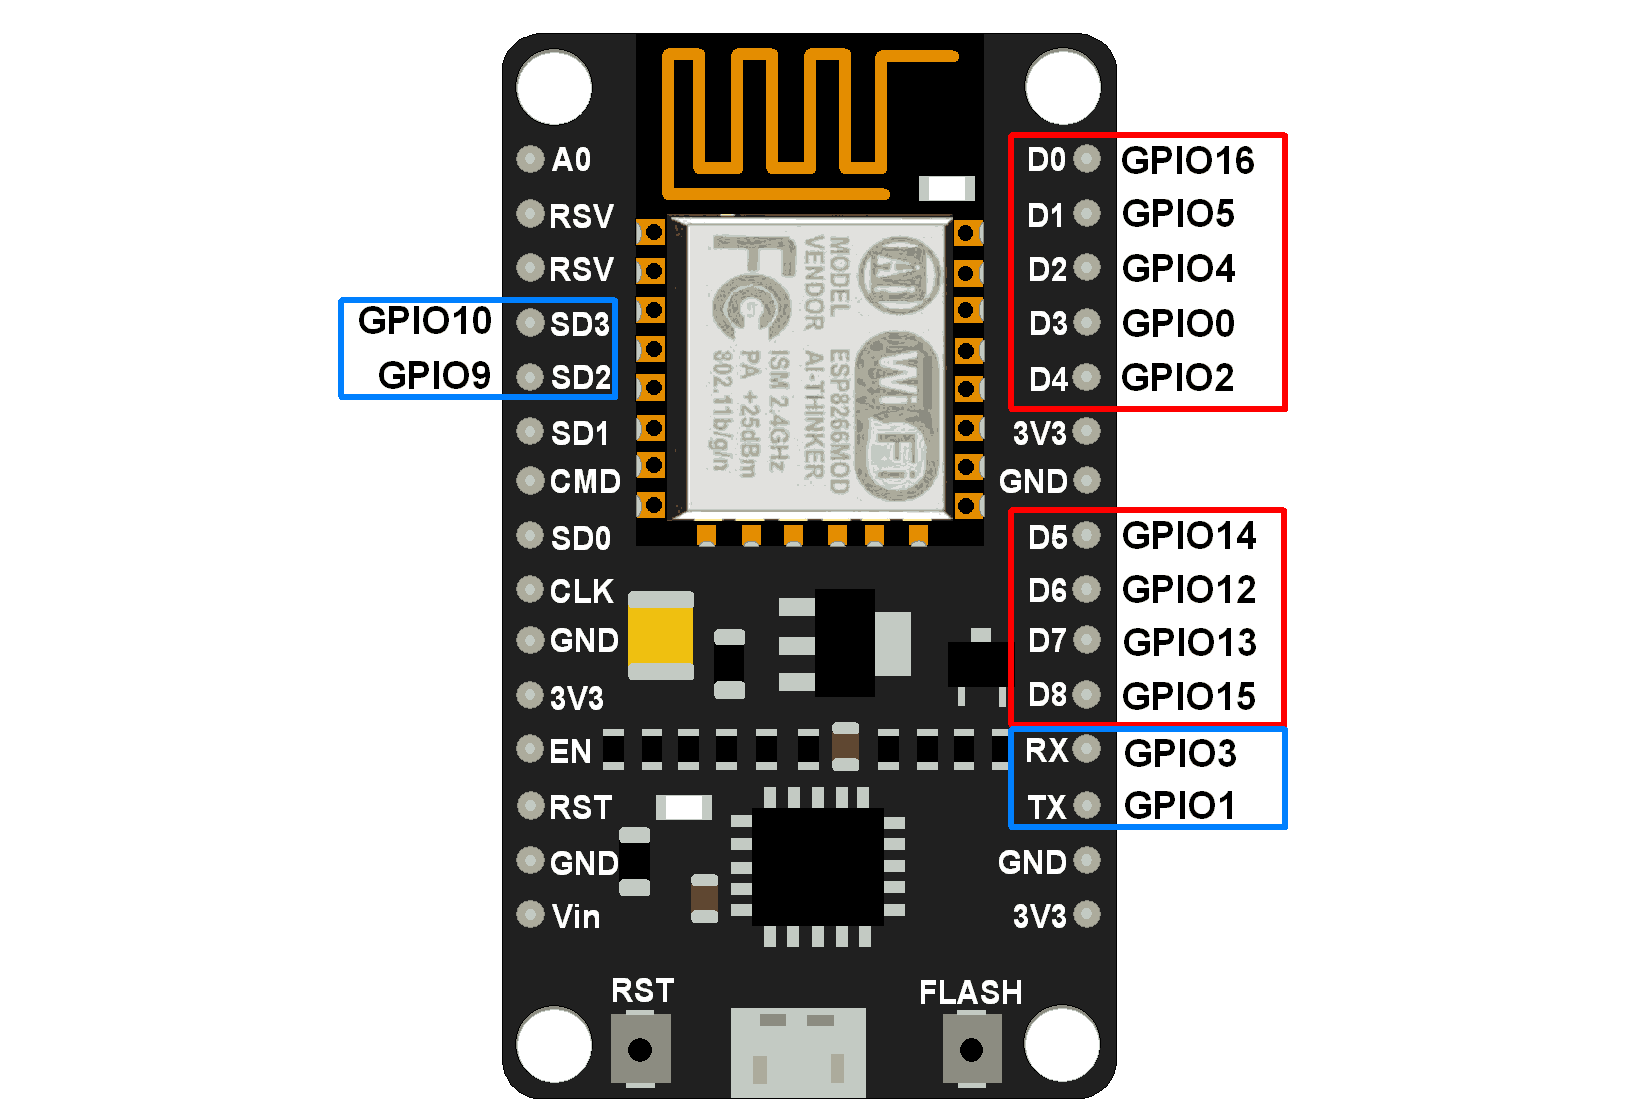
\includegraphics[width=8cm, height=5cm]{Lab5.png}
	\caption{Pin Out Diagram ESP8266 based NodeMCU}
\end{figure}
\end{flushleft}\vspace{6.5cm}
\begin{table}[!b]
\centering
\begin{tabular}{| >{\centering\arraybackslash}m{0.5in}| >{\arraybackslash}m{3.5in}| >{\centering\arraybackslash}m{0.8in}| >{\centering\arraybackslash}m{0.9in}|}
\hline \hline
& & &\\
\textbf{S.No}  & \hspace{1.7cm}\textbf{Rubrics for Practice Sessions} & \textbf{Max Marks} & \textbf{Marks Obtained} \\
& & &\\ \hline
1 & Physical design of circuits with devices & 2 &\\ \hline
2 & Development of Sketch/Script & 1 &\\ \hline
3 & Results & 2 &\\ \hline
4 & Clarity about the method/procedure adoption & 2 &\\ \hline
5 & Diagrams depicting connections between development boards, breadboards \& devices with Viva Voce & 3 &\\\hline
\multicolumn{2}{|c|}{} &  &\\
\multicolumn{2}{|c|}{\raggedright \textbf{\large{Total}} } & 10 &\\\hline
\multicolumn{2}{|c|}{} &  \multicolumn{2}{c|}{}\\
\multicolumn{2}{|c|}{\raggedright \textbf{\large{Signature of Faculty}} } &  \multicolumn{2}{c|}{}\\
\hline\hline
\end{tabular}
\end{table}


\clearpage
\center \textbf{Program No. 5}\vspace{11cm}

Paste your DATA SHEET here\\
\textit{[Page intentionally left blank, student to paste his/her data sheet after evaluated by the faculty in-charge] }
\clearpage
%--------------------------------------------------------------------------------------------------------------------------------------
\begin{center}
{\large {\textbf{Program - 6}}\\
Write a micro Python Script with ESP8266 based NodeMCU board to operate a 4 Channel Relay demonstrating minimal home automation}
\end{center}
\begin{flushleft}

\textbf{\textit{Introduction}}
\justify{Building Smart Switch Box experiment is a demonstration of building a smart switch box controlling the devices connected to them through internet using dashboard via NodeMCU Wi-Fi device using relays. The device and the dashboard interaction is done through a protocol called Message Queuing Telemetry Transport [MQTT].}
\vspace{5mm}

\justify{
\textbf{\textit{Working Process of MQTT}}\\
MQTT is a lightweight publish/subscribe messaging protocol designed for M2M (machine to machine) telemetry in low bandwidth environments. Telemetry is a process of recording and transmitting the readings of an instrument\\
\\
Clients do not have addresses like in email systems, and messages are not sent to clients. Instead messages are \textbf{published to broker on a topic}. The job of an MQTT broker is to filter messages based on topic and then distribute them to subscribers. A client can receive these messages by subscribing to that topic on the same broker. In this model there is \textbf{no direct connection} between a publisher and subscriber.}
\\
\vspace{2mm}

\begin{figure}[h!]
    \centering
	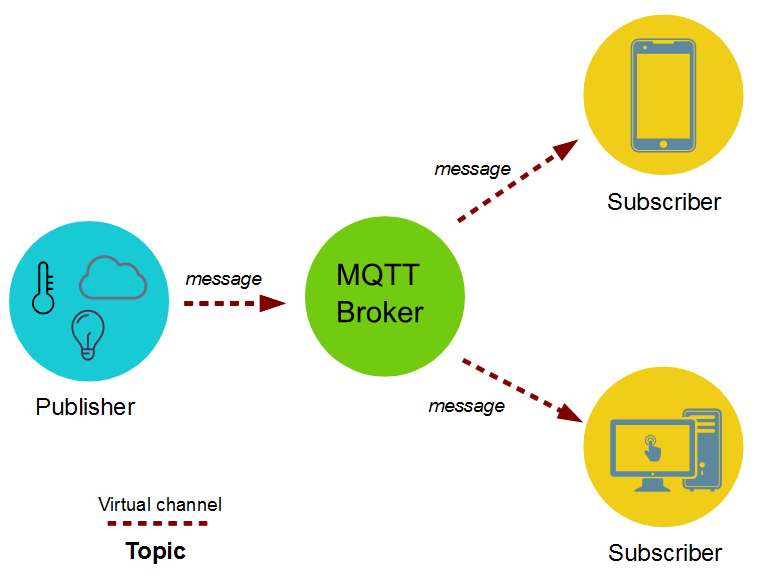
\includegraphics[width=12cm, height=9cm]{Prog10/0.png}
	\caption{MQTT - Publish and Subscribe Model}
\end{figure}
\vspace{2mm}
\clearpage

\justify{
\textbf{\textit{Topics – MQTT Addressing}}\\
These are like channels in the TV radio model. Topics are what connects the publisher and subscriber. In MQTT there is no formal structure and a publisher is free to choose its own topic names and structure.} \\
\justify{
\textbf{\textit{MQTT Broker Connections}}\\
MQTT uses TCP/IP to connect to the broker. TCP is a connection orientated protocol with error correction and guarantees that packets are received in order.
    However that does not mean that messages cannot be lost.} \\
\justify{
\textbf{\textit{MQTT Clients}}\\
    Because MQTT clients do not have addresses like email addresses, phone numbers etc. The programmers do not need to assign addresses to clients like you do with most messaging systems.}\\
\justify{
\textbf{\textit{MQTT Brokers or Servers}}\\
Note: The original term was broker but it has now been standardized as Server. You will see both terms used.\\
There are many MQTT brokers available that you can use for testing and for real applications. There are free self hosted brokers, the most popular being Mosquitto and commercial ones like HiveMQ.}\\
\justify{
\textbf{\textit{Components Required}}}
\begin{itemize}[noitemsep,nolistsep]
    \item NodeMCU (esp8266)
    \item 4 Channel Relay
    \item 5v-3v Power Supply
    \item Bread board
    \item Jumper Wires, Bulbs
    \item Internet with SSID, password
\end{itemize}
\justify{
\textbf{\textit{Procedure}}}
 \begin{enumerate}[noitemsep,nolistsep]
     \item Build the Switch Box Wiring
     \item Build the Smart Box Circuit - with NodeMCU and 4 - Channel Relay Board
     \item NodeMCU configuration - using Arduino IDE  [flashing NodeMCU]
     \item Dashboard Setup
     \item Parameters Configuration - Program
     \item Execution of Smart Switch Box
 \end{enumerate}
\justify{\textbf{Step 1:} Building the Switch Box Wiring}

\begin{figure}[h!]
    \centering
	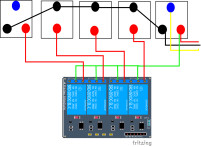
\includegraphics[width=9cm, height=6cm]{Prog10/1.jpg}	
	\caption{Wiring Diagram of Power Extension Box with 4 Relay Board}
\end{figure}
\vspace{5mm}


\begin{figure}[h!]
    \centering
	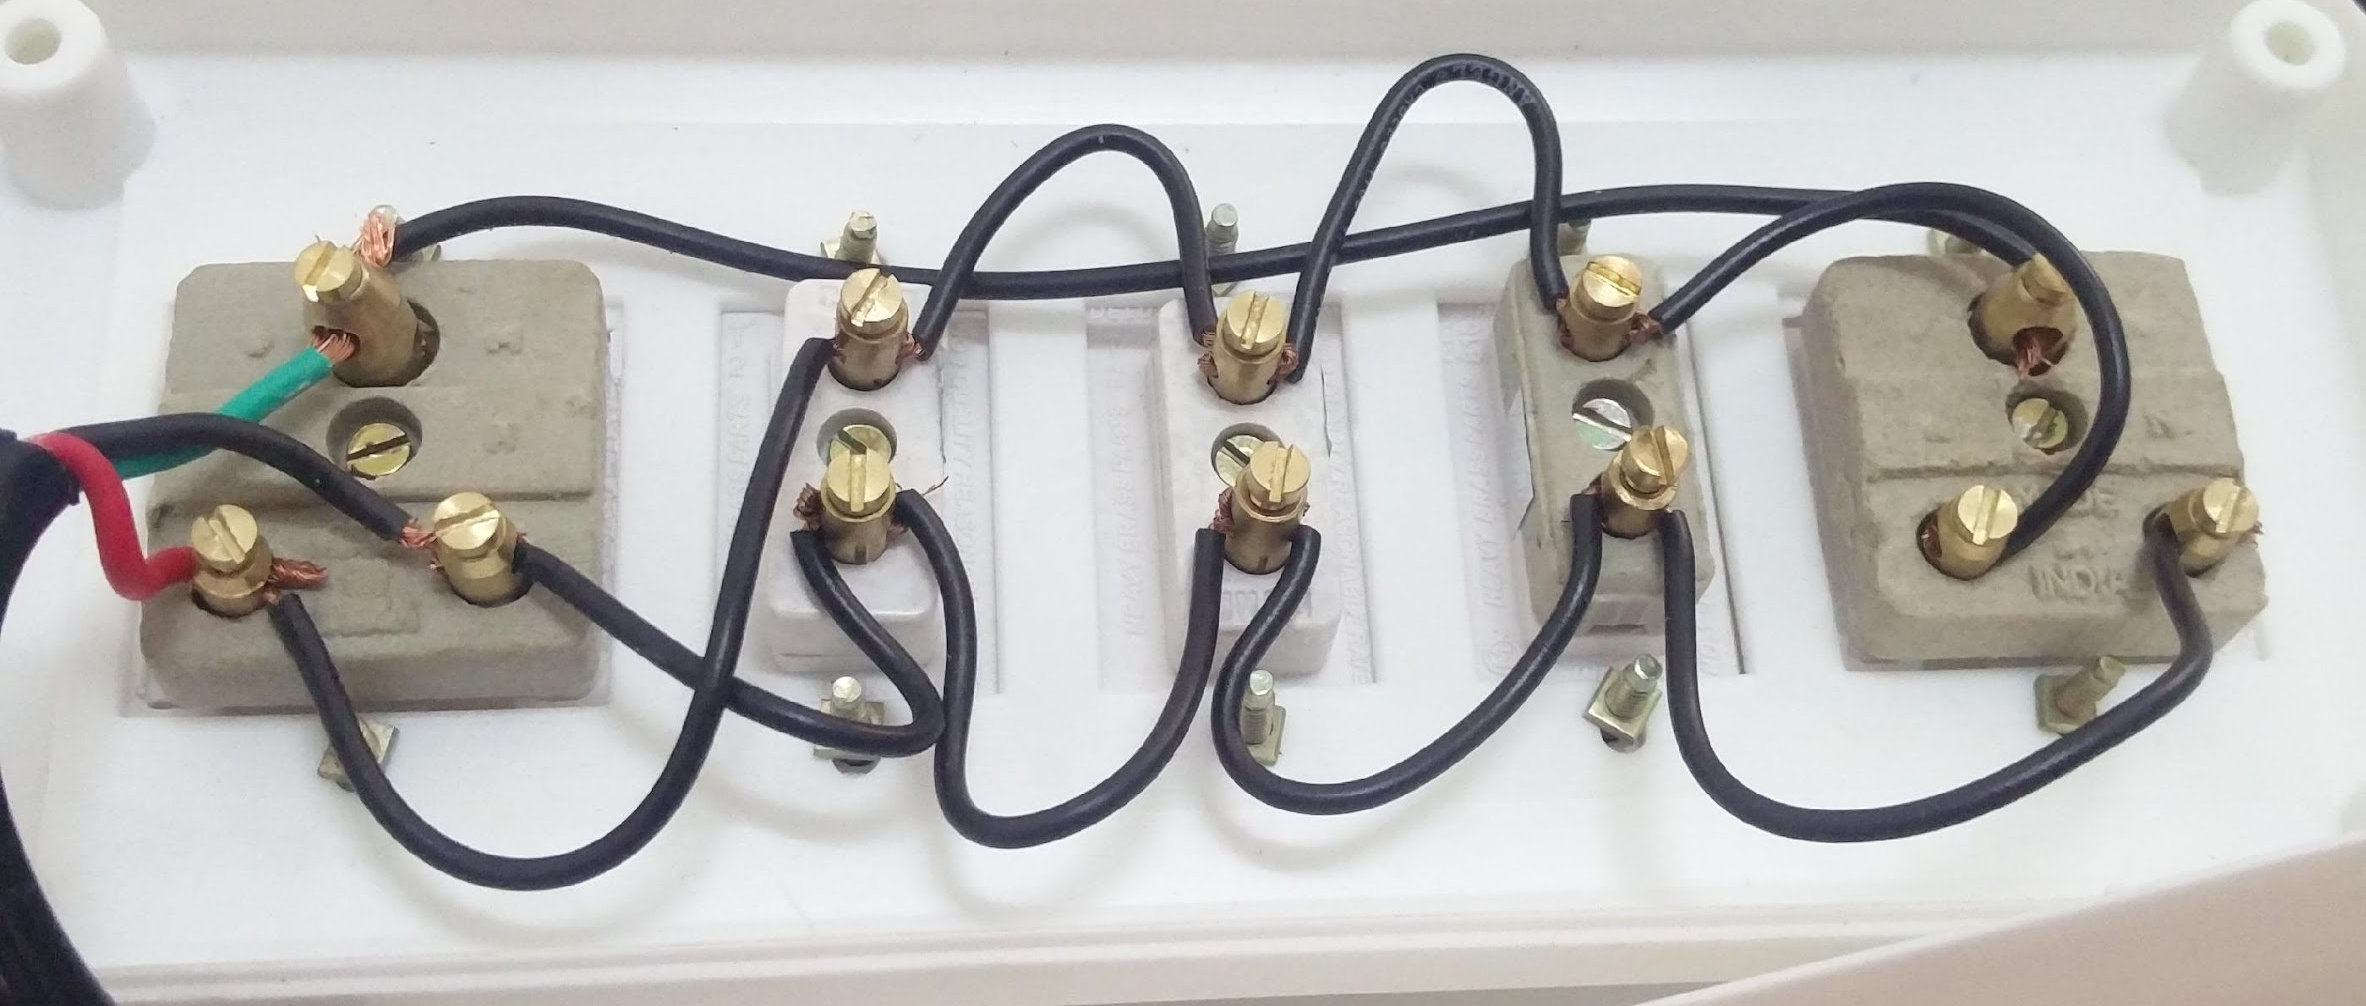
\includegraphics[width=10cm, height=7cm]{Prog10/2.jpg}
	\caption{Original Switch Box Wiring}
\end{figure}
\vspace{5mm}

\begin{figure}[h!]
    \centering
	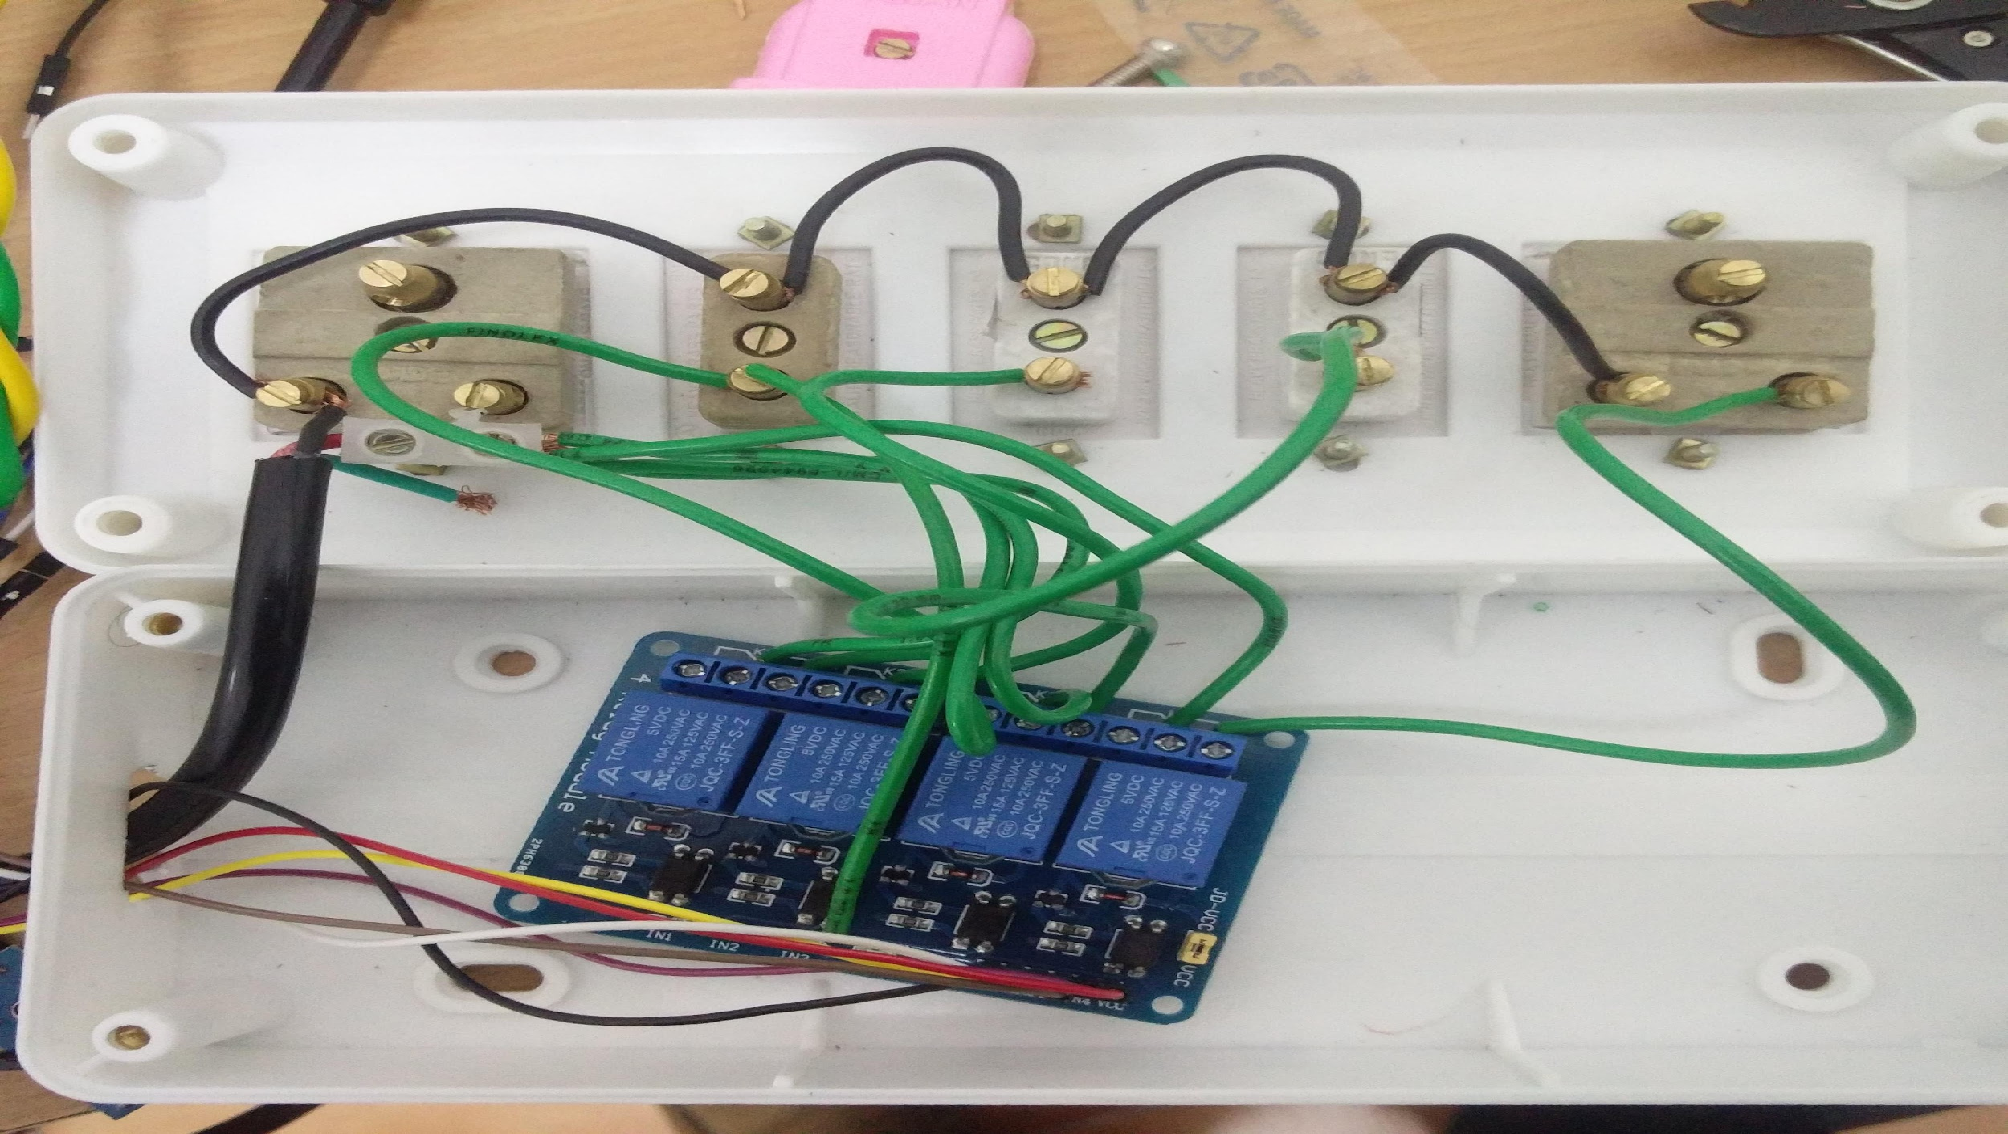
\includegraphics[width=10cm, height=6cm]{Prog10/3.png}
	\caption{Modified Switch Box Wiring with 4 Channel Relay}
\end{figure}
\vspace{5mm}

\justify{\textbf{Step 2}: Build the Smart Box circuit \\
     With NodeMCU and 4-Channel Relay Board }

\begin{figure}[h!]
    \centering
	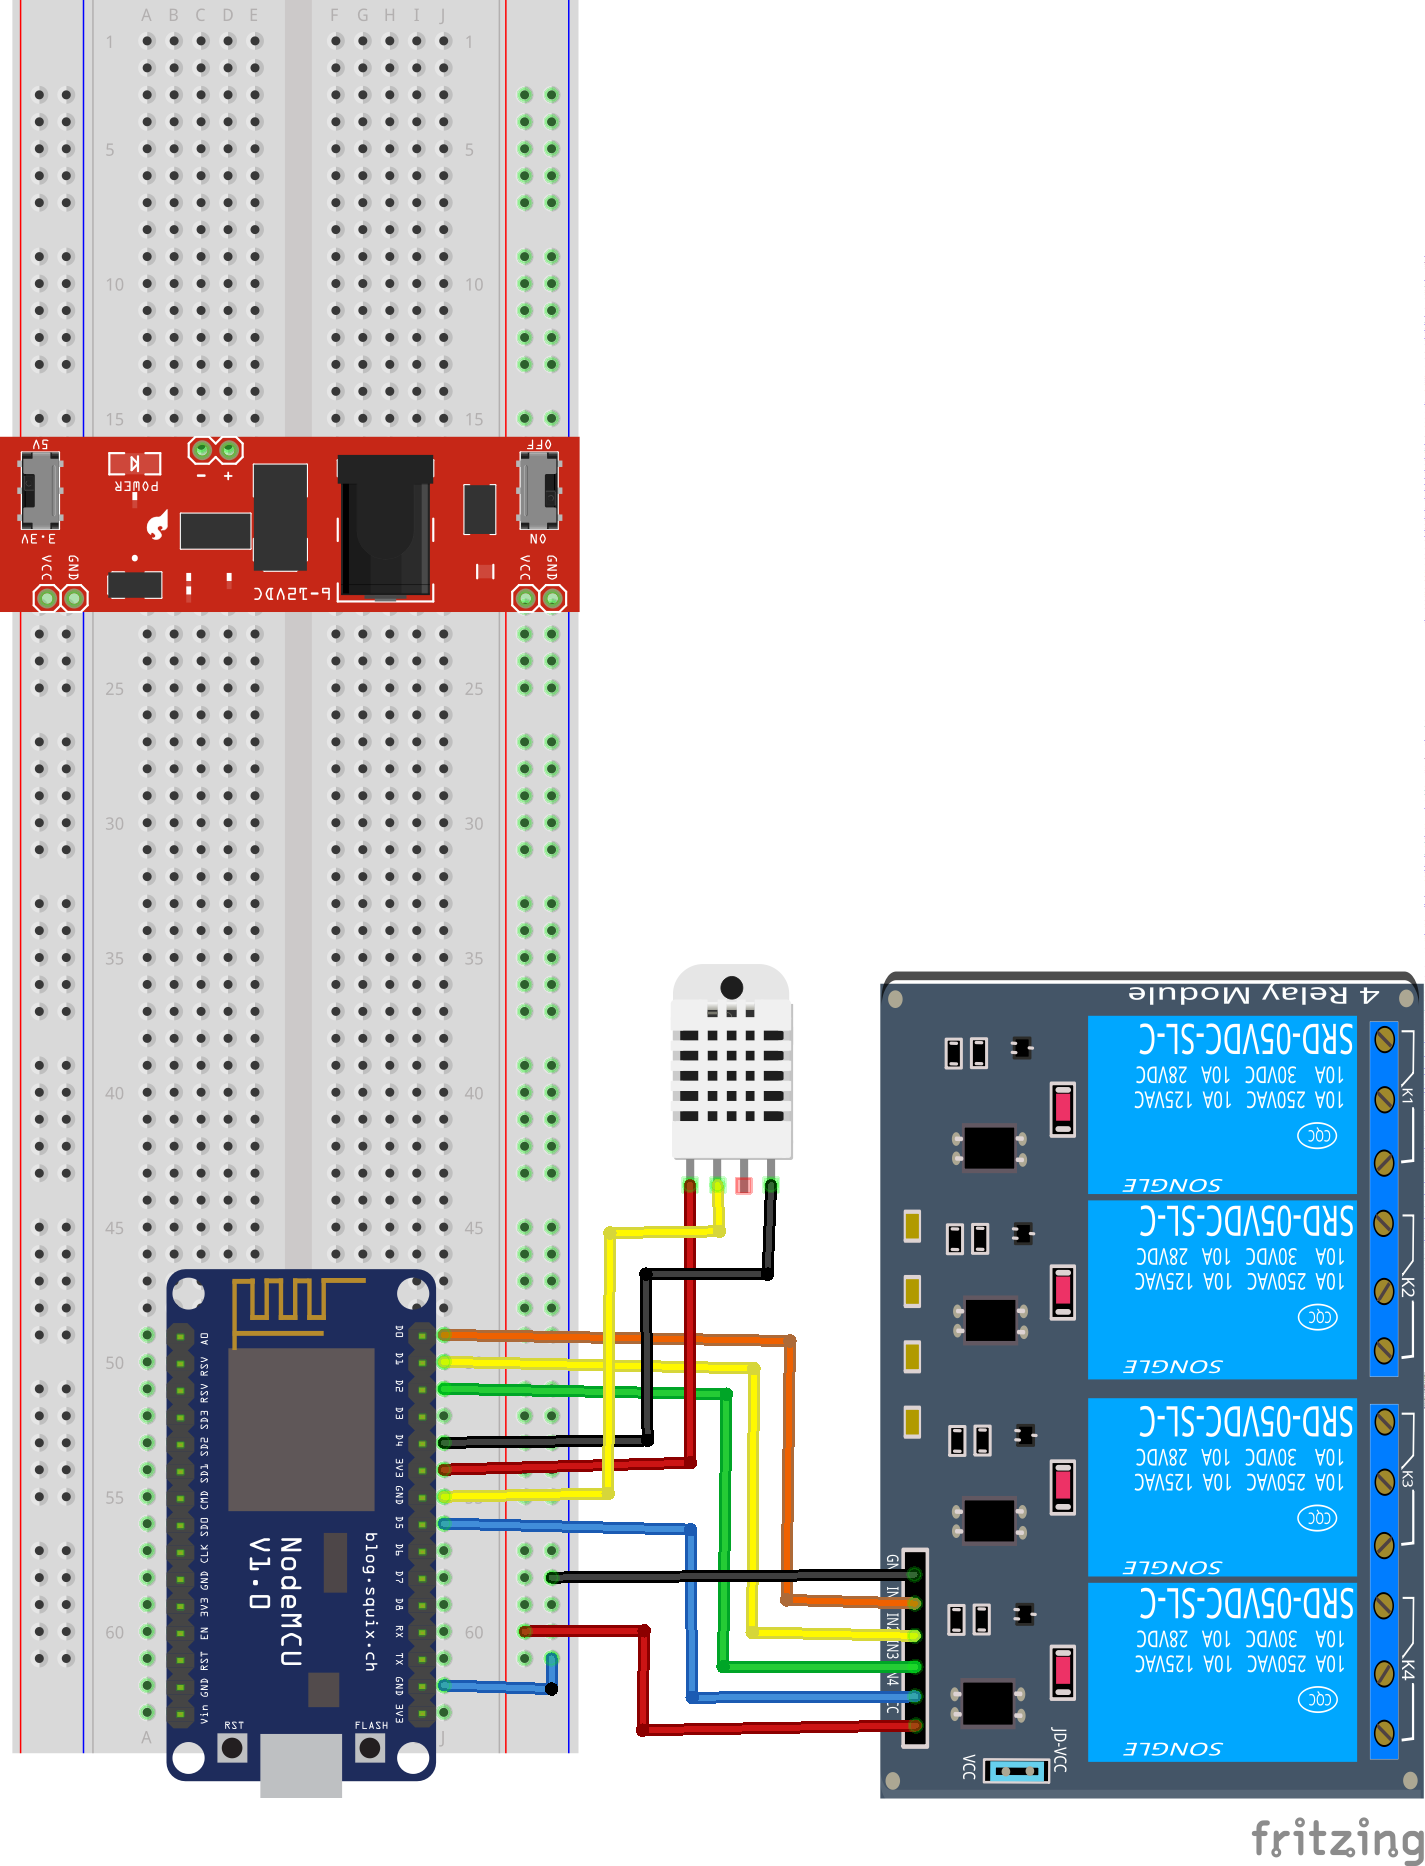
\includegraphics[width=10cm, height=9cm]{Prog10/4.png}
	\caption{Fritizing of Smart Switch Box With NodeMCU and 4-Channel Relay Board}
\end{figure}
\vspace{5mm}

\justify{\textbf{Hooking Up the Circuit}}
\begin{table}[h!]
\centering
\caption{NodeMCU – Relay circuit}
\label{my-label}
\begin{tabular}{|c|c|}
\hline
\textbf{NodeMCU} & \textbf{Relay Pin} \\ \hline
D0 & IN1 \\ \hline
D1 & IN2 \\ \hline
D2 & IN3 \\ \hline
D5 & IN4 \\ \hline
\end{tabular}
\end{table}

\begin{table}[h!]
\centering
\caption{NodeMCU to Power Supply}
\label{my-label}
\begin{tabular}{|c|c|}
\hline
\textbf{NodeMCU} & \textbf{Power Supply} \\ \hline
VCC & 5V \\ \hline
GND & GND \\ \hline
\end{tabular}
\end{table}

\begin{table}[h!]
\centering
\caption{NodeMCU to DHT11}
\begin{tabular}{|c|c|}
\hline
\textbf{NodeMCU} & \begin{tabular}[c]{@{}c@{}}\textbf{Temperature \& Humidity Pin}\end{tabular} \\ \hline
3.3V & VCC \\ \hline
GND & GND \\ \hline
D4 & DATA \\ \hline
\end{tabular}
\end{table}


\justify{\textbf{Step 3: NodeMCU configuration - using Arduino IDE  [Flashing NodeMCU]}\\
Connect the NodeMCU to the computer through a USB cable and invoke arduino IDE   and setup the following to flash the program on to NodeMCU.\\
}
\textbf{File -> Preferences -> Additional Board Manager URLs}
\begin{lstlisting}
  http://arduino.esp8266.com/stable/package_esp8266com_index.json
\end{lstlisting}
\textbf{Tools -> Board Manager-> ESP8266 by ESP8266 Community [Version 2.3.0] \\ Install}

\begin{figure}[h!]
    \centering
	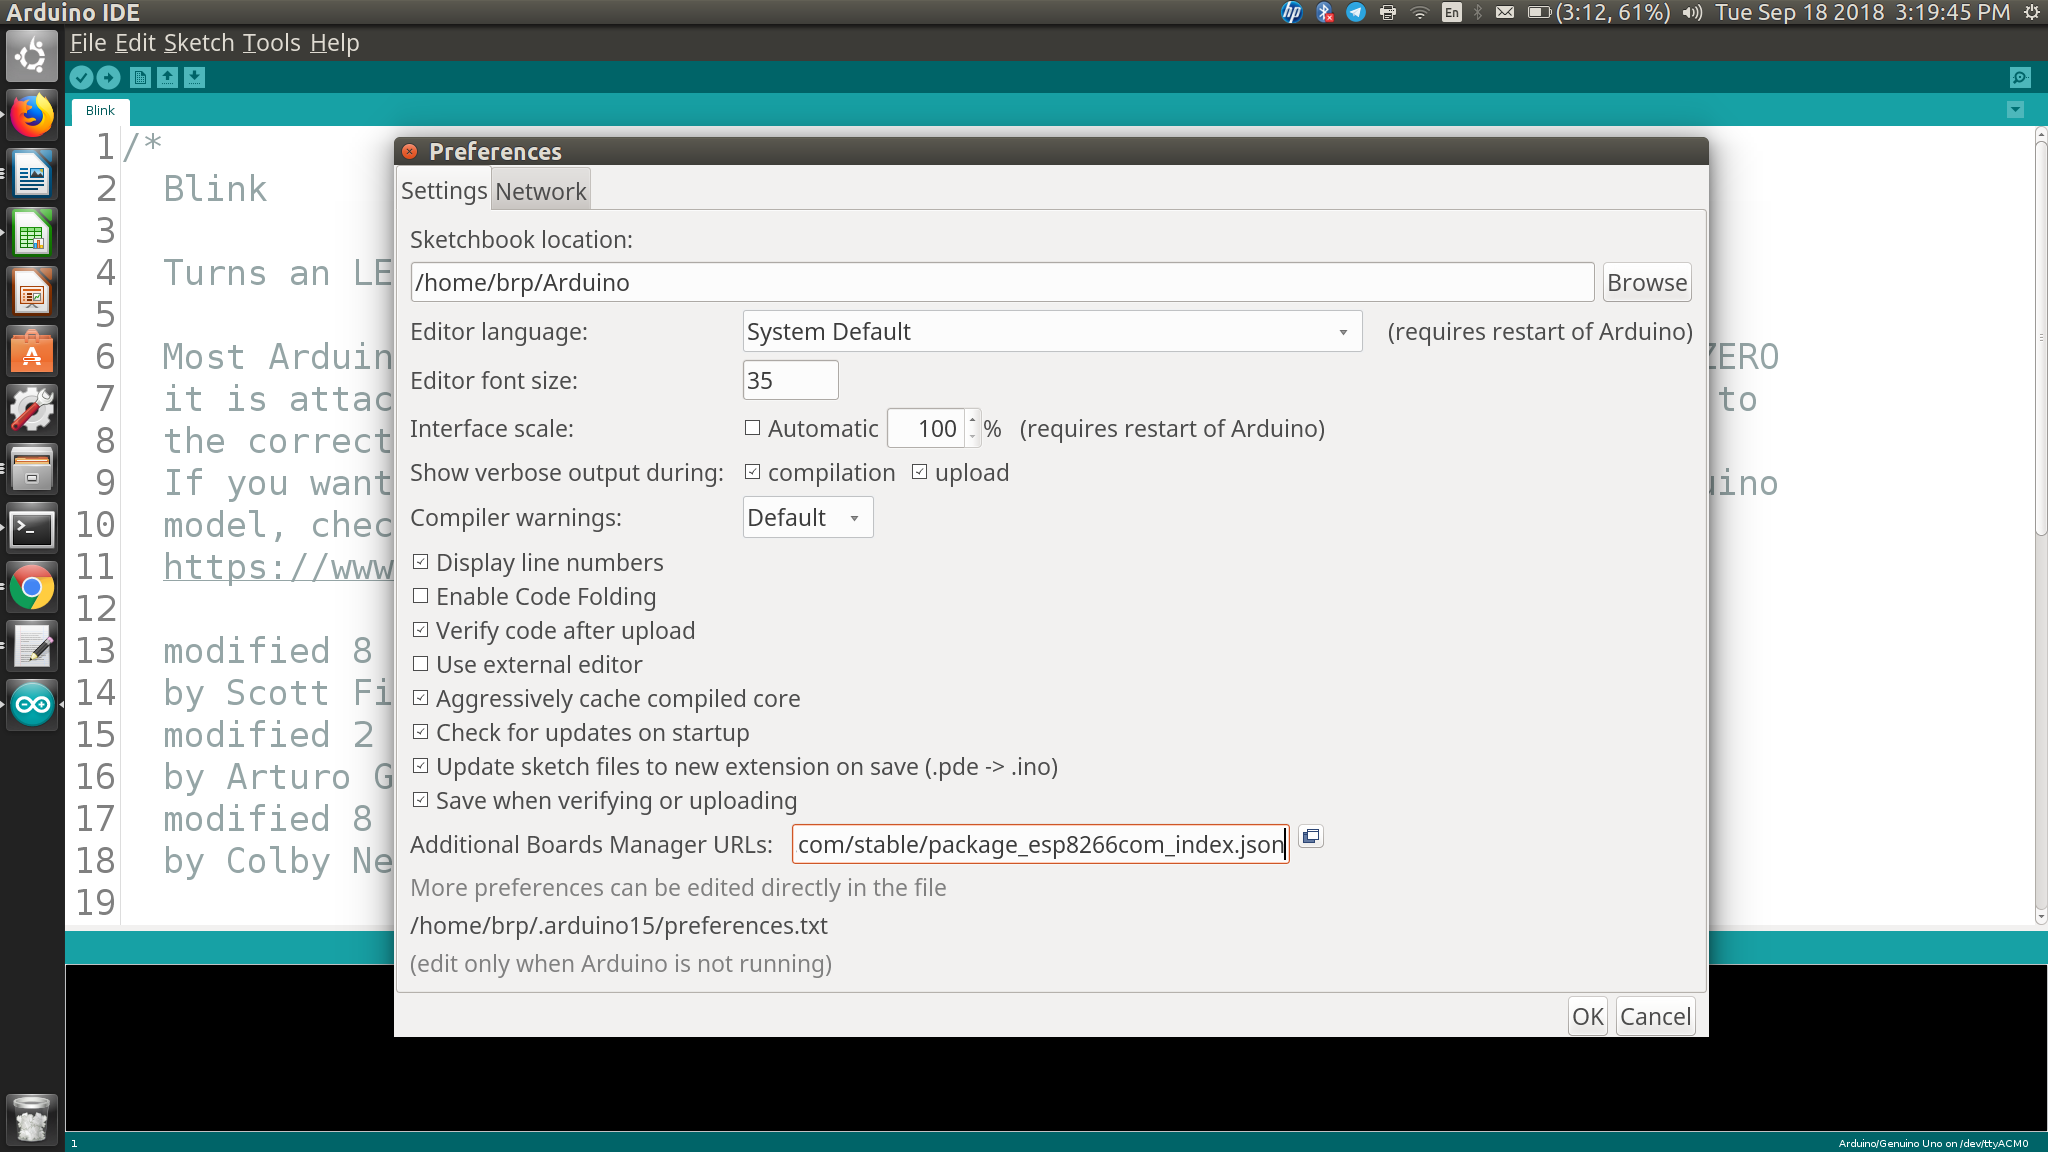
\includegraphics[width=12cm, height=8cm]{Prog10/6.png}
	\caption{Setting Additional Board Manager - Preferences}
\end{figure}
\vspace{5mm}

\justify{\textbf{Selecting and Installation of NodeMCU module i\\
Tools -> Board -> Board manager -> Filter (ESP8266 Community Version) and Install}}

\begin{figure}[h!]
    \centering
	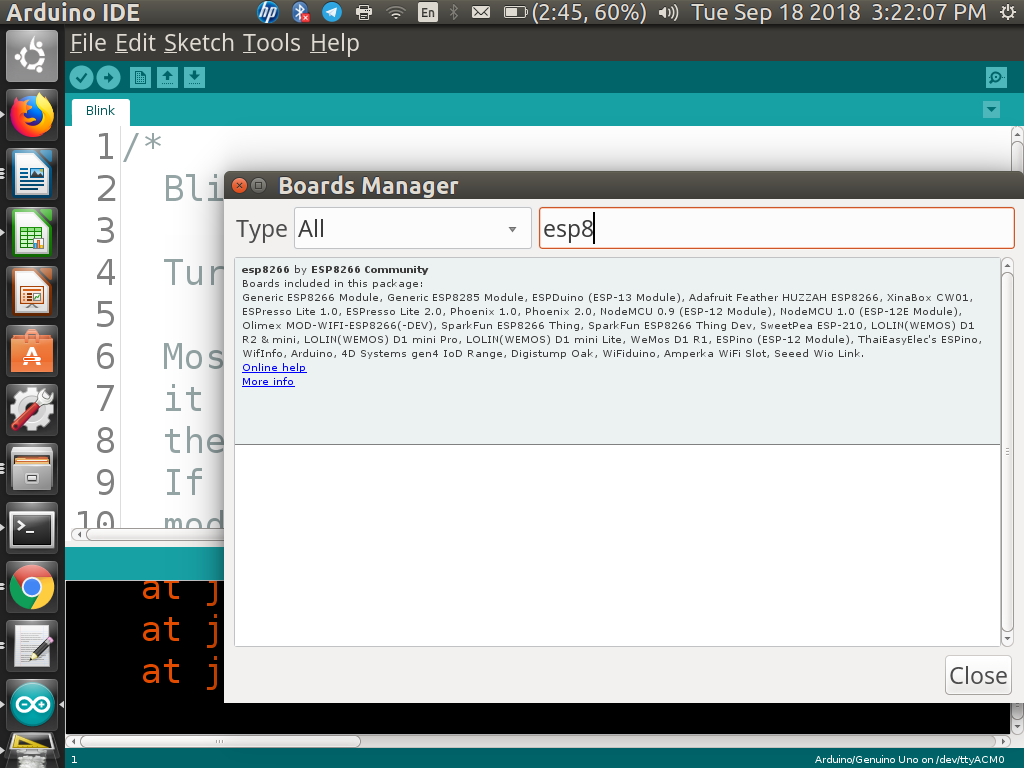
\includegraphics[width=12cm, height=8cm]{Prog10/7.png}
	\caption{Selecting the Board NodeMCU with NodeMCU 1.0(esp 12E module)}
\end{figure}
\vspace{5mm}

\justify{\textbf{Adding libraries for Adafruit MQTT [0.17] and DHT11 \\
Sketch -> Include Libraries-> Manage libraries Adding Adafruit MQTT}}

\begin{figure}[h!]
    \centering
	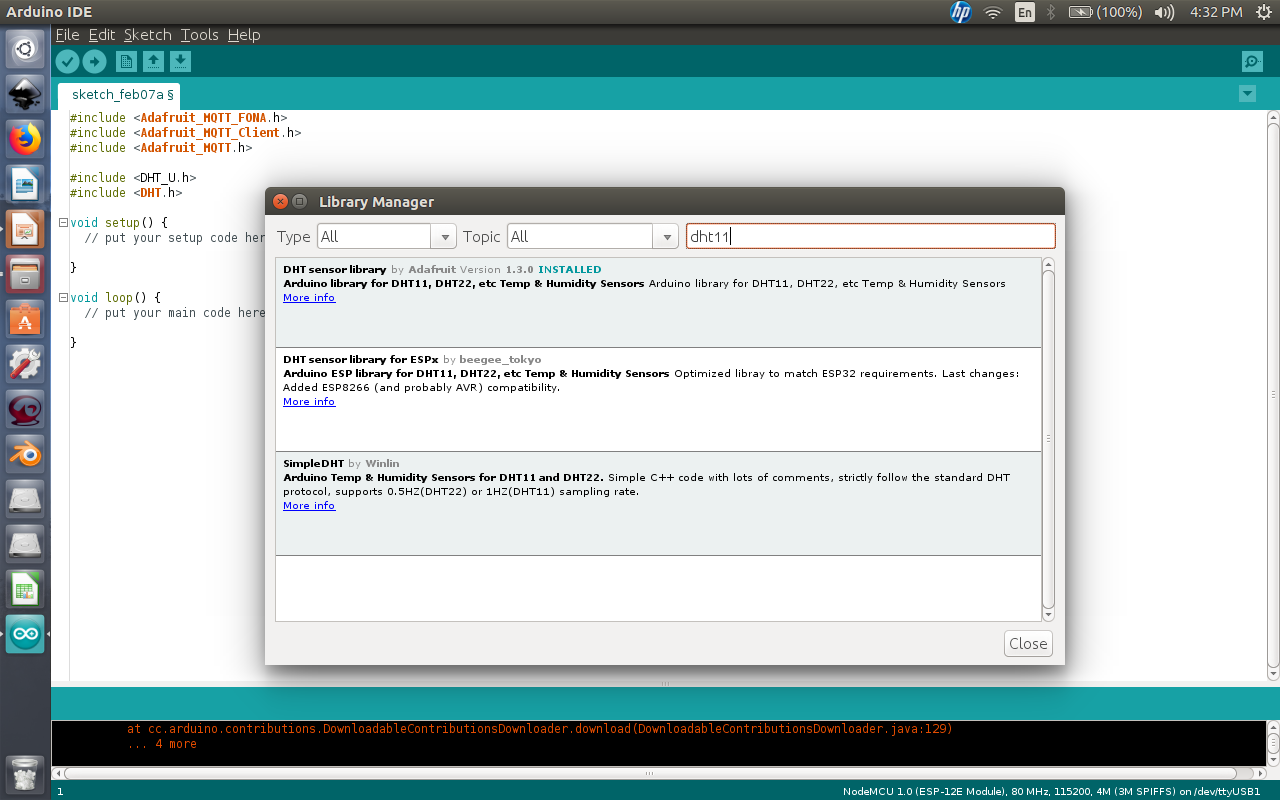
\includegraphics[width=12cm, height=8cm]{Prog10/10.png}
	\caption{Installation of Adafruit MQTT Library Version 0.17}
\end{figure}
\vspace{5mm}
\begin{itemize}[noitemsep,nolistsep]
    \item Load the program on to the IDE
    \item File  ->  Open -> file.ino
    \item Verify / Compile the code [Ctrl+R]
    \item Sketch -> Verify -> Verify/Compile 
    \item Upload if no errors [Ctrl+U]
    \item Sketch -> Upload
\end{itemize}

\begin{lstlisting}[h!]

// including header files for ESP8266, Adafruit and DHT11

#include <ESP8266WiFi.h>
#include "Adafruit_MQTT.h"
#include "Adafruit_MQTT_Client.h"
#include "DHT.h"

// Wi-Fi Access Point

#define WLAN_SSID       "   "   // ssid of your internet connection
#define WLAN_PASS       "   " // password of your ssid
Adafruit.io Setup
#define AIO_SERVER      "io.adafruit.com"
#define AIO_SERVERPORT  1883          // use 8883 for SSL
#define AIO_USERNAME    "   "  // username of io.adafruit.com account
#define AIO_KEY         "  " // key of your user account on adafruit.com


// Feeds / block  Setup a feed called 'onoff' for subscribing to changes.
// this section enables the map the feed created on the dashboard with the program variables
// Note: the feed name is case sensitive 

Adafruit_MQTT_Subscribe Relay = Adafruit_MQTT_Subscribe(&mqtt, AIO_USERNAME "/feeds/FAN");

Adafruit_MQTT_Subscribe Radio = Adafruit_MQTT_Subscribe(&mqtt, AIO_USERNAME "/feeds/LIGHT");
Adafruit_MQTT_Subscribe Charger = Adafruit_MQTT_Subscribe(&mqtt, AIO_USERNAME "/feeds/charger");

Adafruit_MQTT_Subscribe Tv = Adafruit_MQTT_Subscribe(&mqtt, AIO_USERNAME "/feeds/tv");

Adafruit_MQTT_Publish TempandHumid = Adafruit_MQTT_Publish(&mqtt, AIO_USERNAME "/feeds/temperaturehumi");

\end{lstlisting}

\justify{\textbf{Step 4: Dashboard Setup}\\
Signup at https://io.adafruit.com/ \\
Login} \\
Create  a new dash board with the following blocks/feeds with block type as following \\
\begin{table}[]
\centering
\caption{Adafruit Dashboard}
\begin{tabular}{|c|c|}
\hline
\textbf{Block} & \textbf{Block Type} \\ \hline
Light & Toggle \\ \hline
TV & Toggle \\ \hline
Fan & Toggle \\ \hline
Charger & Toggle \\ \hline
Temperature Humidity & Stream \\ \hline
\end{tabular}
\end{table}
\justify{\textbf{Step 5:} Program parameter setup for NodeMCU configuration with Dashboard}
\begin{figure}[h!]
    \centering
	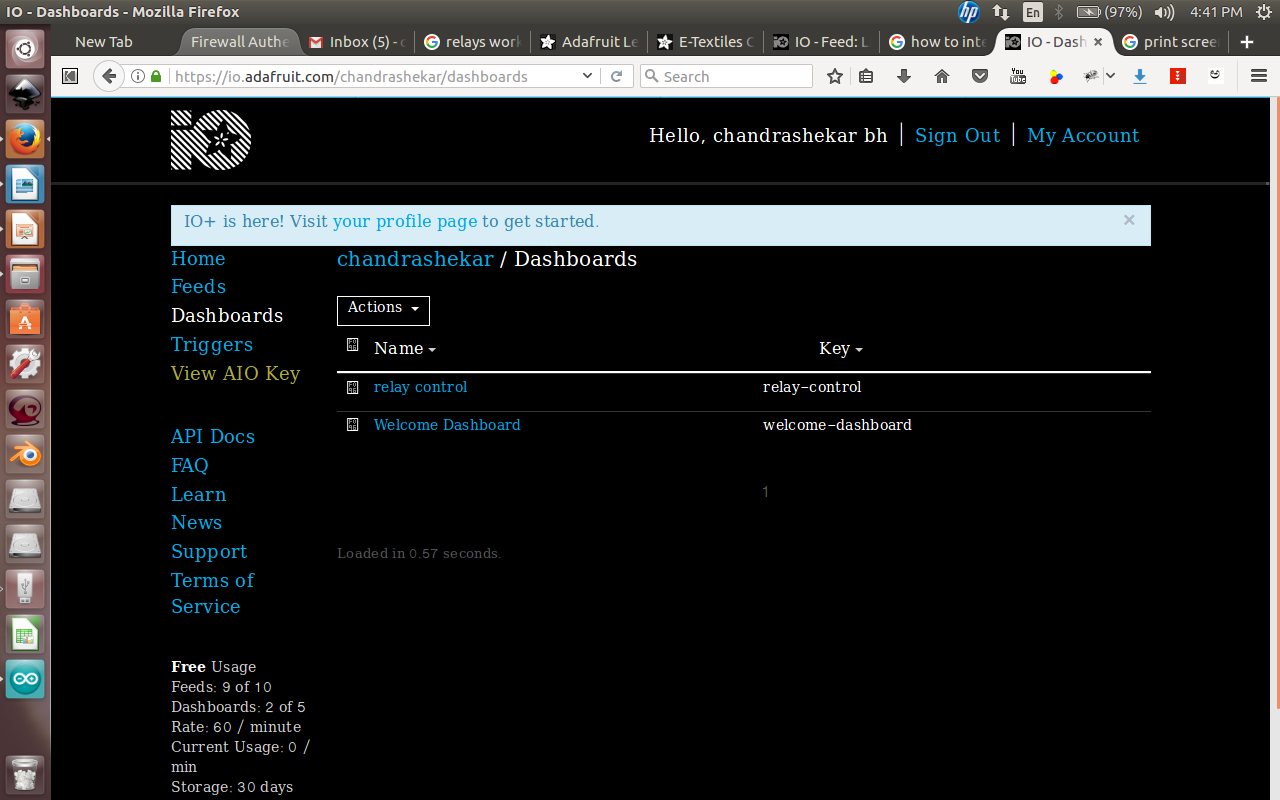
\includegraphics[width=12cm, height=8cm]{Prog10/11.png}
	\caption{Adafruit Dashboard}
\end{figure}
\begin{figure}[h!]
    \centering
	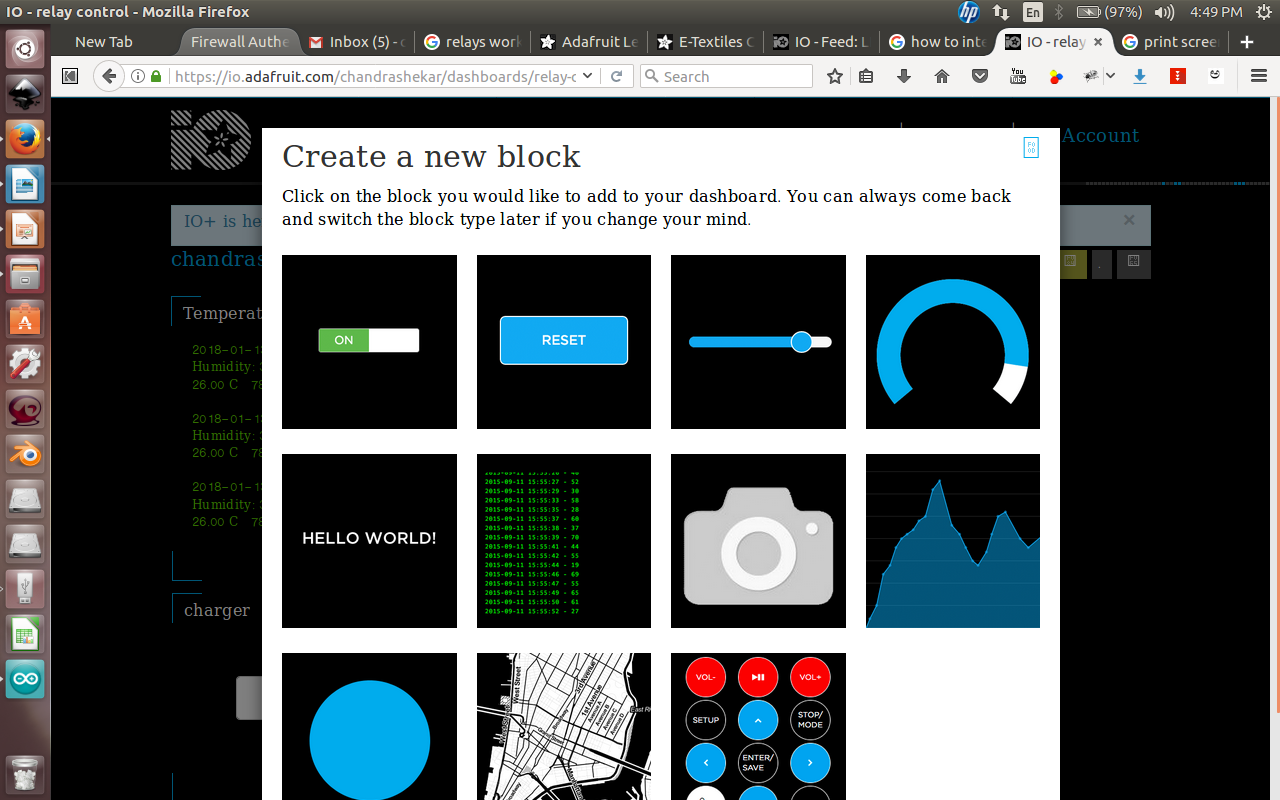
\includegraphics[width=12cm, height=7cm]{Prog10/12.png}
	\caption{Adafruit Dashboard - Home Page}
\end{figure}
\begin{figure}[h!]
    \centering
	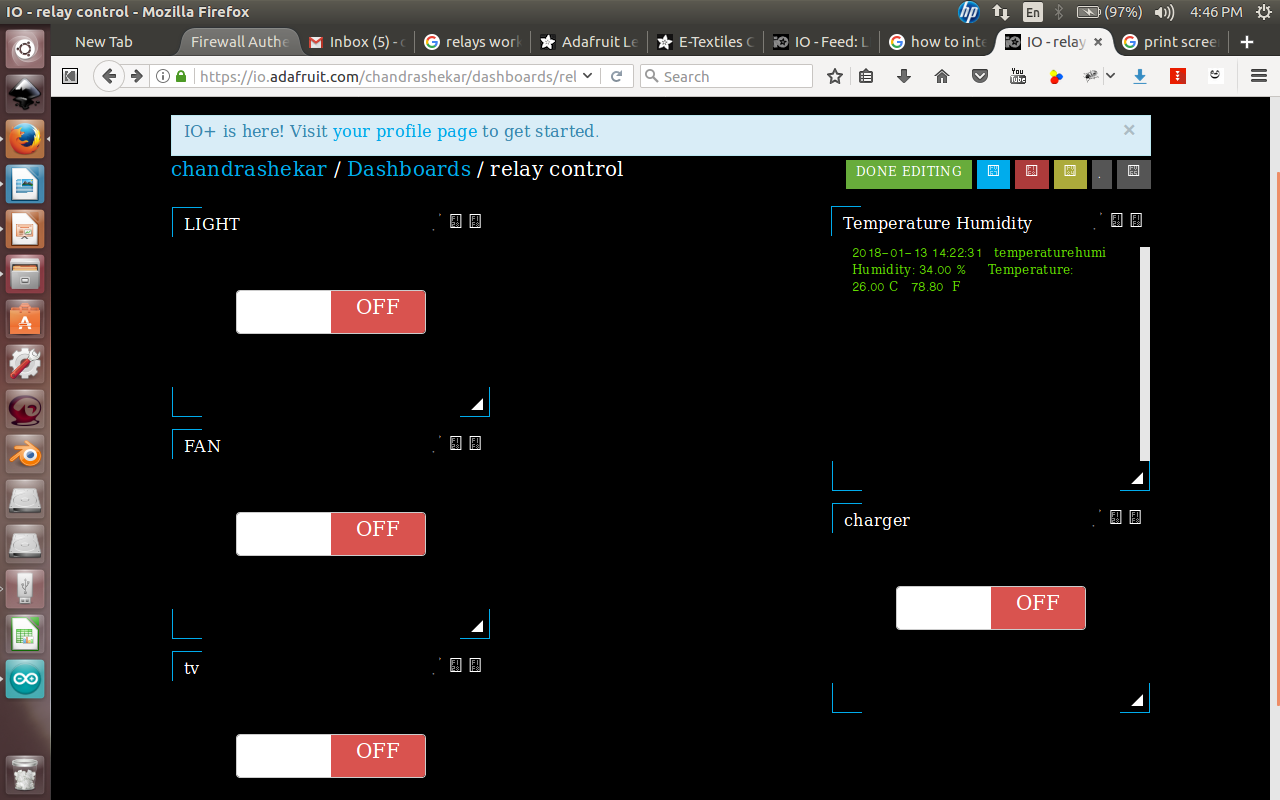
\includegraphics[width=12cm, height=7cm]{Prog10/13.png}
	\caption{Creating a New Block/Feed in Adafruit Dashboard}
\end{figure}
\justify{\textbf{Step 6: Execution}\\
\begin{itemize}
    \item Compile and upload the program from arduino IDE to NodeMCU
    \item Ensure the Internet connection parameters are satisfied for NodeMCU to hook on to the Dashboard Website
    \item Use the URL of the dashboard www.io.Adafruit.com to load the dashboard and operate on the feeds created.
\end{itemize}
}
\end{flushleft}\vspace{6.5cm}

\begin{table}[!b]
\centering
\begin{tabular}{| >{\centering\arraybackslash}m{0.5in}| >{\arraybackslash}m{3.5in}| >{\centering\arraybackslash}m{0.8in}| >{\centering\arraybackslash}m{0.9in}|}
\hline \hline
& & &\\
\textbf{S.No}  & \hspace{1.7cm}\textbf{Rubrics for Practice Sessions} & \textbf{Max Marks} & \textbf{Marks Obtained} \\
& & &\\ \hline
1 & Physical design of circuits with devices & 2 &\\ \hline
2 & Development of Sketch/Script & 1 &\\ \hline
3 & Results & 2 &\\ \hline
4 & Clarity about the method/procedure adoption & 2 &\\ \hline
5 & Diagrams depicting connections between development boards, breadboards \& devices with Viva Voce & 3 &\\\hline
\multicolumn{2}{|c|}{} &  &\\
\multicolumn{2}{|c|}{\raggedright \textbf{\large{Total}} } & 10 &\\\hline
\multicolumn{2}{|c|}{} &  \multicolumn{2}{c|}{}\\
\multicolumn{2}{|c|}{\raggedright \textbf{\large{Signature of Faculty}} } &  \multicolumn{2}{c|}{}\\
\hline\hline
\end{tabular}
\end{table}

\clearpage
\center \textbf{Program No. 6}\vspace{11cm}

Paste your DATA SHEET here\\
\textit{[Page intentionally left blank, student to paste his/her data sheet after evaluated by the faculty in-charge] }
\clearpage
%--------------------------------------------------------------------------------------------------------------------------------------
\begin{center}
{\large \textbf{Part B}\\  {\textbf{Program - 7}}\\
Integrate Blynk / ThingsBoard to any of the experiments done above
or
any Sensor / Actuator used in the experiments above (PART A).}
\end{center}
\begin{flushleft}
\textbf{\textit{Components Required}}
\begin{itemize}[noitemsep,nolistsep]
\item 1 x NodeMCU
\item 1 x Relay Switch
\item 1 x DHT11
\end{itemize}
\vspace{5mm}

\textbf{\textit{Library Files}}\\ 
Install DHT Library File Version 1.2.3 and Blynk Library File Version 0.5.3 using Library Manager and include in the Program
\vspace{4mm}

\textbf{Step 1:} Set the SSID Name and Password\\
\vspace{4mm}

\textbf{Step 2:} Set Port and Board
\vspace{4mm}

\textbf{Step 3:} Download Blynk Application from Store and Login
\vspace{4mm}

\textbf{Step 4:} Create a Project and Set the Project Name and Select NodeMCU
\vspace{4mm}

\textbf{Step 5:} Add Two Buttons, Add the Gauge ans Assign Labels\\
\vspace{3mm}
\hspace{10mm}  a. First Button to control relay ,assign DIGITAL PIN 0,set MODE to SWITCH \\
\hspace{10mm} b. Second Button to get humidity value and assign VIRTUAL PIN 1\\ \vspace{3mm}
Add a Gauge to Show Temperature, Assign VIRTUAL PIN 0\\
Add Labels to Show Humidity Value, Assign VIRTUAL PIN 2\\
\vspace{4mm}
\textbf{Step 6:} \\
\hspace{10mm} a. Get AUTH key from the Project in Blynk Application and Assign it to a variable in NodeMCU Program \\
\hspace{10mm} b. Add SSID and Password values in NodeMCU Program
\vspace{4mm}

\textbf{\textit{Code}}
\begin{lstlisting}
#include <DHT.h>//version 1.2.3
#include <BlynkSimpleEsp8266.h>//version 0.5.3
#include <ESP8266WiFi.h>
const char* ssid = "ssid";
const char* password = "password";
char auth[] = "your token";
DHT dht(D1, DHT11);//set pin D1 to DHT11
BlynkTimer timer;
void setup()
{
  //  Serial.begin(9600); // Initializing serial port for debugging purposes  
  Blynk.begin(auth, ssid, password);
  timer.setInterval(1000L, gettemp);// Setup a function to be called every second
}
BLYNK_WRITE(V1){ // triggred when V1 is used
  float h = dht.readHumidity();
  Blynk.virtualWrite(V2, h); // return humidity value to V2
  }
void gettemp(){ 
  float t = dht.readTemperature();
  if (!isnan(t)){
    Blynk.virtualWrite(V0,t); // or dht.readTemperature(true) for Fahrenheit   
    }
 }
void loop() {
  // put your main code here, to run repeatedly:
  Blynk.run();
 timer.run();  
}
\end{lstlisting}

\textbf{\textit{Fritzing}} \\
\begin{figure}[h!]
    \centering
	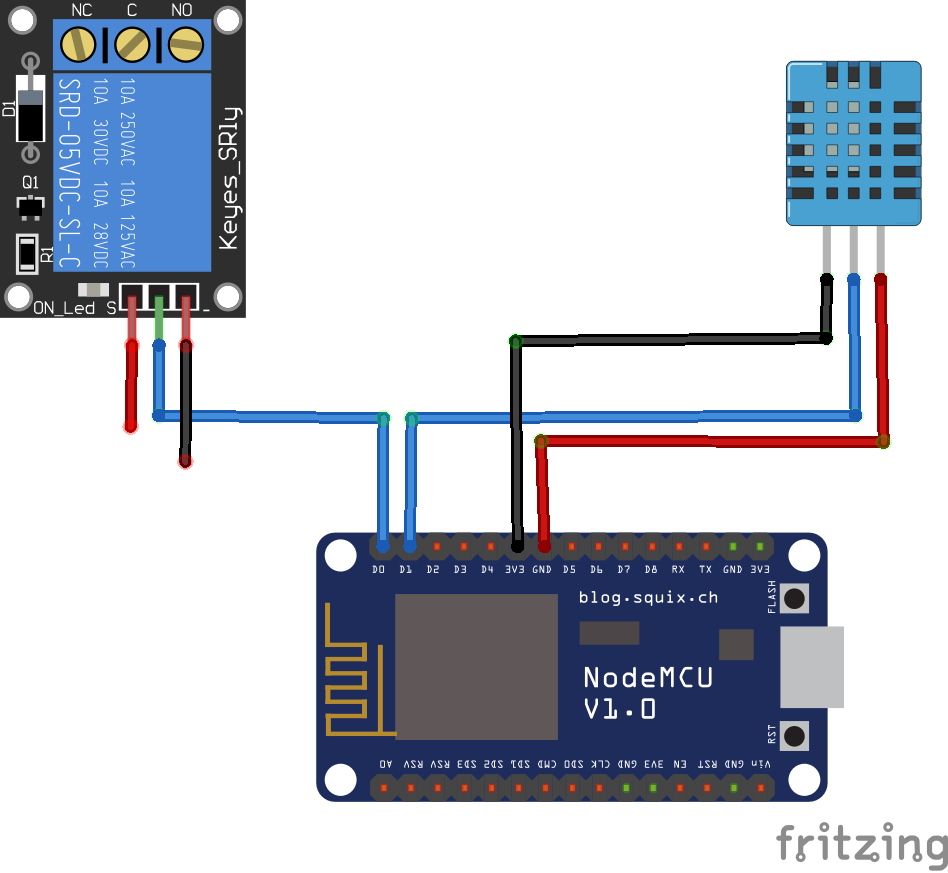
\includegraphics[width=12cm, height=8cm]{Prog7.png}
	\caption{Fritzing for Program 7}
\end{figure}
\end{flushleft}

\begin{figure}[h!]
\centerline{%
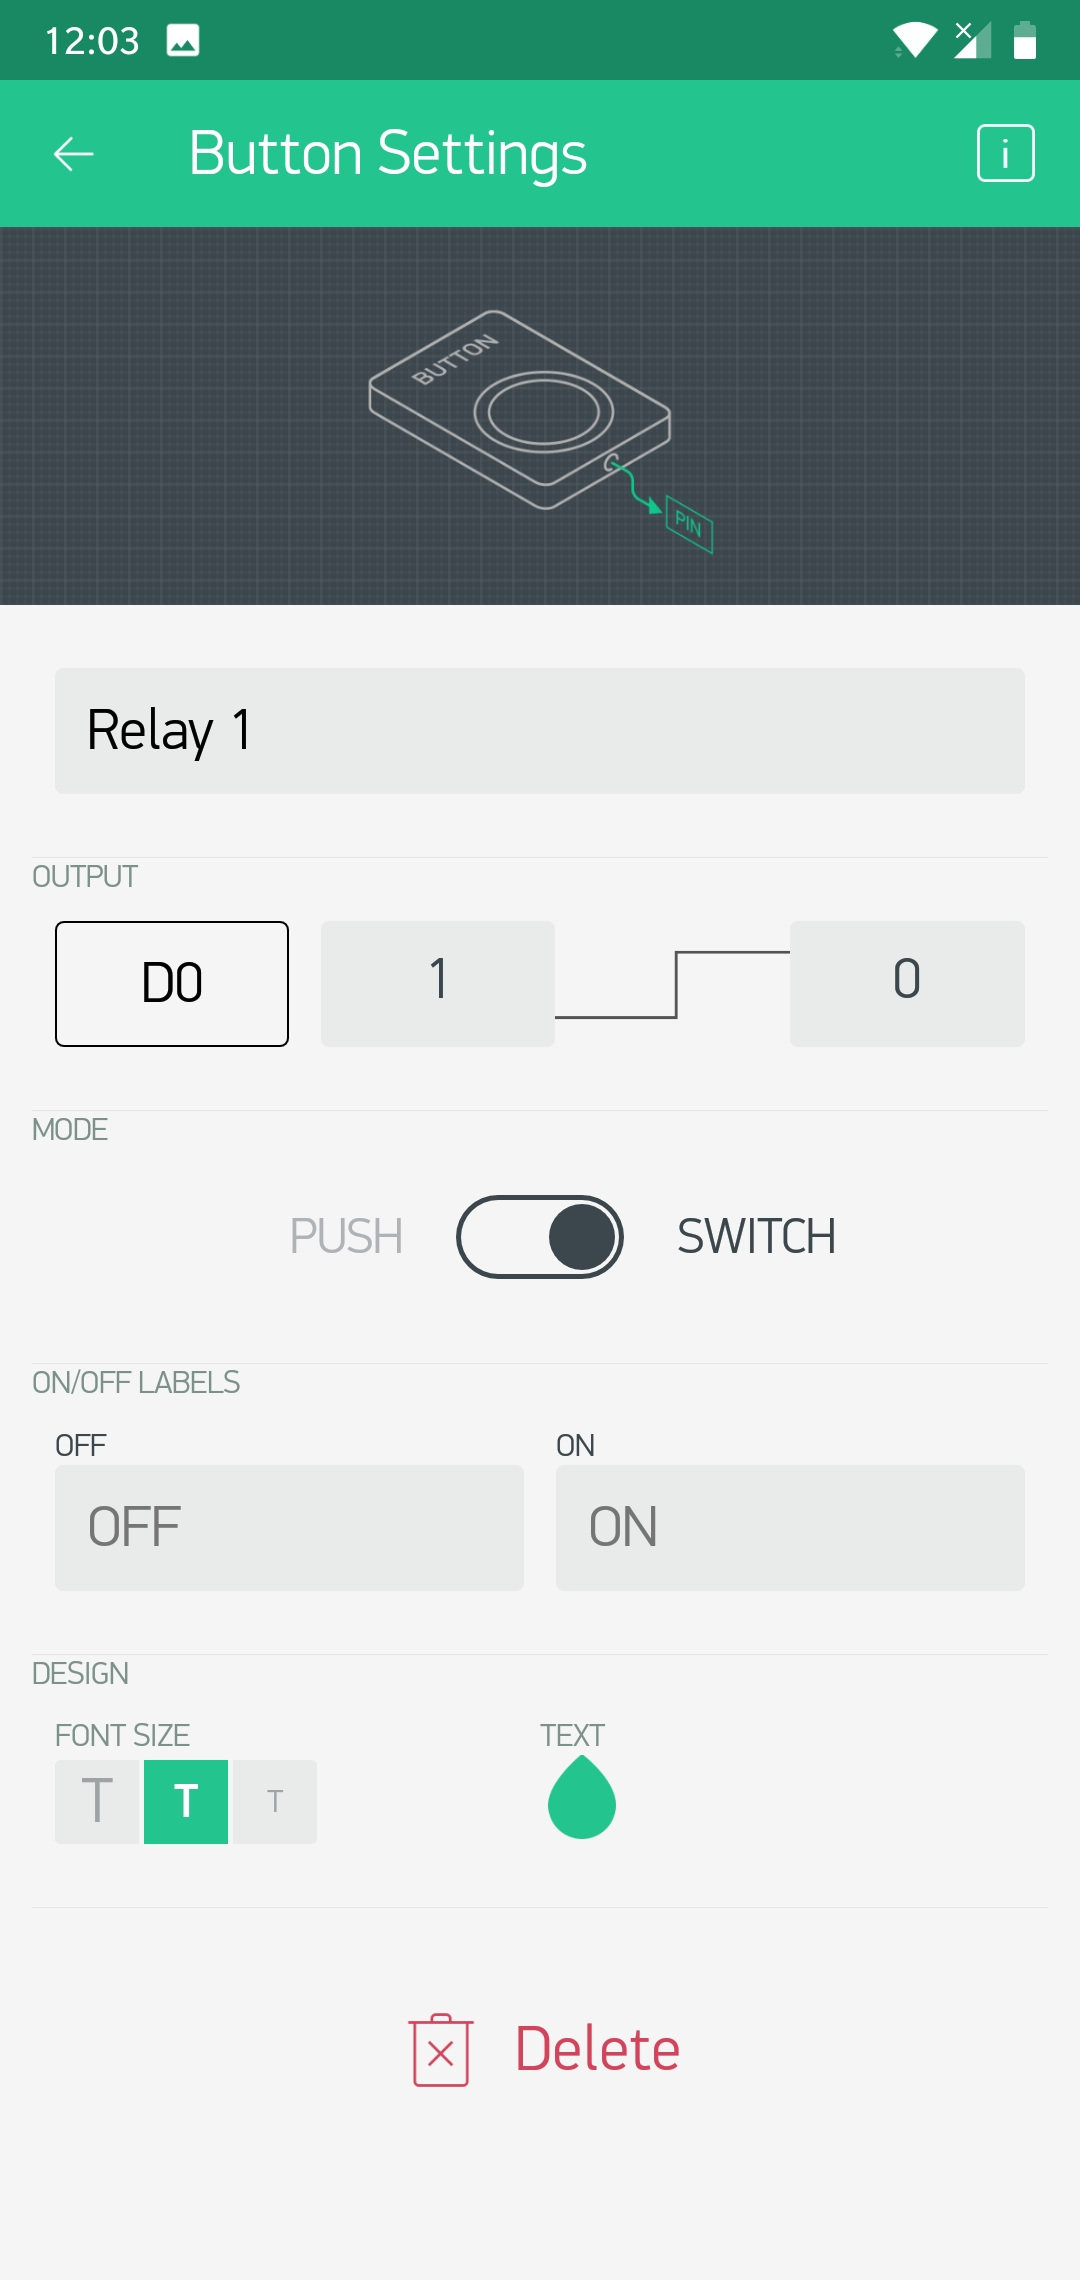
\includegraphics[width=9cm,height=11cm]{Lab7_1.jpg}%
\hspace{0.5 cm}
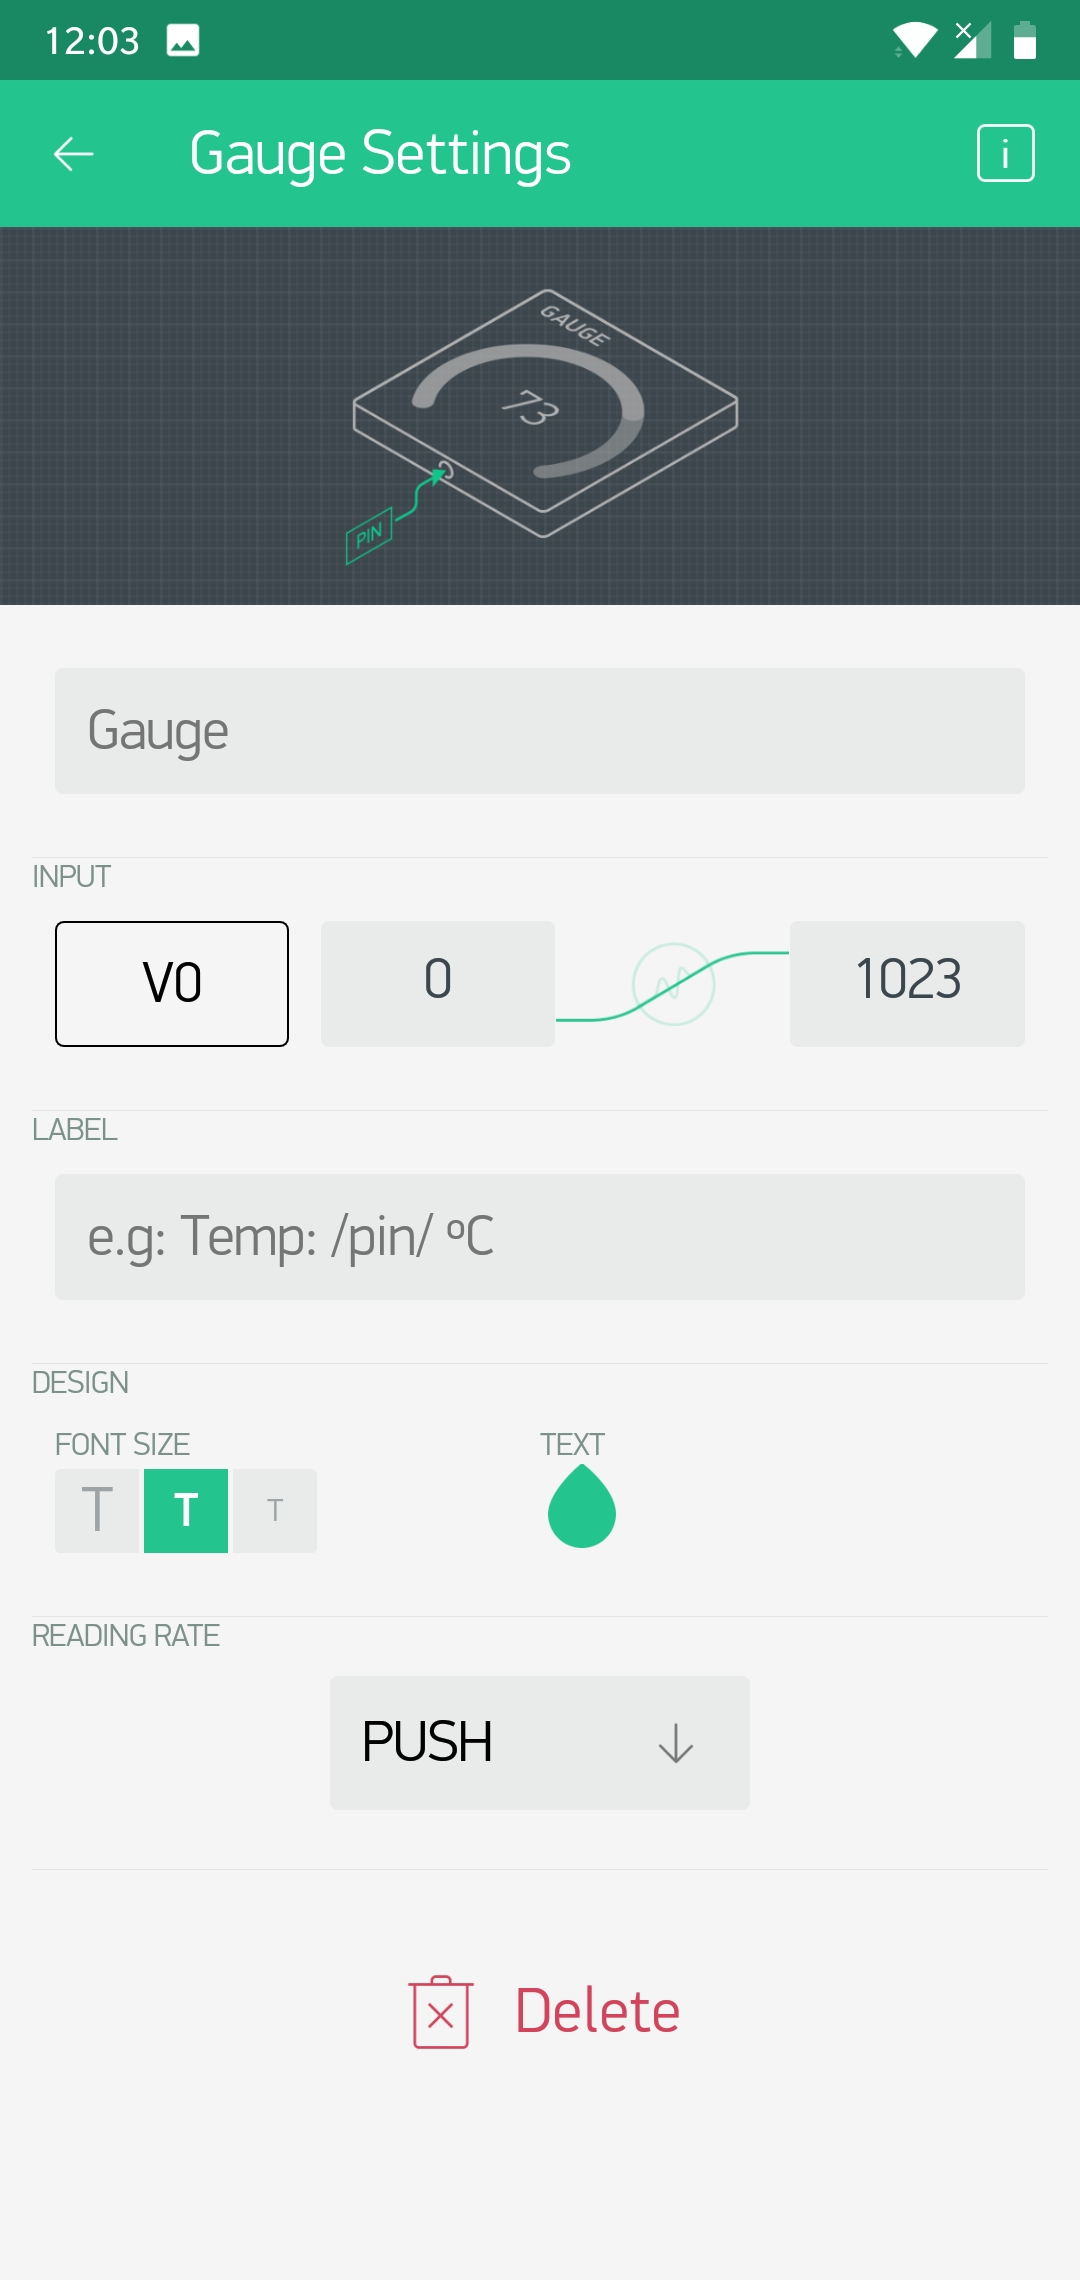
\includegraphics[width=9cm,height=11cm]{Lab7_2.jpg}%}
}
\end{figure}
\begin{figure}[h!]
\centerline{%
\includegraphics[width=9cm,height=11cm]{Lab7_3.jpg}%
\hspace{0.5 cm}
\includegraphics[width=9cm,height=11cm]{Lab7_4.jpg}%}
}
\end{figure}
\begin{table}[!b]
\centering
\begin{tabular}{| >{\centering\arraybackslash}m{0.5in}| >{\arraybackslash}m{3.5in}| >{\centering\arraybackslash}m{0.8in}| >{\centering\arraybackslash}m{0.9in}|}
\hline \hline
& & &\\
\textbf{S.No}  & \hspace{1.7cm}\textbf{Rubrics for Practice Sessions} & \textbf{Max Marks} & \textbf{Marks Obtained} \\
& & &\\ \hline
1 & Physical design of circuits with devices & 2 &\\ \hline
2 & Development of Sketch/Script & 1 &\\ \hline
3 & Results & 2 &\\ \hline
4 & Clarity about the method/procedure adoption & 2 &\\ \hline
5 & Diagrams depicting connections between development boards, breadboards \& devices with Viva Voce & 3 &\\\hline
\multicolumn{2}{|c|}{} &  &\\
\multicolumn{2}{|c|}{\raggedright \textbf{\large{Total}} } & 10 &\\\hline
\multicolumn{2}{|c|}{} &  \multicolumn{2}{c|}{}\\
\multicolumn{2}{|c|}{\raggedright \textbf{\large{Signature of Faculty}} } &  \multicolumn{2}{c|}{}\\
\hline\hline
\end{tabular}
\end{table}


\clearpage
\center \textbf{Program No. 7}\vspace{11cm}

Paste your DATA SHEET here\\
\textit{[Page intentionally left blank, student to paste his/her data sheet after evaluated by the faculty in-charge] }

\clearpage


\begin{center}
{\large {\textbf{Program - 8}}\\
Integrate Adafruit /Thingsboard Dashbaord with Arduino,
Raspberry Pi and any Sensor / Actuator.}\\
\end{center}
\begin{flushleft}
\textbf{Note:} The Dashboard done for Program 7 should not be used. Students deploy any of the dashboard mentioned in the exam
\end{flushleft}
\justify{
\textbf{\textit{Instructions}}\\
\vspace{2mm}
Refer the following link that describes the steps to install Thingsboard dashboard on Raspberry Pi3 Model B -
\url{https://thingsboard.io/docs/user-guide/install/rpi/}
\\
Subsequently the following links helps in 
\begin{itemize}
    \item Getting started with Thingsboard \\
        \url{https://thingsboard.io/docs/guides#AnchorIDGettingStartedGuides}
        \item Installing Thingsboard on operating systems \\
        \url{https://thingsboard.io/docs/guides#AnchorIDInstallationGuides}
        \item Configuring Sensors with Dashboard \\
        \url{https://thingsboard.io/docs/guides#AnchorIDConnectYourDevice}
        \item An example to configure DHT22 with Thingsboard can be referred from the link below \\ \url{https://thingsboard.io/docs/samples/raspberry/temperature/}
\end{itemize}
}
\begin{table}[!b]
\centering
\begin{tabular}{| >{\centering\arraybackslash}m{0.5in}| >{\arraybackslash}m{3.5in}| >{\centering\arraybackslash}m{0.8in}| >{\centering\arraybackslash}m{0.9in}|}
\hline \hline
& & &\\
\textbf{S.No}  & \hspace{1.7cm}\textbf{Rubrics for Practice Sessions} & \textbf{Max Marks} & \textbf{Marks Obtained} \\
& & &\\ \hline
1 & Physical design of circuits with devices & 2 &\\ \hline
2 & Development of Sketch/Script & 1 &\\ \hline
3 & Results & 2 &\\ \hline
4 & Clarity about the method/procedure adoption & 2 &\\ \hline
5 & Diagrams depicting connections between development boards, breadboards \& devices with Viva Voce & 3 &\\\hline
\multicolumn{2}{|c|}{} &  &\\
\multicolumn{2}{|c|}{\raggedright \textbf{\large{Total}} } & 10 &\\\hline
\multicolumn{2}{|c|}{} &  \multicolumn{2}{c|}{}\\
\multicolumn{2}{|c|}{\raggedright \textbf{\large{Signature of Faculty}} } &  \multicolumn{2}{c|}{}\\
\hline\hline
\end{tabular}
\end{table}


\clearpage
\center \textbf{Program No. 8}\vspace{11cm}

Paste your DATA SHEET here\\
\textit{[Page intentionally left blank, student to paste his/her data sheet after evaluated by the faculty in-charge] }

\clearpage
%----------------------------------------------------------------------------------------------------
%--------------------------------------------------------------------------------------------------------------------------------------
\begin{center}
{\large{\textbf{Program - 9}}\\
Develop a django dashboard to monitor and control the sensor and actuators used in PART A}
\end{center}
\begin{flushleft}
\textbf{\textit{Components Required}}
\begin{itemize}[noitemsep,nolistsep]
\item DHT11 Data Pin-GPIO 04(Pin 07)
\end{itemize}
\vspace{5mm}

\textbf{Step 1:} Download and install the software and libraries from the following links \\
\vspace{5mm}

\textbf{\textit{Library Files}}\\ \begin{itemize}[noitemsep,nolistsep]
\item sudo pip install django or sudo pip install django==1.11.14
\item sudo git clone https://github.com/adafruit/Adafruit\_Python\_GPIO.git
\item sudo git clone https://github.com/adafruit/Adafruit\_Python\_SSD1306.git
\item sudo git clone https://github.com/adafruit/Adafruit\_Python\_DHT.git
\end{itemize}
\vspace{5mm}

\textbf{Step 2:} Connect the components as specified below\\
Note: Refer the Fritzing for more information on connecting the components
\vspace{5mm}

\textbf{OLED}
\begin{itemize}[noitemsep,nolistsep]
\item SCK - GPIO 11(PIN 23)
\item SDA - GPIO 10(PIN 19)
\item RES - GPIO 25(PIN 22)
\item DC - GPIO 24(PIN 18)
\item CS - GPIO 08(PIN 24)
\end{itemize}

\textbf{LED}
\begin{itemize}
    \item LED Positive Pin - GPIO 14 (PIN 8) 
\end{itemize}

\textbf{\textit{Code}}\\

\textbf{Step 3:}
Install the Adafruit Python GPIO Library
\begin{lstlisting}
cd ~
sudo git clone https://github.com/adafruit/Adafruit_Python_GPIO.git
cd Adafruit_Python_GPIO
sudo python setup.py install
\end{lstlisting}
\vspace{5mm}
\textbf{Step 4:}
Install the SSD1306 Python library (OLED)

\begin{lstlisting}
cd ~
sudo git clone https://github.com/adafruit/Adafruit_Python_SSD1306.git
cd Adafruit_Python_SSD1306
sudo python setup.py install
\end{lstlisting}
\clearpage

\textbf{Step 5:}
To Enable SPI
\begin{lstlisting}
sudo raspi-config
\end{lstlisting}
\vspace{5mm}
\textbf{Step 6:} Install the DHT11 python library

\begin{lstlisting}
cd ~
sudo git clone https://github.com/adafruit/Adafruit_Python_DHT.git
cd Adafruit_Python_DHT
sudo python setup.py install
\end{lstlisting}
\vspace{5mm}

\textbf{Step 7:} Install Django
\begin{lstlisting}
cd ~ 
sudo pip install django or sudo pip install django==1.11.14
\end{lstlisting}
\vspace{5mm}
Note: If pip is broken
\begin{lstlisting}
curl https://bootstrap.pypa.io/get-pip.py -o get-pip.py
sudo python get-pip.py --force-reinstall
\end{lstlisting}
\vspace{5mm}

\textbf{Step 8:} Create Directory and Setting Permission
\begin{lstlisting}
create directory && chmod 777 <directory name>
sudo django-admin.py startproject lab9
cd lab9
sudo python manage.py migrate
\end{lstlisting}
\vspace{5mm}

\textbf{Step 9:} To host Server using Raspberry Pi IP Address
\begin{lstlisting}
cd lab9
sudo nano settings.py
#search for ALLOW HOST and ADD IP ADDRESS of Raspberry Pi
ALLOWED_HOSTS = ['192.168.0.104']
\end{lstlisting}
\vspace{5mm}

\textbf{Step 10:} To check if server starts without error
\begin{lstlisting}
cd ..
sudo python manage.py runserver <Raspberry pi IP:PORT>
#exit from server
Ctrl+c
\end{lstlisting}
\vspace{5mm}

\textbf{Step 11:} Create Templates Folder to store HTML Files
\begin{lstlisting}
sudo mkdir templates
cd lab9
\end{lstlisting}
\vspace{5mm}

\textbf{Step 12:} Create views.py file \\
\vspace{5mm}
\textbf{Step 13:} In views.py, Create a definition to return index.html page and Class from LED, OLED \\
\vspace{5mm}
\textbf{Step 14:} Coding - utf-8 \\
\begin{lstlisting}
from __future__ import unicode_literals
from django.shortcuts import render
from django.views.generic import View,TemplateView
import Adafruit_DHT
import RPi.GPIO as GPIO
from django.http import HttpResponseRedirect
import sys
import time
import Adafruit_GPIO.SPI as SPI
import Adafruit_SSD1306
from PIL import Image
from PIL import ImageDraw
from PIL import ImageFont
import subprocess
\vspace{5mm}
\textbf{Step 15:}Create views here
\begin{lstlisting}
def homepage(request):#render index.html
        humid, temp = Adafruit_DHT.read_retry(11, 4)
        return render(request,'index.html',{"tempdata":temp,"humiddata":humid})#send temperature and humididty data
class led(View):#led ON and OFF
        def post(self,request):
                GPIO.setmode(GPIO.BCM)
                GPIO.setup(14,GPIO.OUT)#PIN NO 14
                if(GPIO.input(14)):#check if pin is in HIGH status
                        print("on->off")
                        GPIO.output(14,False)
                else:
                     print("off->on")
                        GPIO.output(14,True)
                return HttpResponseRedirect("/")#redirect to index.html page

class oled(View):#oled 
        def post(self,request):
                lines=[request.POST.get('oleddata')]#get form data from post request
                disp = Adafruit_SSD1306.SSD1306_128_64(rst=25, dc=24, sclk=11, din=10, cs=8)#7pin oled
                disp.begin()
                disp.clear()
                disp.display()
                width = disp.width
                height = disp.height
                image = Image.new('1', (width, height))
                draw = ImageDraw.Draw(image)
                draw.rectangle((0,0,width,height), outline=0, fill=0)
                padding = -2
                top = padding
                bottom = height-padding
                x = 0
                font = ImageFont.load_default()
                draw.rectangle((0,0,width,height), outline=0, fill=0)
                extra1 = 0
                extra2 = 0
                for i in range(0,len(lines)):
                        draw.text((x+extra1,top+extra2),str(lines[i]),font=font,fill=255)
                        #extra1+=15
                        extra2 += 8
                disp.image(image)
                disp.display()
                return HttpResponseRedirect("/")
                #redirect to index.html page
\end{lstlisting}
\vspace{5mm}
\textbf{Step 16:} Add the url pattern to render index.html in urls.py
\begin{lstlisting}
from django.conf.urls import url
from django.contrib import admin
from .views import homepage,led,oled
urlpatterns = [
    url(r'^admin/', admin.site.urls),
url(r'^$',homepage),#when requested for root page(index.html)
url(r'^led$',led.as_view()),#mapped to led code when led form is submited to change state of led
url(r'^oled$',oled.as_view()),#mapped to oled code to print text given in oled form request

]
\end{lstlisting}
\vspace{5mm}
\textbf{Step 17:} Create index.html page in templates folder
\begin{lstlisting}
cd ./../templates
sudo nano index.html

<html>
<head>
<style>
table, th, td {
    border: 1px solid black;
}
</style>
</head>
<body>
<table>
<tr>
<th>led</th>
<th>temperature</th>
<th>humidity</th>
<th>oled</th>
</tr>
<tr>
<td>
<form action="led" method="POST">
<input type="submit" value="ON/OFF"/>
</form>
</td>
<td>
{{tempdata}} celsius
</td>
<td>
{{humiddata}} %
</td>
<td>
<form action="oled" method="POST">
<input type="text" name="oleddata" />
<input type="submit" value="print on oled"/>
</form>
</td>
</tr>
</table>
</body>
</html>
\end{lstlisting}
\textbf{Step 18:} Add templates folder path in settings.py file at TEMPLATES list->DIRS
\begin{lstlisting}
cd ./../lab9
sudo nano settings.py

TEMPLATES = [
    {
        'BACKEND': 'django.template.backends.django.DjangoTemplates',
        'DIRS': [os.path.join(BASE_DIR, 'templates')],#add this line to map to templates directory
        'APP_DIRS': True,
        'OPTIONS': {
            'context_processors': [
        'django.template.context_processors.debug',
        'django.template.context_processors.request',
        'django.contrib.auth.context_processors.auth',
        'django.contrib.messages.context_processors.messages',
            ],      },     },    ]
\end{lstlisting}

\textbf{Step 19:} Add the URl Pattern to render index.html in urls.py
\begin{lstlisting}
sudo python manage.py runserver <Raspberry pi IP:PORT>
\end{lstlisting}
\clearpage
\textbf{\textit{Fritzing}} \\
\begin{figure}[h!]
    \centering
	\includegraphics[width=15cm, height=10cm]{Prog9.jpg}
	\caption{Fritzing for Program 9}
\end{figure}
\vspace{4mm}

\textbf{\textit{Sample Output}} \\
\begin{figure}[h!]
    \centering
	\includegraphics[width=17cm, height=8cm]{Lab9_1.jpg}
	\caption{Output of Program 9}
\end{figure}
\begin{figure}[h!]
    \centering
	\includegraphics[width=12cm, height=7cm]{Lab9_2.jpg}
	\caption{Output of Program 9}
\end{figure}
\end{flushleft}\vspace{3cm}
\begin{table}[!b]
\centering
\begin{tabular}{| >{\centering\arraybackslash}m{0.5in}| >{\arraybackslash}m{3.5in}| >{\centering\arraybackslash}m{0.8in}| >{\centering\arraybackslash}m{0.9in}|}
\hline \hline
& & &\\
\textbf{S.No}  & \hspace{1.7cm}\textbf{Rubrics for Practice Sessions} & \textbf{Max Marks} & \textbf{Marks Obtained} \\
& & &\\ \hline
1 & Physical design of circuits with devices & 2 &\\ \hline
2 & Development of Sketch/Script & 1 &\\ \hline
3 & Results & 2 &\\ \hline
4 & Clarity about the method/procedure adoption & 2 &\\ \hline
5 & Diagrams depicting connections between development boards, breadboards \& devices with Viva Voce & 3 &\\\hline
\multicolumn{2}{|c|}{} &  &\\
\multicolumn{2}{|c|}{\raggedright \textbf{\large{Total}} } & 10 &\\\hline
\multicolumn{2}{|c|}{} &  \multicolumn{2}{c|}{}\\
\multicolumn{2}{|c|}{\raggedright \textbf{\large{Signature of Faculty}} } &  \multicolumn{2}{c|}{}\\
\hline\hline
\end{tabular}
\end{table}


\clearpage
\center \textbf{Program No. 9}\vspace{11cm}

Paste your DATA SHEET here\\
\textit{[Page intentionally left blank, student to paste his/her data sheet after evaluated by the faculty in-charge] }
\clearpage

\begin{center}
{\large {\textbf{Program - 10}}\\
Develop a javascript based application to monitor power and water consumption with billing \\}
\vspace{5mm}
\textbf{Water Billing System}
\end{center}
\begin{flushleft}
\textbf{Explanation:} It is simple to measure the water or liquid flow by using water flow sensor YF-S201 along with Raspberry Pi.
\vspace{5mm}

\textbf{How Water Flow Sensor Works}\\
A turbine wheel embed with magnet is placed on a closed plastic envelop and a Hall effect sensor placed, When the water flows through the pipeline, it makes the turbine wheel to rotate and hence the magnet flux interferes the hall sensor, the rate of interference is depends on the speed of water flow, so the hall effect sensor produce pulse signal output, this pulse output can be calculated as water volume.
\vspace{5mm}
\begin{figure}[h!]
    \centering
	\includegraphics[width=17cm, height=8cm]{Lab10_1.png}
	\caption{Depiction of Water Flow Sensor}
\end{figure}

\begin{figure}[h!]
    \centering
	\includegraphics[width=13cm, height=9cm]{Lab10_2.png}
	\caption{Water Flow Sensors}
\end{figure}

This water flow sensor has only three wires and it can be easily interfaced between any micro-controller and Raspberry Pi board.\\
\begin{table}[h!]
\centering
\begin{tabular}{|c|l|l|l|} 
\hline
Waterflow Sensor Pi\uline{ns} & \textcolor[rgb]{0.808,0.094,0.118}{VCC(}\textcolor[rgb]{0.808,0.094,0.118}{3.3V}\textcolor[rgb]{0.808,0.094,0.118}{)RED} & GND(\textbf{BLACK}) & \textcolor[rgb]{1,0.949,0}{Data(}\textcolor[rgb]{1,0.949,0}{YELLOW}\textcolor[rgb]{1,0.949,0}{)} \\ 
\hline
RPI Pins & \multicolumn{1}{c|}{1} & \multicolumn{1}{c|}{6} & \multicolumn{1}{c|}{13(GPIO 27)} \\
\hline
\end{tabular}
\end{table}
\textbf{Terminal}\\
\begin{lstlisting}
    cd /home/pi
    sudo mkdir waterflow
    sudo chmod -R 777 waterflow
    cd waterflow
    sudo leafpad bill.txt
    sudo leafpad water.py
\end{lstlisting}
\vspace{5mm}

\textbf{Coding for water.py}
\begin{lstlisting}
    import RPi.GPIO as GPIO
    import time,sys
    lit=0
    bill=0
    GPIO.setmode(GPIO.BOARD)
    GPIO.setup(13,GPIO.IN)
    rc=0 #revolution count r/min
    totc=0 #total count
    tz=0 #system start time
    tstrt=0.0 #mesurmt begin time
    tend=0.0 #measurement end time
    gpiolast=0 #last input status (0 or 1?)
    pulse=0
    constant=0.05  #calaberation factor
    print("approx water flow--")
    print("ctl-c to exit ")
    tz=time.time()
    while True:
    rc=0
    pulse=0
    tstrt=time.time()
    while pulse<=5:
        try:
            gpiocur=GPIO.input(13)
            if (gpiocur !=0 and gpiocur != gpiolast):
                pulse+=1
            gpiolast=gpiocur
        except KeyboardInterrupt:
            #inter(lit,bill)
            print("\n exiting")
            GPIO.cleanup()
            print("done")
            sys.exit()
    rc+=1
    totc+=1
    tend=time.time()
    lit=round(totc*constant,1)
    print (' \n liters/min ',round((rc*constant)/(tend-tstrt),2),'approx')
    print ('total liters ',round(totc*constant,1))
    print ('time--',round((time.time()-tz)/60,2),'\t',time.asctime(time.localtime(time.time())),' \n ')
    with open('bill.txt','w') as f:
        f.write(str(lit))
    bill=lit*5
\end{lstlisting}
\vspace{5mm}

\textbf{Execute the following Command in Terminal}
\begin{lstlisting}
    sudo leafpad js.html
\end{lstlisting}
\vspace{5mm}

\textbf{Coding}
\begin{lstlisting}
    <html>
    <head>
    <meta http-equiv="refresh" content="10">
    <style>
    h1{
    color: #1e90ff;
    }
    h2{
    margin-right: 50%;
    color: #00bfff;
    }
    #abc{
    margin-left: 50%;
    color:#4682b4 ;
    font-size: 20px;
    }
    #cde{
    margin-left: 50%;
    color:#4682b4 ;
    font-size: 20px;
    }
    </style>
    <script>
    function readTextFile(file)
    {   
    var rawFile = new XMLHttpRequest();
    rawFile.open("GET", file, false);
    rawFile.onreadystatechange = function ()
    {
        if(rawFile.readyState === 4)
        {
            if(rawFile.status === 200 || rawFile.status == 0)
            {
                var allText = rawFile.responseText;
                document.getElementById("abc").innerHTML = allText;
        var amount = allText * 5;
        document.getElementById("cde").innerHTML = amount+" Rs./-";
            }
        }
    }
    rawFile.send(null);
    }
    </script>
    <title>Water Billing Using RPI</title>
    </head>
    <body onload=readTextFile("bill.txt")>
    <div id='output'>
    <center><h1>WATER BILL</h1></center>
    <h2>Water Consumed(Litres)</h2>
    <div id="abc"></div>
    <h2>Bill Amount</h2>
    <div id="cde"></div>
    </div>
    </body>
    </html><html>
    <head>
    <meta http-equiv="refresh" content="10">
    <style>
    h1{ 
    color: #1e90ff;
    }
    h2{
    margin-right: 50%;
    color: #00bfff;
    }
    #abc{
    margin-left: 50%;
    color:#4682b4 ;
    font-size: 20px;
    }
    #cde{
    margin-left: 50%;
    color:#4682b4 ;
    font-size: 20px;
    }
    </style>
    <script>
    function readTextFile(file)
    {
    var rawFile = new XMLHttpRequest();
    rawFile.open("GET", file, false);
    rawFile.onreadystatechange = function ()
    {
        if(rawFile.readyState === 4)
        {
            if(rawFile.status === 200 || rawFile.status == 0)
            {
                var allText = rawFile.responseText;
                document.getElementById("abc").innerHTML = allText;
        var amount = allText * 5;
        document.getElementById("cde").innerHTML = amount+" Rs./-";
            }
        }
    }
    rawFile.send(null);
    }
    </script>
    <title>Water Billing Using RPI</title>
    </head>
    <body onload=readTextFile("bill.txt")>
    <div id='output'>
    <center><h1>WATER BILL</h1></center>
    <h2>Water Consumed(Litres)</h2>
    <div id="abc"></div>
    <h2>Bill Amount</h2>
    <div id="cde"></div>
    </div>
    </body>
    </html>
\end{lstlisting}

\textbf{Terminal}
\begin{lstlisting}
    sudo python3 water.py
\end{lstlisting}
\vspace{5mm}

\textbf{Instruction:} Next open js.html. Right click on the file and select open with Firefox ESR. The data gets updated every 10 seconds.

\end{flushleft}
\newpage
\begin{table}[!b]
\centering
\begin{tabular}{| >{\centering\arraybackslash}m{0.5in}| >{\arraybackslash}m{3.5in}| >{\centering\arraybackslash}m{0.8in}| >{\centering\arraybackslash}m{0.9in}|}
\hline \hline
& & &\\
\textbf{S.No}  & \hspace{1.7cm}\textbf{Rubrics for Practice Sessions} & \textbf{Max Marks} & \textbf{Marks Obtained} \\
& & &\\ \hline
1 & Physical design of circuits with devices & 2 &\\ \hline
2 & Development of Sketch/Script & 1 &\\ \hline
3 & Results & 2 &\\ \hline
4 & Clarity about the method/procedure adoption & 2 &\\ \hline
5 & Diagrams depicting connections between development boards, breadboards \& devices with Viva Voce & 3 &\\\hline
\multicolumn{2}{|c|}{} &  &\\
\multicolumn{2}{|c|}{\raggedright \textbf{\large{Total}} } & 10 &\\\hline
\multicolumn{2}{|c|}{} &  \multicolumn{2}{c|}{}\\
\multicolumn{2}{|c|}{\raggedright \textbf{\large{Signature of Faculty}} } &  \multicolumn{2}{c|}{}\\
\hline\hline
\end{tabular}
\end{table}

\clearpage
\center \textbf{Program No. 10}\vspace{11cm}

Paste your DATA SHEET here\\
\textit{[Page intentionally left blank, student to paste his/her data sheet after evaluated by the faculty in-charge] }

\clearpage

\begin{center}
\large{\textbf{APPENDIX A}\\
\textbf{QUESTION BANK}}
\end{center}
\begin{enumerate}[noitemsep,nolistsep]
\item What is IoT?
\item Describe IoT protocol stack
\item Describe the physical design of IoT
\item Describe logical design of IoT
\item Describe IoT deployment levels and templates. Give examples
\item Justify the need of IoT for different industries
\item What are the various communication models exist for IoT? Describe with Application.
\item Bring out the importance of tools and technologies used in modern IoT Application development
\item With a pinout diagram describe components of Arduino Uno 3
\item Explain Pulse width modulation and the usage of the same in Arduino while dealing with pins
\item Write the diagram of bread board and explain the functioning mechanism 
\item Prove that Arduino supports serial communication.
\item Describe SPI and I2C communication with examples based on Arduino
\item How wired and wireless communication can be done using Arduino? Explain with a scenario.
\item Demonstrate the temperature data being logged using Arduino on to a remote computer.
\item Describe any 5 shields for Arduino Uno with their specification and applications 
\item With a Pin out diagram describe the purpose of different types of pins on Raspberry pi3
\item Differentiate the BCM and BOARD  mode of GPIO library in python while working with RPi3
\item Differentiate different models with technical specification of Raspberry Pi boards
\item Prove that the RPi3 supports serial communication like I2C and SPI
\item Explain atleast 3 Pi shields with application and purpose
\item How can Raspberry Pi be used as a data aggregator ? Explain with an example.
\item List out the steps to configure Arduino UNO on a Raspberry Pi 3 B board.
\item With a Pinout diagram of a typical l3sp8266 board and describe each pin purpose
\item Describe esp8266 based NodeMCU board and its applications
\item What is the role of ESP266 module / board in IoT ? Justify using examples.
\item Compare the procedures to handle digital and analog data using esp8266 through C and Python
\item Describe the procedure to flash NodeMCU in order to make it work using micropython-on-esp8266 
\item Explain the process of setting up a simple home automation solution using Rpi3 and Arduino
\item Write the procedure to configure esp8266 board with any onine dashboard to monitor a sensor value
\item Develop a process to configure simple IoT application to glow an LED using django
\item Develop a simple javascript based solution to handle sensor / actuator data.
\item Explain the role of REST ful api in IoT applications 
\item Describe MQTT and COAP protocols designed for IoT
\item Differentiate M2M and IoT technically.
\item Provide an holistic view of IoT for a smart city and bring out importance of all the services
\item Discuss privacy and security issues that have to be addressed while developing IoT Applications
\end{enumerate}
\vspace{5mm}
\begin{center}
\large {\textbf{List of Additional Lab Programs to Practice}} \end{center}
\begin{enumerate}[noitemsep,nolistsep]
    \item Write a program to build a Traffic Signal controlled with Pedestrian Crossing Switch
   \item  Write a program send data from one raspberry pi to another using BLE / WiFi / Wired connections
    \item Write a program to log the Sensor / Actuator status on to a File / Database or Social Media platform using ESP8266 Module, Arduino and RPi3
   \item  Write a program to glow RGB Led based on the inputs using serial monitor from Arduino IDE on Arduino
   \item  Configure a IoT dashboard to lock or unlock a digital lock using /arduino / RpI3 
   \item  Write a program to implement a wireless Door Bell using Zero Pi
   \item  Write  program to stream the video using Python Libraries using Raspberry Pi
    \item Write a program to log the  Sensor / Actuator data on to a remote computer (Cloud)
  \item  Develop a program to configure a development board with a Sensor / Actuator using Cloud Service
  \item  Develop a program to implement Wireless Gardening System
   \item  Develop a simple mechanism to implement a PED feeder using Servo Motors and Arduino
    
\end{enumerate}

\end{document}